% Tipo de documento y márgenes
\documentclass[a4paper, 12pt]{report}
\usepackage[top=3cm, bottom=3cm, left = 2cm, right = 2cm]{geometry}

% Codificación y lenguaje
\usepackage[utf8]{inputenc}
\usepackage[spanish,es-tabla]{babel}
\usepackage{csquotes}

% Imágenes
\usepackage{graphicx}
\usepackage[labelfont=bf]{caption}
\usepackage{subcaption}

% Tablas
\usepackage{tabularray}

% Gráficos
\usepackage{tikz}
\usetikzlibrary{shapes.geometric, shapes.symbols, arrows.meta, positioning, fit, backgrounds, calc, babel}
\usepackage{pgfplots}
\pgfplotsset{compat=1.18}
% Código fuente
\usepackage{listings}
\usepackage{xcolor}

% Colores para syntax highlighting
\definecolor{codegreen}{rgb}{0.2,0.6,0.2}
\definecolor{codegray}{rgb}{0.5,0.5,0.5}
\definecolor{codepurple}{rgb}{0.58,0,0.82}
\definecolor{codeblue}{rgb}{0.0,0.4,0.7}
\definecolor{backcolour}{rgb}{0.97,0.97,0.97}

\lstset{
  basicstyle=\ttfamily\footnotesize,
  backgroundcolor=\color{backcolour},
  commentstyle=\color{codegreen}\itshape,
  keywordstyle=\color{codeblue}\bfseries,
  stringstyle=\color{codepurple},
  numberstyle=\tiny\color{codegray},
  numbers=left,
  stepnumber=1,
  numbersep=5pt,
  frame=lines,
  breaklines=true,
  breakatwhitespace=true,
  tabsize=4,
  showstringspaces=false,
  captionpos=b,
  language=C
}
\renewcommand{\lstlistingname}{Código}
\renewcommand{\lstlistlistingname}{Índice de códigos fuente}

% Bibliografía
\usepackage[nottoc]{tocbibind}
\usepackage[style=ieee, backend=biber]{biblatex}
\addbibresource{referencias.bib}

% Links
\usepackage{hyperref}
\hypersetup{colorlinks=true,linkcolor=black,citecolor=black,urlcolor=blue}

% Glosario
\usepackage{datatool}[=v2.32]
\usepackage[toc,acronym]{glossaries}
\setacronymstyle{long-short}
\makenoidxglossaries
\loadglsentries{glosario}

% Unidades
\usepackage[locale=DE]{siunitx}

% Encabezado y pie de página
\usepackage{fancyhdr}
\pagestyle{fancy}
\fancyhf{}
\renewcommand{\chaptermark}[1]{\markboth{\thechapter.\ #1}{}}
\lhead{\small\itshape\nouppercase{\leftmark}}
\rhead{}
\lfoot{}
\cfoot{\thepage}
\rfoot{}
\renewcommand{\headrulewidth}{0.4pt}
\renewcommand{\footrulewidth}{0pt}

% Redefinir estilo 'plain' para consistencia en páginas de inicio de capítulo
\fancypagestyle{plain}{
  \fancyhf{}
  \lfoot{}
  \cfoot{\thepage}
  \rfoot{}
  \renewcommand{\headrulewidth}{0pt}
}


\title{Sistema de Monitoreo y Alerta Temprana basado en Inteligencia Artificial
para Áreas Protegidas}
\author{Autores:\\Fabrizio Martin Contigiani\\Gabriel Orlando Da
Silva Schmies \\\\Tutor:\\Dr. Ing. Sergio Eduardo Moya}
\date{\today}

\begin{document}

\clearpage
\thispagestyle{empty}
\pagestyle{empty} % no imprimir ni número, ni cabecera ni pié de página

% \includepdf{imagenes/portada.pdf} % Si tiene una imagen de portada
%\clearpage
%\newpage

\begin{center}
  \centering
  \includegraphics[height=2.7cm]{img/logo_unam.png}
  \hfill
  \includegraphics[height=2.7cm]{img/logo_fio.png}

  \vspace{0.4cm}
  {\scshape\LARGE \textbf{UNIVERSIDAD NACIONAL DE MISIONES} \par}
  \vspace{0.4cm}
  {\scshape\LARGE Facultad de Ingeniería \par}
  \vspace{0.4cm}
  {\Huge Proyecto Final Integrador\\}
  \vspace{1cm}
  {\huge\bf Sistema de Monitoreo y Alerta Temprana basado en Inteligencia Artificial
  para Áreas Protegidas \\}
  \vspace{0.8cm}
  {\large
    Presentado al \\
    Departamento de Electrónica \\
    % de la Universidad de Misiones\\
    Para la obtenci\'on del grado de\\
    \vspace{1cm}
    {\huge Ingeniero en Computación}
  }

  \vspace{1cm}
  {\large
    Por\\
    {\huge\bf Fabrizio Martin Contigiani\\}
    {\huge\bf Gabriel Orlando Da Silva Schmies\\}
    \vspace{1cm}
    Tutor de Proyecto:\\
    \vspace{0.4cm}
  {\Large\bf Dr. Ing. Sergio Eduardo Moya}\\}
  \vspace{0.5cm}
  \vfill
  \large\textbf{Junio de 2026}
\end{center}

\pagestyle{fancy}

\begin{abstract}
  \hspace{1.5em}El presente trabajo describe el diseño e implementación de un sistema
  de monitoreo y alerta temprana para áreas protegidas de la
  \gls{selva-misionera}, que combina tecnologías de \gls{iot} con \gls{ia}
  para la detección automática de fauna silvestre, personas y vehículos.

  El sistema está compuesto por una red de \glspl{nodo} de captura basados en
  microcontroladores \gls{ESP32} equipados con cámaras, los cuales se comunican
  mediante el protocolo \gls{ESP-MESH-LITE} para transmitir imágenes hacia un
  \gls{nodo-raiz}. Este nodo actúa como puerta de enlace, proporcionando acceso
  a la red externa a través de la cual las imágenes son enviadas al servidor
  remoto mediante peticiones HTTP.

  En el servidor, las imágenes son procesadas por un servicio de
  \gls{inferencia} basado en \gls{speciesnet}, un modelo de detección de objetos
  desarrollado por Google que utiliza \gls{yolov5}. Este modelo permite
  identificar y clasificar especies de fauna silvestre, así como detectar
  la presencia de humanos y vehículos, generando alertas automáticas
  ante posibles intrusiones.

  La arquitectura del servidor incluye una aplicación web desarrollada
  en \gls{django} para la visualización de imágenes, un \gls{telegram-bot} para el
  envío de notificaciones en tiempo real, y una base de datos \gls{postgresql}
  para el almacenamiento persistente. Todo el sistema está
  contenedorizado mediante \gls{docker} para facilitar su despliegue.

  Los resultados demuestran la viabilidad de implementar un sistema de
  vigilancia inteligente de bajo costo para áreas protegidas, capaz de
  operar de manera autónoma y alertar a los administradores ante
  eventos relevantes.

  \vspace{2em}
  \noindent\textbf{Palabras Clave} - Cámaras Trampa, Internet de las Cosas,
  Inteligencia Artificial, Monitoreo de Fauna, Detección de Intrusos,
  ESP-MESH-LITE, SpeciesNet, Selva Misionera
\end{abstract}

\chapter*{Agradecimientos}
\addcontentsline{toc}{chapter}{Agradecimientos}

% TODO: Personalizar los agradecimientos
Queremos expresar nuestro sincero agradecimiento a todas las personas e instituciones
que hicieron posible la realización de este trabajo.

En primer lugar, a nuestro tutor, el Dr. Ing. Sergio Eduardo Moya, por su guía,
dedicación y apoyo constante a lo largo del desarrollo de este proyecto.

A la Universidad Nacional de Misiones y a la Facultad de Ingeniería, por brindarnos
la formación académica y los recursos necesarios para nuestra educación profesional.

A nuestras familias, por su apoyo incondicional, paciencia y comprensión durante
todos estos años de estudio.

A nuestros compañeros y amigos, por compartir este camino y hacer más llevadero
el proceso de aprendizaje.

Finalmente, a todos aquellos que de una u otra manera contribuyeron a la
culminación de este trabajo.

\tableofcontents

\listoffigures

\listoftables

\lstlistoflistings
\addcontentsline{toc}{chapter}{\lstlistlistingname}

\printnoidxglossary[type=main]
\printnoidxglossary[type=\acronymtype]

% ==============================================================================
% Capítulo 1: Introducción
% ==============================================================================
\chapter{Introducción}

La conservación de la fauna silvestre y la protección de áreas naturales
representan desafíos críticos en la actualidad. En regiones de alta
biodiversidad como la \gls{selva-misionera}, la pérdida de hábitat,
la \gls{caza-furtiva} y la intrusión humana en ecosistemas protegidos amenazan
el equilibrio ecológico y la supervivencia de numerosas especies. Ante
esta problemática, surge la necesidad de implementar sistemas de monitoreo
que permitan vigilar estas áreas de manera continua y eficiente.

Tradicionalmente, el monitoreo de fauna silvestre se ha realizado mediante
\glspl{camara-trampa}, dispositivos que capturan imágenes cuando detectan
movimiento. Sin embargo, estos sistemas convencionales presentan limitaciones
significativas: requieren revisión manual periódica, no permiten alertas
en \gls{tiempo-real}, y generan grandes volúmenes de datos que deben ser
analizados manualmente por expertos.

El avance de tecnologías como el \gls{iot} y la \gls{ia} ofrece nuevas
posibilidades para superar estas limitaciones. La combinación de redes
de sensores inalámbricos con algoritmos de \gls{deteccion-objetos} permite
desarrollar sistemas capaces de identificar automáticamente fauna silvestre,
personas y vehículos, generando alertas inmediatas ante eventos relevantes.

El presente trabajo, desarrollado en el marco de la Universidad Nacional
de Misiones, propone el diseño e implementación de un sistema de
monitoreo y alerta temprana para áreas protegidas de la región, que integra una red
de nodos de captura basados en \gls{ESP32} comunicados mediante \gls{ESP-MESH-LITE},
un servidor de procesamiento con \gls{ia} basado en \gls{speciesnet}, y
un sistema de notificaciones a través de \gls{telegram-bot}.

\section{Contexto y motivación}

Las áreas protegidas enfrentan amenazas constantes que van desde la caza
ilegal de especies en peligro hasta la intrusión de personas no autorizadas
y vehículos en zonas restringidas. Los guardaparques y administradores
de estas áreas frecuentemente carecen de los recursos humanos y tecnológicos
necesarios para mantener una vigilancia efectiva sobre extensas superficies
de terreno, muchas veces en ubicaciones remotas con acceso limitado a
infraestructura de comunicaciones.

Las cámaras trampa tradicionales, aunque útiles para la investigación
científica, no fueron diseñadas para la vigilancia en tiempo real. Las
imágenes capturadas permanecen almacenadas en tarjetas de memoria que
deben ser recolectadas físicamente, lo que implica visitas frecuentes
al campo y retrasos significativos entre la captura de un evento y su
descubrimiento. Para cuando se detecta una intrusión o un acto de \gls{caza-furtiva},
los responsables ya se encuentran lejos del área.

Es cierto que en la actualidad existen cámaras trampa más modernas que
incorporan conectividad celular o satelital, permitiendo el envío remoto
de imágenes. Sin embargo, estos dispositivos suelen tener un costo
significativamente mayor, lo que limita su adopción masiva especialmente
en países en vías de desarrollo, donde paradójicamente se concentra gran
parte de la biodiversidad mundial. Además, muchas de estas soluciones
comerciales dependen de servicios en la nube propietarios con costos
de suscripción recurrentes.

La motivación de este proyecto surge de la necesidad de transformar el
paradigma del monitoreo pasivo hacia un sistema activo de vigilancia
inteligente, pero de manera accesible y de bajo costo. Un sistema que
no solo capture imágenes, sino que las transmita en \gls{tiempo-real}, las
analice automáticamente mediante algoritmos de \gls{ia}, y genere alertas
inmediatas cuando se detecten eventos de interés, ya sea la presencia
de fauna silvestre para fines de investigación, o la detección de intrusos
para fines de seguridad. Todo esto utilizando componentes de hardware
económicos y software de \gls{codigo-abierto}.

\section{Estructura del documento}

El presente documento se organiza en nueve capítulos que describen de
manera progresiva el desarrollo del sistema propuesto:

\begin{description}
  \item[Capítulo 1 - Introducción:] Presenta el contexto general del
    proyecto, la motivación y la estructura del documento.

  \item[Capítulo 2 - Antecedentes:] Revisa trabajos relacionados,
    soluciones comerciales existentes y el estado del arte en sistemas
    de monitoreo de fauna y detección de intrusos.

  \item[Capítulo 3 - Planteamiento del Problema:] Describe la
    problemática de las áreas protegidas, las limitaciones de los
    sistemas tradicionales y la justificación del proyecto.

  \item[Capítulo 4 - Objetivos y Alcance:] Define los objetivos
    generales y específicos, así como el alcance y las limitaciones
    del trabajo.

  \item[Capítulo 5 - Marco Teórico:] Presenta los fundamentos teóricos
    sobre \gls{iot}, redes \gls{mesh}, \gls{ia} aplicada a \gls{vision-computadora},
    y las tecnologías utilizadas.

  \item[Capítulo 6 - Metodología:] Describe el enfoque metodológico,
    las etapas de desarrollo, las herramientas empleadas y las métricas
    de evaluación.

  \item[Capítulo 7 - Diseño e Implementación:] Detalla la arquitectura
    del sistema, el diseño e implementación de cada componente: nodos
    de cámara, nodo raíz, red \gls{mesh}, servicio de detección y
    servidor de aplicación.

  \item[Capítulo 8 - Pruebas y Resultados:] Documenta las pruebas
    realizadas y analiza los resultados obtenidos en conectividad,
    detección, rendimiento y consumo energético.

  \item[Capítulo 9 - Conclusiones:] Resume las conclusiones generales,
    los aportes del trabajo, trabajos futuros y recomendaciones.
\end{description}

% ==============================================================================
% Capítulo 2: Antecedentes
% ==============================================================================
\chapter{Antecedentes}

En los últimos años, el campo de la \gls{ia} aplicada a la \gls{vision-computadora} ha experimentado avances significativos. El desarrollo de
arquitecturas de \glspl{cnn} cada vez más eficientes, junto con la
disponibilidad de grandes conjuntos de datos de entrenamiento, ha permitido
crear modelos capaces de detectar y clasificar objetos en imágenes con
una precisión sin precedentes \cite{schneider2018deep}. Algoritmos como
\gls{yolo} \cite{redmon2016yolo} y sus sucesivas versiones, incluyendo
\gls{yolov5} \cite{jocher2020yolov5}, han revolucionado la \gls{deteccion-objetos},
permitiendo el procesamiento en \gls{tiempo-real} incluso en dispositivos
con recursos limitados.

En el ámbito específico del monitoreo de fauna silvestre, estos avances
han dado lugar a modelos especializados como \gls{speciesnet}, desarrollado
por Google \cite{gadot2024crop}, que combina detección de objetos con
\gls{clasificacion-taxonomica} para identificar especies a partir de imágenes
de \glspl{camara-trampa}. Estos desarrollos han abierto nuevas posibilidades
para automatizar el análisis de las enormes cantidades de imágenes que
generan los sistemas de monitoreo.

Paralelamente, la tecnología de \glspl{camara-trampa} ha evolucionado desde
dispositivos autónomos que almacenan imágenes localmente, hasta sistemas
más sofisticados con conectividad celular o satelital que permiten la
transmisión remota de datos. Este capítulo examina tanto los avances en
\gls{ia} aplicada a la \gls{vision-computadora}, como la evolución de las
soluciones de monitoreo de fauna, incluyendo sistemas comerciales y
proyectos de investigación relacionados.

\section{Trabajos relacionados}

En el ámbito local, Barrero y Schmunck \cite{barrero2023microcamara} desarrollaron
en la Universidad Nacional de Misiones una microcámara de vigilancia orientada
a la protección de fauna salvaje. Este trabajo propuso el diseño de un
dispositivo compacto basado en microcontroladores capaz de capturar imágenes
en áreas naturales. El proyecto sentó las bases para el desarrollo de
soluciones de bajo costo adaptadas a las necesidades específicas de la
región misionera, demostrando la viabilidad de utilizar hardware económico
para aplicaciones de monitoreo ambiental. El presente trabajo extiende
estos conceptos incorporando comunicación en red \gls{mesh}, procesamiento
con \gls{ia} y un sistema de alertas en \gls{tiempo-real}.

En el contexto regional argentino, González et al. \cite{gonzalez2022fauna}
presentaron en el Workshop de Investigadores en Ciencias de la Computación
(WICC 2022) un sistema de \gls{ia} para la multi-clasificación de fauna
en fotografías automáticas utilizadas en investigación científica. Este
trabajo demuestra el creciente interés en la comunidad científica argentina
por aplicar técnicas de \gls{aprendizaje-automatico} al análisis de imágenes
de \glspl{camara-trampa}, estableciendo un precedente importante para
proyectos de monitoreo de fauna en el país.

En el contexto internacional, diversos trabajos han explorado el uso de
\gls{yolov5} para el análisis automatizado de imágenes de \glspl{camara-trampa}.
Abood et al. \cite{abood2023yolov5wildlife} presentaron un enfoque innovador
en la conferencia IEEE ICMNWC 2023, demostrando que los modelos de la familia
\gls{yolo} pueden adaptarse eficazmente para la detección y clasificación
de fauna silvestre. Los autores destacaron las ventajas de \gls{yolov5} en
términos de velocidad de \gls{inferencia} y precisión. De manera similar,
Njathi et al. \cite{njathi2023annotation} propusieron en IEEE AFRICON 2023
un sistema eficiente de anotación de imágenes de cámaras trampa basado en
\gls{yolov5}, enfocándose en reducir el tiempo y esfuerzo requerido para
etiquetar grandes conjuntos de datos. Ambos trabajos evidencian la idoneidad
de los modelos \gls{yolo} para aplicaciones de monitoreo de fauna que
requieren procesamiento eficiente de grandes volúmenes de imágenes.

Un antecedente particularmente relevante para el presente trabajo es el
sistema propuesto por Whytock et al. \cite{whytock2023iridium}, quienes
desarrollaron cámaras trampa con \gls{ia} capaces de enviar alertas en
\gls{tiempo-real} a través de la red satelital Iridium. El estudio, realizado
en Gabón (África Central), demostró la viabilidad de integrar procesamiento
con \gls{ia} directamente en dispositivos de campo para detectar fauna y
enviar notificaciones inmediatas a investigadores y guardaparques. Aunque
su solución utiliza conectividad satelital ---con costos operativos
significativos---, el concepto de alertas en tiempo real basadas en
detección automática constituye un pilar fundamental del sistema propuesto
en este trabajo. La diferencia principal radica en que nuestra solución
emplea redes \gls{mesh} locales y conectividad Wi-Fi, reduciendo
considerablemente los costos de operación.

Otro proyecto directamente comparable es AiCatcher, desarrollado por
Mallya \cite{mallya2019aicatcher}, que propone una cámara trampa inteligente
capaz de realizar \gls{inferencia} directamente en el dispositivo de campo.
AiCatcher utiliza una Raspberry Pi como unidad de procesamiento para ejecutar
modelos de detección en el borde (\gls{edge-computing}), y emplea módulos \gls{lora}
(Adafruit LoRa Bonnets) configurados en una red \gls{lorawan} para la transmisión
de datos, convirtiendo las señales recibidas en mensajes SMS mediante Twilio.
Si bien este enfoque es innovador, el uso de Raspberry Pi presenta un consumo
energético significativamente mayor, limitando la autonomía del dispositivo
en campo. En contraste, nuestra solución emplea microcontroladores \gls{ESP32}
de bajo consumo para la captura y transmisión, delegando el procesamiento
de \gls{ia} a un servidor remoto. Además, el uso de redes \gls{mesh} en
nuestra propuesta permite una topología de red más flexible y autoorganizada.

\section{Estado del arte}

Vélez et al. \cite{velez2022platforms} realizaron una evaluación exhaustiva
de las plataformas disponibles para el procesamiento de imágenes de
\glspl{camara-trampa} utilizando \gls{ia}. Su estudio, publicado en
\textit{Methods in Ecology and Evolution}, comparó múltiples herramientas
en términos de precisión, facilidad de uso y requisitos computacionales.
Los autores concluyeron que, si bien existen diversas opciones de
\gls{codigo-abierto} y comerciales, la elección de la plataforma adecuada
depende del contexto específico de cada proyecto, incluyendo el volumen
de imágenes, las especies objetivo y los recursos disponibles. Este análisis
proporciona un marco de referencia valioso para la selección de tecnologías
en proyectos de monitoreo de fauna.

Tabak et al. \cite{tabak2019machine} demostraron la aplicabilidad del
\gls{aprendizaje-automatico} para clasificar especies animales en imágenes de
cámaras trampa, alcanzando precisiones superiores al \qty{90}{\percent} en la identificación
de especies comunes. Su trabajo destacó la importancia de contar con conjuntos
de datos de entrenamiento representativos de las condiciones locales para
optimizar el rendimiento de los modelos.

Por su parte, Steenweg et al. \cite{steenweg2017scaling} abordaron el desafío
de escalar las redes de \glspl{camara-trampa} para el monitoreo de biodiversidad
a nivel global. Los autores argumentaron que la integración de sensores remotos
en redes coordinadas, combinada con técnicas de análisis automatizado, representa
el futuro del monitoreo de fauna silvestre, permitiendo obtener datos de
biodiversidad a escalas espaciales y temporales sin precedentes.

Entre las plataformas más recientes, Hernández et al. \cite{hernandez2024pytorchwildlife}
presentaron PyTorch-Wildlife, un framework colaborativo de aprendizaje profundo
desarrollado por Microsoft AI for Good. Esta plataforma, similar en objetivos
a \gls{speciesnet} de Google, ofrece modelos preentrenados para la detección
y clasificación de fauna silvestre en imágenes de \glspl{camara-trampa}.
PyTorch-Wildlife se distingue por su enfoque en la facilidad de uso y la
integración con el ecosistema \gls{pytorch}, facilitando tanto el despliegue de
modelos existentes como el entrenamiento de modelos personalizados para
especies específicas. La existencia de múltiples frameworks de \gls{codigo-abierto}
respaldados por grandes empresas tecnológicas evidencia la relevancia del
problema y la madurez de las soluciones disponibles.

Cabe destacar también \gls{megadetector}, desarrollado originalmente por Microsoft
AI for Earth \cite{beery2019megadetector}, que se ha convertido en una
herramienta fundamental en el procesamiento de imágenes de \glspl{camara-trampa}.
A diferencia de los clasificadores de especies, \gls{megadetector} se especializa
en la detección genérica de animales, humanos y vehículos, funcionando como
un primer filtro que reduce drásticamente el volumen de imágenes a analizar.
Esta herramienta ha sido adoptada por más de 60 organizaciones de conservación
a nivel mundial, demostrando reducciones de hasta el \qty{90}{\percent} en el tiempo de
procesamiento de datos. Su arquitectura modular permite integrarlo como
etapa previa a clasificadores más específicos como \gls{speciesnet}.

\section{Soluciones comerciales existentes}

En el mercado actual, existen diversas soluciones comerciales diseñadas para
el monitoreo remoto de fauna. Las \glspl{camara-trampa} con conectividad
celular, como las series REVEAL de Tactacam \cite{tactacam2024reveal} y las
líneas Flex de Spypoint \cite{spypoint2024cellular}, son las más extendidas.
Estos dispositivos permiten capturar imágenes de alta resolución y enviarlas
a través de redes LTE a una aplicación móvil propietaria. Algunas de sus
características principales incluyen disparo rápido (menor a \qty{0.5}{s}),
visión nocturna por infrarrojos y, en modelos recientes, la capacidad de
solicitar fotografías o videos bajo demanda.

Sin embargo, estas soluciones presentan limitaciones críticas para su adopción
masiva en proyectos de conservación a gran escala o en regiones remotas. En
primer lugar, dependen enteramente de la infraestructura de red celular; en
áreas de selva densa como la de Misiones, la falta de cobertura inalámbrica
en el interior de las reservas suele ser la norma, invalidando el uso de estos
dispositivos para alertas remotas. En segundo lugar, el costo operativo es
elevado, ya que además de que cada cámara en sí tiene un costo de adquisición
significativo, cada dispositivo requiere un plan de datos independiente, con
suscripciones mensuales que pueden oscilar entre los \qty{5}{USD} y \qty{15}{USD} por unidad
\cite{tactacam2024reveal, spypoint2024cellular}.

En cuanto a la gestión de datos, plataformas como Wildlife Insights
\cite{wildlifeinsights2024} ofrecen una infraestructura robusta basada en la
nube para el almacenamiento y análisis de imágenes mediante \gls{ia}. Esta
herramienta permite filtrar imágenes vacías automáticamente y realizar la
\gls{clasificacion-taxonomica} de especies, facilitando la colaboración entre
investigadores. No obstante, Wildlife Insights está orientada principalmente al
procesamiento posterior (post-hoc) de los datos recolectados manualmente de las
tarjetas SD, y no está diseñada para la vigilancia y respuesta inmediata ante
eventos de intrusión o \gls{caza-furtiva} en tiempo real.

\section{Análisis comparativo}

A fin de situar las necesidades identificadas frente a las alternativas y
trabajos discutidos anteriormente, se presenta a continuación un análisis
comparativo que resume las principales diferencias técnicas y operativas. En la
tabla \ref{tab:comparativa-sistemas} se contrastan las características de las
categorías de soluciones analizadas: cámaras trampa tradicionales, soluciones
comerciales celulares \cite{tactacam2024reveal, spypoint2024cellular}, el
sistema satelital de Whytock et al. \cite{whytock2023iridium} y el enfoque
basado en \gls{edge-computing} de Mallya (AiCatcher) \cite{mallya2019aicatcher}.

\begin{table}[ht]
  \centering
  \caption{Comparativa de soluciones de monitoreo y trabajos relacionados.}
  \label{tab:comparativa-sistemas}
  \begin{tblr}{
      width = \textwidth,
      colspec = {X[2.2,l] *{4}{X[c]}},
      hlines,
      vlines,
      row{1} = {font=\bfseries},
    }
    Característica               & Tradicional & Celular \cite{tactacam2024reveal} & Satelital \cite{whytock2023iridium} & \gls{lora} \cite{mallya2019aicatcher} \\
    Alertas en \gls{tiempo-real} & No          & Sí                                & Sí                                  & Sí                                    \\
    Infraestructura requerida    & Ninguna     & Operador Celular                  & Red Satelital                       & Puerta de enlace \gls{lora}           \\
    Procesamiento de \gls{ia}    & Post-hoc    & No / Limitado                     & Edge (Hardware Dedicado)            & Edge (Raspberry Pi)                   \\
    Costo de adquisición         & Bajo-Medio  & Medio-Alto                        & Muy Alto                            & Medio-Alto                            \\
    Costo Operativo              & Bajo        & Alto (Plan mensual)               & Muy Alto (Iridium)                  & Bajo (SMS/Twilio)                     \\
    Autonomía energética         & Muy Alta    & Media                             & Media-Baja                          & Baja (Raspberry Pi)                   \\
    Escalabilidad                & Laboriosa   & Por suscripción                   & Costo-prohibitiva                   & Media (\gls{lora})                    \\
    Dependencia de terceros      & No          & Muy Alta                          & Muy Alta                            & Media (Twilio)                        \\
  \end{tblr}
\end{table}

Como se desprende de la comparación, si bien existen soluciones de vanguardia,
el acceso a alertas inmediatas suele estar condicionado por elevados costos
operativos o dependencia de infraestructura de terceros (celular o satelital).
Los trabajos de investigación como AiCatcher \cite{mallya2019aicatcher} y el
sistema de Whytock et al. \cite{whytock2023iridium} demuestran la viabilidad de
la \gls{ia} para el filtrado en tiempo real, pero enfrentan desafíos en cuanto
a consumo energético y costos de transmisión.

En este sentido, se identifica una oportunidad para un sistema que combine la
eficiencia en el consumo de los microcontroladores \gls{ESP32} con la
capacidad de extensión de cobertura de las redes \gls{mesh}, permitiendo un
monitoreo inteligente y de bajo costo operativo adaptado a las condiciones
reales observadas en la \gls{selva-misionera}.

% ==============================================================================
% Capítulo 3: Planteamiento del Problema
% ==============================================================================
\chapter{Planteamiento del Problema}

\section{Contexto regional}

La provincia de Misiones, ubicada en el extremo noreste de Argentina, alberga
uno de los ecosistemas más diversos y amenazados del continente \cite{wwf2024atlantic}.
El marco geográfico de este proyecto se sitúa en el corazón de la \gls{selva-paranaense},
una región que requiere estrategias de conservación urgentes y tecnificadas.

\subsection{La Selva Misionera y el Bosque Atlántico}

La \gls{selva-misionera} representa el remanente continuo más extenso del
\gls{bosque-atlantico} ---también conocido como \gls{mata-atlantica}--- en
el Cono Sur. Originalmente, este bioma cubría aproximadamente \num{1.3} millones
de kilómetros cuadrados, extendiéndose desde la costa atlántica de Brasil
(\qty{92}{\percent} de su extensión) hasta el este de Paraguay (\qty{6}{\percent}) y el noreste de
Argentina (\qty{2}{\percent}) \cite{ribeiro2009atlantic}.

Sin embargo, debido a siglos de expansión agrícola, ganadera y forestal,
hoy solo sobrevive entre el \qty{12}{\percent} y \qty{17}{\percent} de su extensión original, lo que
lo convierte en uno de los \gls{hotspot-biodiversidad} más amenazados
del planeta \cite{wwf2024atlantic}. Se estima que el \gls{bosque-atlantico}
ha perdido aproximadamente el \qty{88}{\percent} de su cobertura vegetal nativa, siendo
reemplazado por paisajes dominados por agricultura, pasturas y áreas urbanas.

Misiones conserva cerca de \num{1.1} millones de hectáreas de este bosque a través
del \gls{corredor-verde}, un sistema de áreas protegidas interconectadas que
posiciona a la provincia como un refugio crítico para la biodiversidad
regional y global \cite{dibitetti2003yaguarete}.

\subsection{Biodiversidad y especies en peligro}

Esta región es hogar de una concentración excepcional de biodiversidad:
a pesar de ocupar menos del \qty{0.5}{\percent} del territorio argentino, la \gls{selva-misionera}
alberga más del \qty{50}{\percent} de la biodiversidad del país \cite{dibitetti2003yaguarete}.
Se estima que contiene alrededor de \num{3000} especies de plantas vasculares,
554 especies de aves, 120 de mamíferos, 79 de reptiles y 55 de anfibios.

Entre las especies más emblemáticas se encuentra el yaguareté (\textit{Panthera onca}),
declarado \gls{monumento-natural} provincial en 1988 y nacional en 2001. Según
el último censo binacional realizado en 2024, se estima una población de
aproximadamente \num{84} individuos en el \gls{corredor-verde} entre Argentina y
Brasil, con un rango estimado entre \num{64} y \num{110} ejemplares \cite{vidasilvestre2024censo}.
Esta cifra representa casi la mitad de los menos de 250 yaguaretés adultos
que se estima sobreviven en todo el territorio argentino.

Otras especies de importancia para la conservación incluyen el tapir
(\textit{Tapirus terrestris}), el oso hormiguero gigante (\textit{Myrmecophaga tridactyla}),
la yacutinga (\textit{Aburria jacutinga}), el mono caí (\textit{Sapajus nigritus})
y el águila harpía (\textit{Harpia harpyja}). La presencia de estos grandes
vertebrados es un indicador clave del estado de salud del ecosistema, pero su
monitoreo en densas zonas de selva subtropical es extremadamente complejo.

\subsection{Importancia ecológica de la región y marco legal}

La importancia de la \gls{selva-misionera} trasciende la mera preservación de
especies; actúa como regulador climático, protector de cuencas hídricas y
proveedor de \gls{servicios-ecosistemicos} esenciales para la región, incluyendo
la regulación del ciclo hidrológico, el secuestro de carbono y la protección
contra la erosión del suelo.

El marco legal para la protección de estos ecosistemas está dado por la
Ley 26.331 de Presupuestos Mínimos de Protección Ambiental de los Bosques
Nativos \cite{ley26331bosques}, que establece un sistema de ordenamiento
territorial basado en tres categorías de conservación:

\begin{description}
  \item[Categoría I (Rojo):] Sectores de muy alto valor de conservación que
    no deben transformarse. En Misiones, gran parte del \gls{corredor-verde}
    se encuentra clasificado en esta categoría.
  \item[Categoría II (Amarillo):] Sectores de mediano valor de conservación
    donde se permite el aprovechamiento sostenible y la restauración.
  \item[Categoría III (Verde):] Sectores de bajo valor de conservación que
    pueden transformarse parcialmente.
\end{description}

La provincia de Misiones gestiona actualmente \num{104} áreas naturales protegidas
que suman aproximadamente \num{1.1} millones de hectáreas, lo que impone la necesidad
de una vigilancia constante para evitar la degradación de estas áreas protegidas
frente a actividades ilícitas como la \gls{caza-furtiva} y la tala clandestina.

\section{Problemáticas de conservación en la región}

A pesar de los esfuerzos institucionales y del marco legal establecido por la
Ley 26.331 \cite{ley26331bosques}, las áreas protegidas de Misiones enfrentan
amenazas persistentes que comprometen la integridad de sus ecosistemas.

\subsection{Deforestación y fragmentación del hábitat}

La pérdida de cobertura boscosa por actividades agrícolas no autorizadas y la
extracción ilegal de madera noble continúan siendo problemas recurrentes. Un
estudio de la Facultad de Agronomía de la Universidad de Buenos Aires reveló
que entre 1990 y 2020 se perdieron aproximadamente \num{130000} hectáreas de bosque
nativo solo en el \gls{corredor-verde}, lo que representa un \qty{13}{\percent} del área
original \cite{fauba2024corredorverde}. El análisis indica que el \qty{77}{\percent} de la
deforestación ocurre en parcelas menores a \num{50} hectáreas, frecuentemente
asociadas a ocupaciones espontáneas para cultivos de subsistencia.

Si bien las políticas de control han mostrado resultados positivos ---con una
reducción del \qty{18}{\percent} en la deforestación durante 2025, alcanzando \num{4118} hectáreas
anuales frente al promedio histórico de \num{5000} hectáreas
\cite{ecologiamisiones2025deforestacion}---, la \gls{fragmentacion-habitat}
sigue obligando a las especies de gran tamaño, como el yaguareté, a desplazarse
por áreas no protegidas. Esto aumenta el riesgo de conflictos con humanos,
atropellamientos en rutas, y reduce la viabilidad genética de las poblaciones
aisladas.

\subsection{Caza furtiva y tráfico de fauna}

La \gls{caza-furtiva} representa uno de los mayores desafíos para la
conservación en la región. A pesar de la prohibición total de la caza en la
provincia, la incursión de cazadores en el interior de parques provinciales
y reservas privadas es frecuente \cite{ecologiamisiones2024cazafurtiva}. El
problema presenta dos dimensiones principales: una cultural, llevada a cabo
por residentes locales como actividad de subsistencia, y otra de carácter
económico, impulsada por grupos organizados que buscan especies valiosas
para el \gls{trafico-fauna}.

Los puntos más críticos se concentran en las zonas fronterizas con Brasil,
especialmente en áreas como la \gls{reserva-biosfera} Yabotí y los parques
provinciales Piñalito, Urugua-í y Horacio Foerster. Entre las especies más
afectadas se encuentran el tapir (\textit{Tapirus terrestris}), la paca
(\textit{Cuniculus paca}), corzuelas, y aves como tucanes, guacamayos y loros.
Los cazadores utilizan técnicas de acecho, trampas y cebaderos que no solo
afectan a las especies objetivo, sino que degradan la fauna en su totalidad
y ponen en riesgo la seguridad de los guardaparques durante los operativos
de control.

\subsection{Intrusión en áreas protegidas}

La falta de un control perimetral efectivo en las más de 106 áreas protegidas
de la provincia permite la entrada de personas y vehículos no autorizados para
actividades ilícitas. Entre las más frecuentes se encuentran:

\begin{itemize}
  \item Pesca ilegal en cursos de agua dentro de reservas \cite{escobar2025politica}.
  \item Desmonte encubierto para expansión de cultivos \cite{escobar2025politica}.
  \item Instalación de campamentos de caza con infraestructura permanente.
  \item Apertura ilegal de caminos y loteos clandestinos en zonas costeras \cite{ecologiamisiones2026control}.
  \item Extracción de madera nativa con maquinaria pesada en lotes fiscales y privados \cite{ecologiamisiones2026control}.
\end{itemize}

Sin un sistema de \gls{alerta-temprana}, estas intrusiones frecuentemente solo se
descubren a posteriori durante patrullajes de rutina, cuando el daño ambiental
ya ha sido perpetrado y los responsables se encuentran lejos del área.

\subsection{Desafíos de la vigilancia en el terreno}

La vigilancia efectiva de áreas protegidas en la \gls{selva-misionera} enfrenta
obstáculos inherentes a las características del terreno y la extensión de las
superficies a cubrir. Con aproximadamente \num{780000} hectáreas distribuidas en
más de \num{106} áreas protegidas, cualquier estrategia de monitoreo debe contemplar
las siguientes limitaciones:

\begin{description}
  \item[Extensión y accesibilidad:] Las vastas superficies boscosas presentan
    terreno accidentado, cursos de agua y vegetación densa que dificultan
    el desplazamiento y limitan el alcance de las patrullas terrestres.
  \item[Cobertura de comunicaciones:] La ausencia de infraestructura celular
    en zonas profundas de selva impide la comunicación en \gls{tiempo-real}
    y la coordinación de respuestas ante eventos detectados.
  \item[Latencia en la detección:] El uso de \glspl{camara-trampa} tradicionales,
    si bien genera datos valiosos para investigación, almacena las imágenes
    localmente en tarjetas de memoria que deben ser retiradas físicamente,
    introduciendo demoras de semanas o meses entre la captura y el análisis.
  \item[Volumen de datos:] Las cámaras convencionales generan grandes cantidades
    de imágenes, muchas disparadas por movimiento de vegetación o fauna no
    relevante, requiriendo un esfuerzo manual significativo para su revisión.
\end{description}

Estas limitaciones evidencian la necesidad de sistemas tecnológicos capaces de
transmitir alertas en \gls{tiempo-real}, extender la cobertura de comunicaciones
mediante redes autoorganizadas, y filtrar automáticamente las imágenes relevantes
mediante técnicas de \gls{ia}.

\section{Sistemas de monitoreo actuales}

Actualmente, el monitoreo biológico y de vigilancia en las áreas protegidas de
Misiones emplea una combinación de métodos tradicionales que, si bien han
demostrado ser efectivos para la investigación científica, presentan brechas
operativas significativas cuando se aplican a la seguridad ambiental y la
detección de actividades ilícitas.

\subsection{Cámaras trampa convencionales}

El uso de \glspl{camara-trampa} pasivas constituye el estándar de referencia
para el monitoreo de fauna silvestre a nivel mundial \cite{steenweg2017scaling}.
Estos dispositivos se instalan en puntos estratégicos ---senderos de fauna,
fuentes de agua, zonas de paso--- y capturan imágenes automáticamente mediante
sensores de calor y movimiento (\gls{sensor-pir}).

Las \glspl{camara-trampa} tradicionales presentan las siguientes características
operativas:

\begin{itemize}
  \item \textbf{Autonomía energética:} Funcionan con baterías AA o paneles
    solares, permitiendo operación autónoma durante meses.
  \item \textbf{Almacenamiento local:} Las imágenes se guardan en tarjetas
    SD que deben ser retiradas físicamente para su análisis.
  \item \textbf{Activación pasiva:} El sensor \gls{pir} detecta cambios de
    temperatura asociados al movimiento de animales o personas.
  \item \textbf{Operación silenciosa:} Los modelos con flash infrarrojo
    permiten capturas nocturnas sin alertar a la fauna.
\end{itemize}

En Misiones, estas cámaras son utilizadas tanto por organismos gubernamentales
como por organizaciones de conservación para el monitoreo del yaguareté,
realizar censos de fauna, y documentar la biodiversidad de las reservas
\cite{vidasilvestre2024censo}.

\subsection{Patrullajes terrestres}

Complementariamente, el Cuerpo de Guardaparques realiza patrullajes periódicos
a pie, en vehículo o a caballo \cite{ecologiamisiones2026patrullaje}. Estos
recorridos permiten detectar indicios de actividad ilícita (campamentos, trampas,
rastros de tala) y establecer presencia disuasoria en las áreas protegidas.

Sin embargo, la efectividad de los patrullajes está limitada por factores
logísticos: la densidad de la vegetación restringe la visibilidad, los
desplazamientos consumen tiempo considerable, y la cobertura territorial
depende directamente de los recursos humanos disponibles.

\subsection{Brechas tecnológicas identificadas}

El análisis de los sistemas actuales revela brechas críticas que limitan
la capacidad de respuesta ante eventos de interés:

\begin{description}
  \item[Latencia en la información:] Las imágenes capturadas por cámaras
    tradicionales permanecen almacenadas localmente durante semanas o
    meses hasta su recolección. Un evento de \gls{caza-furtiva} registrado
    por una cámara solo será conocido mucho después de ocurrido,
    impidiendo cualquier acción disuasoria o legal inmediata.
  \item[Clasificación manual:] El alto volumen de imágenes capturadas
    ---frecuentemente disparadas por movimiento de vegetación, aves, o
    pequeños mamíferos no relevantes--- demanda cientos de horas-hombre
    para su revisión y clasificación manual \cite{tabak2019machine}.
  \item[Ausencia de alertas:] Los sistemas actuales no generan notificaciones
    en \gls{tiempo-real}. La información fluye de manera unidireccional
    desde el campo hacia los centros de análisis, sin retroalimentación
    inmediata.
  \item[Conectividad limitada:] Las soluciones comerciales con transmisión
    celular, aunque existen en el mercado \cite{tactacam2024reveal,
    spypoint2024cellular}, resultan inviables en las zonas interiores de
    la selva donde no existe cobertura de red móvil, además de representar
    costos operativos elevados para despliegues a escala.
\end{description}

Estas brechas fundamentan la necesidad de desarrollar un sistema que combine
la robustez de las cámaras de campo con capacidades de transmisión en red,
procesamiento automático mediante \gls{ia}, y generación de alertas en
\gls{tiempo-real}.

\section{Justificación del proyecto}

El análisis de las problemáticas de conservación y las limitaciones de los
sistemas de monitoreo actuales permite identificar una brecha tecnológica
que este proyecto propone abordar.

\subsection{Urgencia de la problemática}

La \gls{selva-misionera} representa el último remanente continuo del
\gls{bosque-atlantico} en Argentina, albergando más del 50\% de la biodiversidad
del país en menos del \qty{0.5}{\percent} de su territorio \cite{dibitetti2003yaguarete}. La
presión sobre este ecosistema es constante: entre 1990 y 2020 se perdieron
\num{130000} hectáreas de bosque nativo solo en el \gls{corredor-verde}
\cite{fauba2024corredorverde}, mientras que especies emblemáticas como el
yaguareté mantienen poblaciones críticamente bajas ---aproximadamente \num{84}
individuos según el último censo \cite{vidasilvestre2024censo}.

La \gls{caza-furtiva}, la tala ilegal y la intrusión en áreas protegidas
continúan siendo amenazas activas que requieren respuestas inmediatas. Sin
embargo, los sistemas de monitoreo actuales operan con latencias de semanas
o meses, imposibilitando cualquier acción preventiva o disuasoria.

\subsection{Oportunidad tecnológica}

La convergencia de tres desarrollos tecnológicos recientes crea una oportunidad
única para abordar esta problemática:

\begin{description}
  \item[Microcontroladores de bajo costo:] Plataformas como el \gls{ESP32}
    ofrecen capacidades de procesamiento, conectividad Wi-Fi y gestión
    de energía a costos inferiores a los \qty{10}{USD} por unidad, permitiendo
    despliegues a escala con presupuestos limitados.
  \item[Redes mesh autoorganizadas:] Protocolos como \gls{ESP-MESH-LITE} permiten
    extender la conectividad en áreas sin infraestructura celular,
    creando redes que se adaptan dinámicamente a la topología del terreno
    y toleran fallos de nodos individuales.
  \item[Inteligencia artificial para visión:] Modelos de \gls{codigo-abierto}
    como \gls{speciesnet} \cite{gadot2024crop} y \gls{megadetector}
    \cite{beery2019megadetector} permiten clasificar automáticamente
    imágenes de \glspl{camara-trampa}, distinguiendo fauna silvestre
    de personas y vehículos con alta precisión.
\end{description}

\subsection{Requisitos del sistema propuesto}

Dada la crítica situación de biodiversidad en Misiones y las brechas identificadas
en los sistemas actuales, se justifica el desarrollo de una solución tecnológica
que cumpla con los siguientes requisitos:

\begin{enumerate}
  \item \textbf{Bajo costo de implementación:} Permitiendo un despliegue
    distribuido con presupuesto limitado, utilizando hardware basado en
    \gls{ESP32} y software de \gls{codigo-abierto}.
  \item \textbf{Conectividad independiente:} Empleando redes \gls{mesh} que
    no requieran infraestructura celular preexistente, adaptándose a la
    topología irregular de la selva subtropical.
  \item \textbf{Procesamiento inteligente:} Integrando modelos de \gls{ia}
    como \gls{speciesnet} para filtrar y clasificar imágenes automáticamente,
    reduciendo el volumen de datos a revisar manualmente.
  \item \textbf{Alertas en tiempo real:} Generando notificaciones inmediatas
    ante la detección de eventos críticos, ya sea la presencia de fauna
    en peligro para fines de investigación, o la detección de intrusos
    para fines de seguridad.
\end{enumerate}

Este proyecto no solo representa un aporte técnico en el área de redes de
sensores e \gls{ia} aplicada a la conservación, sino que constituye una
herramienta de aplicación directa para fortalecer la vigilancia de las áreas
protegidas de la región, democratizando el acceso a tecnologías de monitoreo
inteligente que tradicionalmente han estado reservadas a instituciones con
mayores recursos.

% ==============================================================================
% Capítulo 4: Objetivos y Alcance
% ==============================================================================
\chapter{Objetivos y Alcance}

\section{Objetivo general}

Demostrar la viabilidad técnica de un sistema de monitoreo de bajo costo para
áreas protegidas, basado en nodos de cámara con conectividad \gls{mesh} y
clasificación automática de imágenes mediante \gls{ia}. El sistema deberá ser
capaz de detectar la presencia de animales, personas y vehículos, así como
realizar una \gls{clasificacion-taxonomica} de la fauna identificada. Todo esto
reduciendo significativamente el tiempo de procesamiento de datos desde días o
semanas ---típico de las \glspl{camara-trampa} tradicionales--- a minutos.

\section{Objetivos específicos}

\begin{enumerate}
  \item \textbf{Diseñar y construir un nodo de cámara trampa autónomo} basado en
    microcontroladores \gls{ESP32}, capaz de capturar imágenes mediante
    activación por sensor \gls{pir} y transmitirlas a través de una red
    \gls{mesh}.

  \item \textbf{Implementar una red mesh autoorganizada} utilizando el
    protocolo \gls{ESP-MESH-LITE}, que permita extender la conectividad en
    áreas sin cobertura celular mediante el encadenamiento de nodos
    intermedios.

  \item \textbf{Desarrollar un servidor de procesamiento} capaz de recibir
    las imágenes transmitidas por la red, clasificarlas automáticamente
    mediante modelos de \gls{ia} preentrenados, y generar notificaciones
    ante la detección de eventos de interés.

  \item \textbf{Integrar un modelo de clasificación de fauna} como
    \gls{speciesnet} o \gls{megadetector}, adaptado para identificar
    las principales categorías de interés: fauna silvestre, personas y
    vehículos.

  \item \textbf{Validar el funcionamiento del sistema} en condiciones
    controladas, evaluando métricas de rendimiento como latencia de
    transmisión, consumo energético, precisión de clasificación y
    estabilidad de la red.
\end{enumerate}

\section{Alcance del proyecto}

El presente proyecto tiene como alcance el desarrollo de un prototipo funcional
que demuestre la viabilidad del concepto propuesto. Se contemplan los siguientes
aspectos:

\subsection{Dentro del alcance}

\begin{itemize}
  \item Diseño y construcción de nodos de cámara basados en módulos
    \gls{ESP32}-CAM con sensor \gls{pir} comercial.
  \item Implementación de la red \gls{mesh} con capacidad de transmisión de
    imágenes comprimidas.
  \item Desarrollo del servidor de recepción, almacenamiento y clasificación
    de imágenes.
  \item Integración de un modelo de \gls{ia} preentrenado para la
    clasificación automática.
  \item Sistema de notificaciones mediante bot de \gls{telegram-bot}.
  \item Pruebas de funcionamiento en entorno controlado (laboratorio).
  \item Validación a pequeña escala en condiciones de campo reales, bajo
    circunstancias climáticas favorables, dadas las limitaciones de
    protección del prototipo.
\end{itemize}

\subsection{Fuera del alcance}

\begin{itemize}
  \item Despliegue en áreas protegidas reales o ambientes de selva densa.
  \item Diseño de carcasas con \gls{grado-proteccion-ip} para uso permanente
    en exteriores.
  \item Entrenamiento de modelos de \gls{ia} específicos para fauna de la
    región.
  \item Certificación de equipos para uso comercial o institucional.
  \item Integración con sistemas de gestión de áreas protegidas existentes.
\end{itemize}

\section{Limitaciones}
\label{sec:limitaciones}

Es importante explicitar las limitaciones técnicas inherentes al prototipo
desarrollado, tanto para establecer expectativas adecuadas como para orientar
trabajos futuros.

\subsection{Limitaciones de hardware}

\begin{description}
  \item[Autonomía energética:] Los nodos de cámara \gls{ESP32} presentan un
    consumo energético significativo durante la transmisión Wi-Fi. Si
    bien se implementan estrategias de ahorro de energía, la autonomía
    con baterías es limitada comparada con cámaras trampa comerciales
    optimizadas durante años para este propósito. El prototipo utiliza
    un módulo \gls{buck-converter} basado en el circuito integrado LM2596,
    que permite alimentar el sistema con packs de \glspl{18650}
    en diversas configuraciones (2S, 3S, 4S), proporcionando flexibilidad
    en el voltaje de entrada y permitiendo mayores capacidades de
    autonomía.

  \item[Sensor de movimiento:] Se utiliza un sensor \gls{pir} domótico
    convencional (HC-SR501), cuyas características de detección están
    optimizadas para uso en interiores. Si bien esto podría limitar la
    detección de fauna de menor tamaño, la alta sensibilidad del sensor
    conlleva también un riesgo de falsos positivos elevado, especialmente
    en entornos exteriores con variaciones térmicas ambientales.

  \item[Operación diurna:] El módulo de cámara OV2640 incorpora un filtro
    de corte infrarrojo en su lente, el cual bloquea las longitudes de onda
    infrarrojas para optimizar la reproducción cromática en condiciones de
    luz visible. Esto imposibilita el uso de LEDs infrarrojos como fuente
    de iluminación para visión nocturna sin antes remover físicamente dicho
    filtro, un procedimiento que conlleva riesgo de daño al sensor y que
    degrada irreversiblemente la calidad de imagen diurna. A diferencia de
    las cámaras trampa comerciales que incorporan sensores sin filtro
    \gls{ir} junto con iluminación infrarroja dedicada para capturas
    nocturnas, el prototipo desarrollado queda limitado a condiciones de
    luz diurna o visible.

  \item[Resolución de imagen:] La resolución efectiva del prototipo está
    limitada principalmente por las capacidades del sensor OV2640 y el
    nivel de compresión \gls{jpeg} necesario para mantener tamaños de
    archivo adecuados para la transmisión inalámbrica. En las pruebas
    realizadas se transmitieron exitosamente imágenes de entre 30 y
    35 KB en resolución VGA (640$\times$480), aunque no se evaluó el
    comportamiento con la resolución máxima del sensor.
\end{description}

\subsection{Consideraciones sobre el tiempo de respuesta}

Es necesario clarificar el uso del término \gls{tiempo-real} en el contexto de
este proyecto. En sistemas embebidos, ``tiempo real'' típicamente se refiere a
la capacidad de responder a eventos dentro de plazos determinísticos estrictos,
frecuentemente en el orden de \unit{\ms} o \unit{\us}.

En el contexto de este proyecto, la noción de tiempo real se utiliza en un
sentido operativo diferente: la capacidad de reducir la latencia de
procesamiento de imágenes desde \textbf{días o semanas} a \textbf{minutos}.
Los tiempos prolongados característicos de las \glspl{camara-trampa} tradicionales
se deben a la necesidad de desplazarse físicamente hasta cada dispositivo para
recolectar las tarjetas de memoria, y posteriormente procesar las imágenes de
forma manual o semiautomática. Este cambio de escala temporal, aunque no
constituye tiempo real en el sentido determinístico, representa una mejora
de varios órdenes de magnitud que habilita respuestas operativas antes imposibles.

\subsection{Limitaciones de alcance}

\begin{description}
  \item[Rango de comunicación:] El alcance de cada nodo \gls{mesh} depende
    de las condiciones del terreno y la vegetación. Asimismo, la elección
    de hardware económico con antenas integradas de ganancia limitada
    restringe el rango efectivo de comunicación, situándolo por debajo de
    los máximos teóricos permitidos por los protocolos inalámbricos. En
    zonas de selva densa, estas limitaciones pueden requerir un mayor
    número de nodos intermedios para cubrir distancias equivalentes a las
    alcanzables en campo abierto.

  \item[Ancho de banda:] La transmisión de imágenes a través de la red
    \gls{mesh} consume ancho de banda significativo. Capturas simultáneas
    en múltiples nodos pueden generar congestión y aumentar la latencia.

  \item[Clasificación de especies:] Los modelos de \gls{ia} utilizados están
    entrenados con datasets globales que pueden no incluir todas las
    especies presentes en la \gls{selva-misionera}, afectando la precisión
    de clasificación taxonómica a nivel de especie.
\end{description}

% ==============================================================================
% Capítulo 5: Marco Teórico
% ==============================================================================
\chapter{Marco Teórico}

\section{Cámaras Trampa}

Las \glspl{camara-trampa} constituyen una de las herramientas más valiosas para
el estudio de la fauna silvestre en entornos naturales. Estos dispositivos,
diseñados para capturar imágenes de manera automática cuando detectan movimiento
o calor, permiten documentar la presencia y comportamiento de animales sin
requerir la presencia continua de investigadores, minimizando así la
perturbación del ecosistema \cite{steenweg2017scaling}.

\subsection{Evolución histórica}

El concepto de fotografía automática de fauna tiene sus orígenes a finales del
siglo XIX, cuando el naturalista George Shiras III desarrolló las primeras
técnicas de fotografía nocturna con disparador por cable. Sin embargo, las
cámaras trampa modernas surgieron en la década de 1990 con la miniaturización
de componentes electrónicos y el desarrollo de sensores de movimiento de bajo
consumo \cite{kucera2011century}.

La evolución tecnológica ha atravesado varias etapas significativas:
\begin{itemize}
  \item \textbf{Era analógica (1990-2000):} Primeras cámaras comerciales con
    película fotográfica y sensores \gls{pir} básicos.
  \item \textbf{Digitalización (2000-2010):} Transición a sensores digitales
    \gls{cmos} y almacenamiento en tarjetas de memoria.
  \item \textbf{Alta definición (2010-2020):} Mejoras en resolución, capacidad
    de video HD, y reducción significativa de costos.
  \item \textbf{Conectividad (2020-presente):} Incorporación de módulos
    celulares, Wi-Fi y satelitales para transmisión remota de datos.
\end{itemize}

Esta evolución ha democratizado el acceso a la tecnología, pasando de equipos
de alto costo utilizados exclusivamente en investigación científica a
dispositivos accesibles para proyectos de conservación con recursos limitados.

\subsection{Componentes principales}

Una cámara trampa moderna está compuesta por varios elementos integrados que
trabajan en conjunto para detectar, capturar y almacenar imágenes de fauna:

\begin{description}
  \item[Sensor de movimiento:] Típicamente un sensor \gls{pir} que detecta
    cambios en la radiación infrarroja emitida por cuerpos calientes en
    movimiento. El sensor tiene un campo de detección definido por su
    ángulo y alcance, generalmente entre \qty{10}{m} y \qty{20}{m}.
  \item[Módulo de cámara:] Sensor de imagen \gls{cmos} con resoluciones que
    varían desde \num{5} hasta \num{48} megapíxeles en modelos actuales. La calidad
    del lente y el tamaño del sensor influyen directamente en la nitidez
    de las imágenes, especialmente en condiciones de baja luminosidad.
  \item[Sistema de iluminación:] Para capturas nocturnas, las cámaras incluyen
    LEDs \gls{ir} o flash blanco. Los LEDs infrarrojos (\qty{850}{nm} o \qty{940}{nm})
    permiten capturas sin alertar a los animales, aunque con menor calidad
    de color que el flash blanco.
  \item[Almacenamiento:] Tarjetas de memoria SD o microSD, con capacidades
    típicas de \qtyrange{32}{512}{GB}, permitiendo almacenar miles de imágenes o
    cientos de horas de video antes de requerir descarga.
  \item[Alimentación:] Baterías AA, baterías de litio recargables, o paneles
    solares auxiliares. La autonomía depende de la frecuencia de
    activaciones y puede variar de semanas a varios meses.
  \item[Carcasa protectora:] Gabinete resistente a la intemperie, generalmente
    con clasificación IP65 o superior, que protege los componentes
    electrónicos de lluvia, polvo e impactos.
\end{description}

\subsection{Funcionamiento técnico}

El ciclo de operación de una cámara trampa sigue una secuencia bien definida
que optimiza el consumo energético mientras maximiza la probabilidad de
captura:

\begin{enumerate}
  \item \textbf{Modo de reposo:} La cámara permanece en estado de bajo consumo,
    con solo el sensor \gls{pir} activo monitoreando cambios térmicos en
    su campo de visión.
  \item \textbf{Detección:} Cuando el sensor detecta un cambio significativo
    en la radiación infrarroja ---indicativo de un cuerpo caliente en
    movimiento---, genera una señal de activación.
  \item \textbf{Activación:} El microprocesador despierta el sistema de cámara,
    proceso que introduce una latencia conocida como \textit{trigger time}
    o tiempo de disparo, que varía entre \qty{0.1}{s} y \qty{2}{s} según el modelo.
  \item \textbf{Captura:} Se toman una o más fotografías (ráfaga), o se inicia
    una grabación de video de duración configurable.
  \item \textbf{Almacenamiento:} Las imágenes se comprimen (generalmente en
    formato \gls{jpeg}) y se graban en la tarjeta de memoria junto con
    metadatos como fecha, hora, temperatura y fase lunar.
  \item \textbf{Retorno al reposo:} Tras un período de recuperación configurable
    (para evitar múltiples disparos del mismo evento), la cámara vuelve
    al modo de bajo consumo.
\end{enumerate}

La efectividad de la captura depende de parámetros configurables como el
ángulo del sensor, la sensibilidad de detección, el tiempo de disparo, y el
intervalo mínimo entre capturas consecutivas.

\subsection{Tipos y clasificación}

Las cámaras trampa pueden clasificarse según diferentes criterios técnicos.

\subsubsection{Por tipo de sensor de activación}
\begin{description}
  \item[Pasivas (PIR):] Utilizan sensores infrarrojos pasivos que detectan
    el calor emitido por animales. Son las más comunes por su bajo
    consumo y costo, pero pueden fallar con animales de sangre fría
    o en días muy calurosos cuando la diferencia térmica es mínima.
  \item[Activas (haz infrarrojo):] Emplean un emisor y receptor de haz
    infrarrojo; la captura se dispara cuando el animal interrumpe el
    haz. Ofrecen mayor precisión posicional, pero requieren instalación
    más compleja con componentes separados.
\end{description}

\subsubsection{Por tipo de iluminación nocturna}
\begin{description}
  \item[Flash blanco:] Proporciona imágenes a color de alta calidad incluso
    de noche, pero puede alertar o espantar a algunos animales.
  \item[LED infrarrojo visible (\qty{850}{nm}):] Emite un tenue resplandor rojo
    visible para algunos animales, pero menos intrusivo que el flash
    blanco.
  \item[LED infrarrojo invisible (\qty{940}{nm}, ``no-glow''):] Completamente invisible
    para humanos y la mayoría de los animales, aunque produce imágenes
    de menor contraste y alcance reducido.
\end{description}

\subsubsection{Por conectividad}
\begin{description}
  \item[Autónomas:] Almacenan datos localmente, requiriendo visitas físicas
    para recuperar las imágenes.
  \item[Celulares:] Transmiten imágenes mediante redes 3G/4G/5G a servidores
    remotos o aplicaciones móviles.
  \item[Wi-Fi:] Permiten descarga inalámbrica cuando el usuario se encuentra
    en rango cercano.
  \item[Satelitales:] Utilizan redes como Iridium o Globalstar para transmisión
    desde ubicaciones sin cobertura celular, con costos operativos elevados.
\end{description}

\subsection{Aplicaciones en conservación}

Las cámaras trampa se han convertido en herramientas indispensables para
múltiples aspectos de la investigación y gestión de fauna silvestre:

\begin{description}
  \item[Inventarios de biodiversidad:] Permiten documentar la riqueza de
    especies en un área protegida, incluyendo especies esquivas, nocturnas
    o de baja densidad que serían difíciles de detectar mediante
    observación directa.
  \item[Monitoreo poblacional:] Mediante la identificación de individuos por
    patrones naturales (manchas, rayas, cicatrices), es posible estimar
    abundancia poblacional utilizando modelos de captura-recaptura
    \cite{dibitetti2003yaguarete}.
  \item[Estudios de comportamiento:] La operación continua 24/7 permite
    documentar patrones de actividad, uso de hábitat, interacciones
    entre especies y comportamiento reproductivo.
  \item[Detección de amenazas:] Las cámaras pueden registrar evidencia de
    actividades de \gls{caza-furtiva}, tala ilegal, o intrusión humana
    en áreas protegidas, aunque con la limitación de que la información
    solo está disponible al recuperar físicamente los dispositivos.
\end{description}

\subsection{Limitaciones técnicas}

A pesar de su utilidad, las cámaras trampa convencionales presentan
limitaciones que motivan el desarrollo de sistemas más avanzados:

\begin{description}
  \item[Latencia de información:] Las imágenes permanecen almacenadas
    localmente hasta que un investigador visita el sitio, introduciendo
    demoras de semanas o meses entre la captura y el análisis.
  \item[Falsas activaciones:] Movimiento de vegetación por viento, cambios
    bruscos de temperatura, o pequeños animales no objetivo generan
    un alto porcentaje de imágenes vacías o irrelevantes, que en algunos
    estudios supera el 80\% del total capturado.
  \item[Volumen de datos:] Proyectos con múltiples cámaras generan miles
    o millones de imágenes que requieren clasificación manual, proceso
    que consume cientos de horas-hombre.
  \item[Mantenimiento de campo:] Las visitas periódicas para cambio de
    baterías y tarjetas de memoria implican costos logísticos y
    potencial perturbación del sitio de monitoreo.
  \item[Zona de detección fija:] El campo de visión del sensor \gls{pir}
    limita el área efectiva de monitoreo, requiriendo múltiples
    unidades para cubrir extensiones significativas.
\end{description}

Estas limitaciones fundamentan la necesidad de integrar las cámaras trampa
con tecnologías de comunicación inalámbrica e inteligencia artificial, tal
como propone el presente trabajo.

\section{Internet de las Cosas (IoT)}

El \gls{iot} representa un paradigma de conectividad donde objetos físicos
---equipados con sensores, capacidad de procesamiento y conectividad de red---
intercambian datos con otros dispositivos y sistemas a través de internet o
redes locales. Esta tecnología ha experimentado un crecimiento exponencial en
las últimas décadas, habilitando aplicaciones que van desde la automatización
del hogar hasta el monitoreo ambiental a gran escala \cite{steenweg2017scaling}.

En el contexto de la conservación ambiental, el \gls{iot} permite la creación
de redes de monitoreo autónomas capaces de operar en ubicaciones remotas con
mínima intervención humana. Los sistemas de \glspl{camara-trampa} inteligentes
representan una aplicación específica de este paradigma, donde la combinación
de sensores, procesamiento embebido y conectividad inalámbrica extiende las
capacidades tradicionales de monitoreo de fauna \cite{whytock2023iridium}.

\subsection{Arquitecturas IoT}

Una arquitectura típica de \gls{iot} se compone de tres capas fundamentales:

\begin{description}
  \item[Capa de Percepción:] Formada por los nodos de cámara
    (mesh-node) equipados con sensor \gls{pir} y módulo de cámara,
    responsables de detectar movimiento y capturar imágenes.
  \item[Capa de Red:] Constituida por la red \gls{ESP-MESH-LITE} que
    permite la comunicación entre nodos de cámara y el nodo raíz,
    extendiendo la cobertura sin infraestructura adicional. Cada nodo
    posee su propia pila de red \gls{lwip} y puede comunicarse con el
    servidor de forma independiente.
  \item[Capa de Aplicación:] Compuesta por el servidor de
    procesamiento que recibe las imágenes, realiza la inferencia
    mediante \gls{ia} y notifica al usuario a través de \gls{telegram-bot}.
\end{description}

El sistema desarrollado en esta tesis abarca estas tres capas, utilizando
nodos \gls{ESP32} en la percepción, \gls{ESP-MESH-LITE} en la red y un servidor
\gls{django} con \gls{speciesnet} en la aplicación.

\subsection{Protocolos de comunicación inalámbrica}

La elección del protocolo de comunicación es crítica en entornos rurales o
silvestres donde la infraestructura de red tradicional es inexistente. Cada
tecnología presenta compromisos entre alcance, consumo energético y ancho
de banda:

\begin{description}
  \item[Bluetooth Low Energy (BLE):] Ideal para corto alcance (hasta \qty{100}{m})
    y muy bajo consumo, pero con ancho de banda insuficiente para
    transmisión de imágenes.
  \item[ZigBee:] Diseñado para redes de sensores con bajo consumo, pero
    limitado en velocidad de transferencia y complejidad de implementación.
  \item[LoRa/LoRaWAN:] Excelente para muy largo alcance (varios kilómetros)
    con bajo consumo, pero el ancho de banda extremadamente limitado
    (decenas de bytes por segundo) lo hace inadecuado para transmisión
    de imágenes \cite{whytock2023iridium}.
  \item[Wi-Fi (802.11):] Ofrece alto ancho de banda suficiente para imágenes,
    pero típicamente requiere infraestructura centralizada y tiene mayor
    consumo energético.
\end{description}

Las redes \gls{mesh} basadas en Wi-Fi, como \gls{ESP-MESH-LITE}, ofrecen un equilibrio
adecuado: permiten la transmisión de imágenes gracias al ancho de banda del
protocolo 802.11, mientras extienden la cobertura sin depender de una única
estación base o infraestructura celular preexistente.

\section{Redes Mesh}

Una red de malla o \gls{mesh} es una topología en la que los nodos se conectan
entre sí de forma dinámica, cooperando para propagar los datos a través de la
red. Esta arquitectura es especialmente robusta frente a fallos de nodos
individuales, ya que la red puede reconfigurarse automáticamente para encontrar
rutas alternativas \cite{espmesh2023}.

\subsection{Topologías de red}

Las topologías de red determinan cómo se organizan y comunican los dispositivos:

\begin{description}
  \item[Topología en estrella:] Común en redes Wi-Fi domésticas, donde todos
    los dispositivos dependen de un único Punto de Acceso central. Si el
    AP falla, toda la red queda inoperativa.
  \item[Topología en árbol:] Estructura jerárquica donde existe un
    \gls{nodo-raiz} que actúa como puerta de enlace hacia redes externas,
    nodos intermedios que extienden la cobertura, y nodos hoja que
    únicamente transmiten sus propios datos.
  \item[Topología mesh pura:] Cada nodo puede comunicarse con múltiples
    vecinos, creando redundancia en las rutas de comunicación.
\end{description}

\gls{ESP-MESH-LITE} implementa una topología de árbol con capacidades mesh: cada
\gls{nodo} puede actuar simultáneamente como estación (conectada a un padre)
y como Punto de Acceso (para nodos hijos), utilizando el modo \gls{AP-STA}.
Esto facilita el despliegue en terrenos difíciles o boscosos, donde los
obstáculos físicos limitan la línea de vista directa.

\subsection{ESP-MESH-LITE: características técnicas}

\gls{ESP-MESH-LITE} es un protocolo de red mesh desarrollado por Espressif,
construido sobre el modo \gls{AP-STA} de Wi-Fi (IEEE 802.11), que permite
interconectar dispositivos \gls{ESP32} en una red autoorganizada
\cite{espmesh2023}. A diferencia de implementaciones mesh convencionales donde
los datos deben propagarse explícitamente hasta un nodo central, en
\gls{ESP-MESH-LITE} cada nodo habilita su propia pila de protocolos de red
(\gls{lwip}), obteniendo una dirección IP asignada por su nodo padre. Esto
permite que cualquier nodo de la red acceda a la red externa de forma
independiente, invocando interfaces de red estándar como sockets, MQTT o HTTP.

El reenvío de datos entre nodos se realiza de forma transparente en la capa de
red: cada nodo padre es responsable de reenviar los paquetes de sus nodos
adyacentes sin inspeccionar ni procesar la capa de aplicación. De esta manera,
la información de comunicación de un nodo hijo es ``insensible'' para los nodos
intermedios, lo que simplifica significativamente el desarrollo de aplicaciones
al permitir que cada nodo se comporte funcionalmente como si estuviera conectado
directamente al router \cite{espmesh2023}.

Sus principales características incluyen:

\begin{description}
  \item[Autoorganización:] Los nodos seleccionan automáticamente su padre
    óptimo basándose en la intensidad de señal (\gls{rssi}) y la carga de la red.
  \item[\Gls{autocuracion}:] Si un nodo intermedio falla o pierde conectividad,
    sus nodos descendientes buscan y se conectan automáticamente a un
    nuevo padre, sin intervención manual.
  \item[Profundidad configurable:] La red puede extenderse hasta una
    profundidad máxima definida por el usuario (típicamente 6-10 niveles).
  \item[Nodo raíz como puerta de enlace:] El nodo raíz es el único con
    conexión directa al router Wi-Fi y actúa como puente entre la red
    mesh y la red IP externa, reenviando los paquetes al router de
    forma transparente.
\end{description}

\section{Inteligencia Artificial aplicada a visión por computadora}

La \gls{vision-computadora} busca emular la capacidad humana de interpretar
imágenes digitales. Los avances recientes en este campo, impulsados por el
\gls{aprendizaje-automatico} y específicamente por el aprendizaje profundo
(\textit{deep learning}), han revolucionado el procesamiento automático de
imágenes de \glspl{camara-trampa} \cite{norouzzadeh2018cameratrap}.

\subsection{Redes neuronales convolucionales (CNN)}

Las \glspl{cnn} son arquitecturas de redes neuronales especializadas en
procesar datos con estructura de cuadrícula, como las imágenes
\cite{goodfellow2016deep}. Funcionan mediante la aplicación secuencial de
filtros convolucionales que extraen características en niveles de abstracción
creciente: las primeras capas detectan bordes y texturas básicas, mientras
que las capas profundas reconocen patrones complejos como formas de animales
o rostros humanos.

Esta capacidad de extracción automática de características ---que elimina la
necesidad de diseño manual de descriptores--- ha convertido a las \glspl{cnn}
en la herramienta fundamental para la clasificación de fauna y la detección
de intrusos en imágenes de \glspl{camara-trampa} \cite{tabak2019machine}.

\subsection{Detección de objetos con YOLO}

\gls{yolo} (\textit{You Only Look Once}) es uno de los algoritmos de
\gls{deteccion-objetos} más utilizados debido a su velocidad y precisión
\cite{redmon2016yolo}. A diferencia de métodos tradicionales que analizan una
imagen en múltiples pasadas, YOLO trata la detección como un problema de
regresión único, prediciendo las \glspl{bounding-box} y las probabilidades
de clase simultáneamente para toda la imagen en una sola evaluación.

La arquitectura \gls{yolov5} \cite{jocher2020yolov5}, implementada sobre
\gls{pytorch}, ofrece un excelente equilibrio entre rendimiento computacional
y exactitud. Sus variantes (desde YOLOv5n para dispositivos embebidos hasta
YOLOv5x para máxima precisión) permiten adaptar el modelo a los recursos
disponibles.

\subsection{MegaDetector}

\gls{megadetector} es un modelo de detección desarrollado por Microsoft AI
for Earth \cite{beery2019megadetector}, específicamente diseñado para imágenes
de \glspl{camara-trampa}. A diferencia de clasificadores que intentan
identificar especies directamente, MegaDetector se enfoca en una tarea más
simple: detectar la presencia y ubicación de tres categorías principales:

\begin{itemize}
  \item Animales (sin distinción de especie)
  \item Personas
  \item Vehículos
\end{itemize}

Esta aproximación en dos etapas ---primero detectar, luego clasificar--- ha
demostrado ser más robusta y generalizable que intentar resolver ambos
problemas simultáneamente \cite{velez2022platforms}.

\subsection{SpeciesNet de Google}

\gls{speciesnet} es un sistema de \gls{ia} de \gls{codigo-abierto} desarrollado
por Google \cite{gadot2024crop}, diseñado específicamente para el análisis de
imágenes de \glspl{camara-trampa}. Combina las capacidades de detección con
modelos de \gls{clasificacion-taxonomica} entrenados con millones de imágenes
de cientos de especies a nivel global.

El pipeline de SpeciesNet opera en dos fases:
\begin{enumerate}
  \item \textbf{Detección:} Identifica regiones de interés en la imagen
    (animales, personas, vehículos) similar a MegaDetector.
  \item \textbf{Clasificación:} Para las regiones identificadas como animales,
    aplica un clasificador taxonómico que predice familia, género y
    especie.
\end{enumerate}

En este proyecto, SpeciesNet actúa como el núcleo de procesamiento del
servidor, validando si las imágenes capturadas por los nodos contienen
fauna de interés, personas o vehículos, y generando las alertas correspondientes.

\section{Tecnologías de desarrollo}

Para la implementación del sistema se han seleccionado herramientas que
garantizan modularidad, facilidad de mantenimiento e interoperabilidad,
priorizando tecnologías de \gls{codigo-abierto} cuando sea posible.

\subsection{Microcontroladores ESP32}

El \gls{ESP32} es un \gls{soc} de bajo costo diseñado por Espressif Systems,
que integra conectividad Wi-Fi (802.11 b/g/n) y Bluetooth en un único chip
\cite{espressif2023esp32}. Sus principales características técnicas incluyen:

\begin{itemize}
  \item Procesador Xtensa LX6 de doble núcleo a \qty{240}{MHz}
  \item \num{520} KB de SRAM interna
  \item Soporte para memoria flash externa (hasta \qty{16}{MB})
  \item Múltiples modos de bajo consumo (\gls{deep-sleep} $<$ \qty{10}{\uA})
  \item Rico conjunto de periféricos: SPI, I2C, UART, ADC, DAC, PWM
\end{itemize}

La variante ESP32-CAM incorpora un módulo de cámara OV2640 y ranura para
tarjeta microSD, proporcionando una plataforma compacta para aplicaciones
de captura de imagen con conectividad inalámbrica.

\subsection{ESP-IDF y ESP-MESH-LITE}

El \gls{ESP-IDF} (IoT Development Framework) es el entorno de desarrollo
oficial para el ESP32 \cite{espmesh2023}, basado en \gls{freertos}. Proporciona
control preciso sobre el hardware, gestión de energía y acceso a todas las
funcionalidades del chip.

Sobre este entorno, \gls{ESP-MESH-LITE} agrega las capacidades de red mesh:

\begin{itemize}
  \item Gestión automática de topología y enrutamiento en modo \gls{AP-STA}
  \item Pila de red \gls{lwip} independiente por nodo, permitiendo
    comunicaciones HTTP estándar desde cualquier nodo
  \item Reenvío transparente de paquetes en capa de red entre nodos
  \item \Gls{autocuracion} ante fallos de nodos intermedios
  \item Herramientas de depuración y monitoreo de red
\end{itemize}

\subsection{Contenedorización con Docker}

\gls{docker} es una plataforma de contenedorización que permite empaquetar
aplicaciones junto con todas sus dependencias en unidades estandarizadas
llamadas contenedores. El uso de \gls{docker} y \gls{docker-compose} en este
proyecto facilita el despliegue del servidor de procesamiento en cualquier
máquina, asegurando que el entorno de ejecución sea idéntico al de desarrollo.

Los componentes del servidor se organizan en contenedores separados:
\begin{itemize}
  \item Contenedor de \gls{speciesnet} para inferencia de IA
  \item Contenedor de base de datos \gls{postgresql}
  \item Contenedor del backend \gls{django}
\end{itemize}

\subsection{Framework Django}

\gls{django} es un framework web de alto nivel escrito en Python que fomenta
el desarrollo rápido y un diseño limpio. Se utiliza para construir el servidor
central que recibe las imágenes de la red \gls{mesh}, interactúa con el sistema
de \gls{ia} y gestiona el almacenamiento persistente.

Su arquitectura MVT (Modelo-Vista-Plantilla) permite una separación clara entre
la lógica de datos, el procesamiento de solicitudes y la presentación de
resultados al usuario.

\section{Sensores y actuadores}

Los componentes físicos periféricos permiten la interacción del nodo con el
entorno, detectando eventos y capturando información visual. La selección de
estos componentes determina las capacidades y limitaciones del sistema.

\subsection{Sensores de movimiento PIR}

El \gls{sensor-pir} detecta movimiento mediante la medición de cambios en los
niveles de radiación infrarroja emitida por objetos en su campo de visión. El
sensor contiene un elemento piroeléctrico dividido en dos zonas: cuando un objeto
emisor de calor (como un humano o animal) cruza de una zona a otra, se genera
una diferencia de voltaje que activa la detección.

Los sensores PIR domóticos utilizados en este proyecto tienen un rango de
detección optimizado para objetos del tamaño de humanos, lo que limita la
capacidad de detectar fauna de pequeño porte, pero es adecuado para animales
medianos y grandes como tapires, yaguaretés o ciervos.

\subsection{Módulos de cámara OV2640}

El OV2640 es un sensor de imagen CMOS de \num{2} megapíxeles fabricado por OmniVision,
ampliamente utilizado en aplicaciones embebidas por su bajo costo y consumo
moderado. Sus especificaciones técnicas principales incluyen:

\begin{itemize}
  \item Resolución máxima: \num{1600} × \num{1200} píxeles (UXGA)
  \item Formatos de salida: \gls{jpeg}, RGB565, YUV422
  \item Interfaz: SCCB (compatible con I2C) para control, paralelo para datos
  \item Compresión JPEG integrada en hardware
  \item Consumo típico: \qty{125}{mW} en operación activa
\end{itemize}

El módulo está integrado en placas de desarrollo como la ESP32-CAM, que incluye
slot para tarjeta microSD, LED flash, y antena Wi-Fi externa opcional. La
compresión JPEG en hardware es particularmente útil para reducir el tamaño de
las imágenes antes de su transmisión por la red \gls{mesh}.

El lente incluido en los módulos comerciales típicamente incorpora un filtro
\gls{ir}, lo que limita la operación a condiciones de luz diurna.

\section{Diseño y fabricación digital}

La protección física del hardware es fundamental para la operación del sistema
en entornos exteriores, donde los componentes electrónicos están expuestos a
condiciones ambientales adversas.

\subsection{Modelado 3D}

El diseño de la \gls{carcasa} protectora se realiza mediante herramientas de
\gls{cad}, permitiendo crear estructuras precisas adaptadas a los componentes
específicos del nodo. Los requisitos principales del diseño incluyen:

\begin{itemize}
  \item Protección contra humedad y polvo
  \item Aperturas dimensionadas para la lente de cámara y sensor PIR
  \item Espacio para el módulo \gls{buck-converter} y conexión a pack de
    \glspl{18650} externo
  \item Puntos de montaje para fijación en árboles o postes
  \item Acceso a la ranura de tarjeta SD sin desmontar el dispositivo
\end{itemize}

\subsection{Fabricación aditiva}

La \gls{impresion-3d} mediante tecnología \gls{fdm} es la técnica utilizada para
materializar los diseños. Esta tecnología permite iterar rápidamente sobre
prototipos y fabricar piezas personalizadas sin inversión en moldes.

La selección del material de impresión es crítica para la durabilidad. Para los
prototipos de validación de este proyecto se utiliza \gls{pla}, dado que las
pruebas de campo se realizarán bajo condiciones climáticas favorables y
no se planea exposición prolongada a la intemperie. Sin embargo, el mismo modelo
3D puede ser fabricado en materiales más resistentes como \gls{petg} o \gls{asa} en
fases posteriores de despliegue que requieran operación permanente en exteriores.

% ==============================================================================
% Capítulo 6: Metodología
% ==============================================================================
\chapter{Metodología}

\section{Enfoque metodológico}

El desarrollo de este proyecto siguió un enfoque \textbf{iterativo e incremental},
donde cada componente del sistema fue desarrollado, probado y refinado antes de
avanzar al siguiente. Esta aproximación permitió identificar y corregir problemas
tempranamente, reduciendo el riesgo de fallas críticas en etapas avanzadas.

Se adoptó la metodología ágil \gls{kanban} para la gestión del proyecto,
caracterizada por:

\begin{itemize}
  \item Visualización del flujo de trabajo mediante un tablero con columnas
    (Por hacer, En progreso, En revisión, Completado).
  \item Limitación del trabajo en progreso para mantener el enfoque en tareas
    específicas.
  \item Entrega continua de funcionalidades incrementales.
  \item Flexibilidad para re-priorizar tareas según las necesidades emergentes.
\end{itemize}

Esta metodología resultó particularmente adecuada para un proyecto que combina
hardware y software, donde los ciclos de iteración pueden variar significativamente
entre componentes: el desarrollo de \gls{firmware} requiere ciclos más largos de
compilación y programación, mientras que el desarrollo del servidor permite iteraciones
más rápidas.

\section{Etapas del desarrollo}

El proyecto se estructuró en las siguientes etapas principales, representadas
en el diagrama de Gantt de la Figura \ref{fig:gantt-desarrollo}:

\begin{enumerate}
  \item \textbf{Investigación y diseño:} Revisión del estado del arte, definición
    de requisitos y diseño de la arquitectura general del sistema.
  \item \textbf{Desarrollo del firmware:} Implementación del código para los
    nodos \gls{ESP32}, incluyendo captura de imágenes, integración del
    sensor \gls{pir} y comunicación \gls{mesh}.
  \item \textbf{Desarrollo del servidor:} Implementación del backend \gls{django},
    integración con \gls{speciesnet} y sistema de notificaciones.
  \item \textbf{Diseño y fabricación de hardware:} Modelado 3D de la \gls{carcasa}
    e impresión de prototipos.
  \item \textbf{Integración:} Conexión de todos los componentes del sistema y
    verificación del flujo completo de datos.
  \item \textbf{Pruebas y validación:} Evaluación del sistema en condiciones
    controladas y de campo.
\end{enumerate}

% Placeholder para el diagrama de Gantt
% TODO: Agregar archivo gantt.puml y generar imagen
\begin{figure}[htbp]
  \centering
  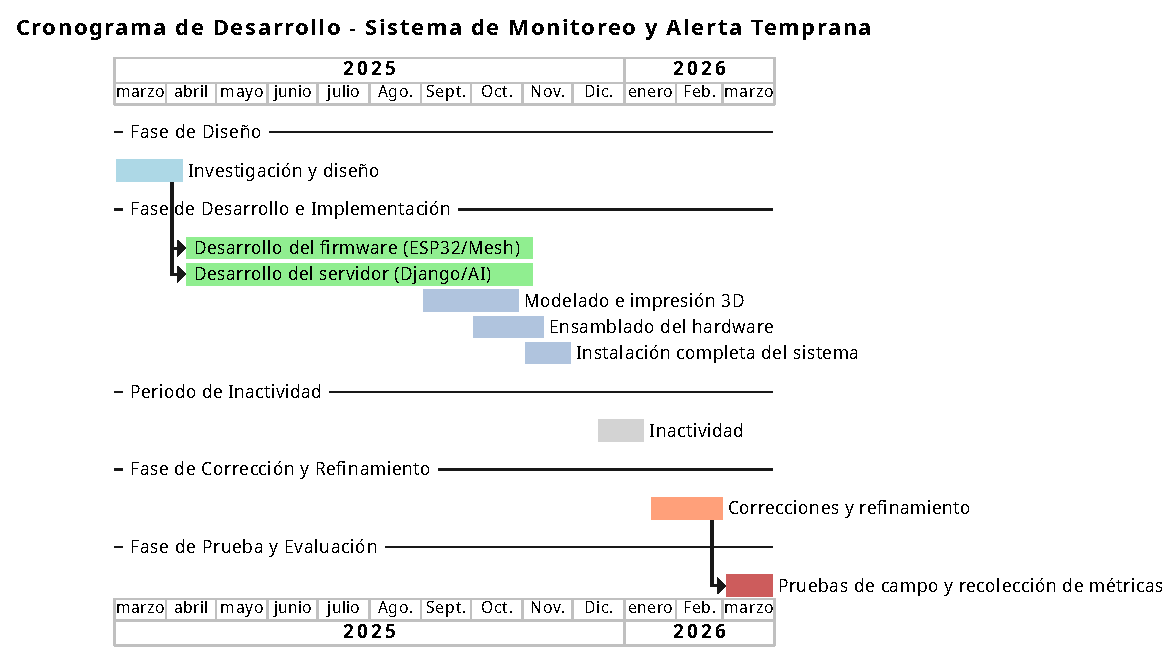
\includegraphics[width=\textwidth]{img/cronogramaDeDesarrollo.pdf}
  \caption{Cronograma de desarrollo del proyecto.}
  \label{fig:gantt-desarrollo}
\end{figure}

\section{Herramientas y tecnologías utilizadas}

\subsection{Entorno de desarrollo}

\begin{description}
  \item[Editor de código:] Visual Studio Code con extensiones para desarrollo
    en C/C++ (ESP-IDF), Python y Docker.
  \item[Framework de firmware:] \gls{ESP-IDF} con el componente
    \gls{ESP-MESH-LITE} para el desarrollo del código de los nodos
    \gls{ESP32}.
  \item[Framework web:] \gls{django} para el servidor de aplicación.
  \item[Bot de notificaciones:] Librería \texttt{python-telegram-bot} para
    la implementación del sistema de alertas mediante Telegram.
  \item[Contenedorización:] \gls{docker} y \gls{docker-compose} para el
    despliegue de servicios.
\end{description}

\subsection{Diseño y fabricación 3D}

\begin{description}
  \item[Software de modelado:] Autodesk Fusion 360 con licencia educativa para
    el diseño de la \gls{carcasa} del nodo.
  \item[Software de laminado:] PrusaSlicer para la preparación de modelos 3D
    y generación de \gls{gcode} para la impresora.
  \item[Impresora 3D:] Creality Ender 3 con cama caliente, utilizando filamento
    \gls{pla} para los prototipos de validación.
\end{description}

\subsection{Control de versiones y despliegue}

El código fuente del proyecto fue organizado en tres repositorios \gls{git} alojados
en GitHub:
\begin{enumerate}
  \item Repositorio del \gls{firmware} para las cámaras (nodo de cámara, nodo
    raíz y nodo repetidor):\\
    \url{https://github.com/GabyDs/trapcam_mesh}
  \item Repositorio del servidor de aplicación:\\
    \url{https://github.com/fabcontigiani/server-capstone-project}
  \item Repositorio del servidor de inferencia y anotación de imágenes:\\
    \url{https://github.com/fabcontigiani/wildlife-detection-capstone-project}
\end{enumerate}

% \subsection{Despliegue continuo}

% Se implementó una estrategia de \gls{despliegue-continuo} mediante \gls{github-actions}
% para automatizar las siguientes tareas:

% \begin{itemize}
%   \item Construcción automática de imágenes \gls{docker} al realizar cambios
%         en las ramas principales de los repositorios.
%   \item Publicación de las imágenes en el registro de contenedores de GitHub
%         (GitHub Container Registry).
% \end{itemize}

% Esta automatización garantizó que las versiones desplegadas del servidor
% siempre correspondieran al código más reciente validado, reduciendo errores
% humanos en el proceso de despliegue.

\section{Métricas de evaluación}

Para validar el cumplimiento de los objetivos del proyecto, se definieron las
siguientes métricas de evaluación:

\subsection{Métricas de rendimiento de red}

\begin{description}
  \item[Latencia de transmisión:] Tiempo transcurrido desde la captura de una
    imagen en el nodo hasta su recepción completa en el servidor. Se mide
    en segundos y representa la capacidad del sistema para proporcionar
    información en tiempos operativamente útiles.
  \item[Distancia máxima entre nodos:] Distancia física máxima a la cual dos
    nodos pueden mantener una conexión \gls{mesh} funcional, medida en
    metros. Esta métrica determina la densidad de nodos necesaria para
    cubrir un área determinada.
  \item[Estabilidad de la red:] Tasa de pérdida de paquetes y frecuencia de
    reconexiones durante operación prolongada. Una red estable debe
    mantener tasas de pérdida inferiores al \qty{5}{\percent}.
\end{description}

% \subsection{Métricas de clasificación}

% \begin{description}
%   \item[Precisión de detección:] Proporción de imágenes correctamente
%     clasificadas como conteniendo animales, personas, vehículos o
%     imágenes vacías.
%   \item[Precisión de clasificación taxonómica:] Para las imágenes con animales,
%     proporción de especies correctamente identificadas a nivel de familia
%     o género.
% \end{description}

\subsection{Métricas de consumo energético}

\begin{description}
  \item[Consumo promedio del nodo:] Consumo eléctrico promedio del nodo de
    cámara durante un ciclo típico de operación (espera + captura +
    transmisión), medido en miliamperios (\unit{mA}).
  \item[Autonomía estimada:] Tiempo de operación estimado con una batería de
    capacidad conocida, calculado a partir del consumo promedio.
\end{description}

\section{Estrategia de pruebas}

\subsection{Pruebas incrementales de firmware}

Durante el desarrollo del \gls{firmware}, cada módulo fue probado de forma
aislada antes de su integración:

\begin{itemize}
  \item Pruebas de captura de imagen con el módulo OV2640
  \item Pruebas de detección del sensor \gls{pir}
  \item Pruebas de conexión y transmisión \gls{mesh} entre nodos
  \item Pruebas de consumo energético
\end{itemize}

\subsection{Pruebas de integración}

Una vez validados los componentes individuales, se realizaron pruebas de
integración verificando:

\begin{itemize}
  \item Transmisión de imágenes desde nodos de cámara hasta el servidor
  \item Procesamiento de imágenes por el modelo de \gls{ia}
  \item Generación de notificaciones mediante el bot de \gls{telegram-bot}
\end{itemize}

\subsection{Pruebas de sistema}

Las pruebas del sistema completo se realizaron en dos fases:

\begin{description}
  \item[Fase 1 - Pruebas de laboratorio:] Validación del funcionamiento del
    sistema en condiciones controladas de interior, verificando la
    correcta integración de todos los componentes y midiendo las métricas
    de rendimiento base.
  \item[Fase 2 - Pruebas de campo:] Instalación del sistema en un entorno
    exterior bajo condiciones climáticas favorables. Durante varias horas
    se monitoreó el funcionamiento del sistema, registrando las métricas
    de latencia, estabilidad de red, consumo energético y precisión de
    clasificación en condiciones realistas.
\end{description}

% ==============================================================================
% Capítulo 7: Diseño e Implementación del Sistema
% ==============================================================================
\chapter{Diseño e Implementación del Sistema}

\section{Arquitectura general}

El sistema propuesto se divide conceptualmente en dos grandes bloques operativos que trabajan de forma coordinada para lograr la detección y notificación de eventos:

\begin{itemize}
  \item \textbf{Red MESH:} Constituye la infraestructura de despliegue en campo. Está compuesta por los nodos terminales (\textit{Leaf}), los nodos intermedios (\textit{Relay}) y el nodo puerta de enlace (\textit{Root}). Estos dispositivos conforman una red inalámbrica auto-gestionada mediante el protocolo \gls{ESP-MESH-LITE}, encargándose de la vigilancia del entorno, captura fotográfica y propagación de los datos hacia internet.
  \item \textbf{Backend:} Representa la infraestructura de procesamiento centralizado. Recibe de manera asíncrona las imágenes provenientes de la Red MESH, orquesta la inferencia mediante modelos de inteligencia artificial (\gls{speciesnet}), persiste los metadatos en una base de datos y emite alertas automáticas al usuario final a través de la integración con Telegram.
\end{itemize}

La Figura~\ref{fig:arquitectura-general} presenta un diagrama de alto nivel
de esta arquitectura.

\begin{figure}[h!]
  \centering
  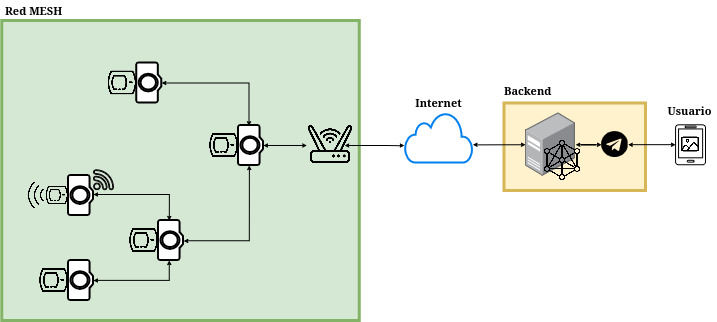
\includegraphics[width=.8\textwidth]{img/arquitecturaGeneralH.jpg}
  \caption{Arquitectura general del sistema de monitoreo, dividida en Red MESH y Backend.}
  \label{fig:arquitectura-general}
\end{figure}

\newpage

El flujo integral de la información opera de la siguiente manera:

\begin{enumerate}
  \item El sensor \gls{pir} de un nodo \textit{Leaf} o \textit{Relay} detecta movimiento, desencadenando la reactivación del microcontrolador desde su estado de reposo.
  \item El nodo captura una imagen en formato \gls{jpeg}.
  \item El nodo origina una petición HTTP POST dirigida al \textit{Backend}. Esta petición viaja saltando a través de los nodos \textit{Relay} de la red MESH hasta alcanzar al nodo \textit{Root}, quien finalmente la inyecta al router Wi-Fi para su salida a internet.
  \item El servidor recibe la imagen y delega su procesamiento al contenedor de \gls{speciesnet} (que ejecuta los modelos de detección y clasificación taxonómica).
  \item Si el análisis identifica objetos de interés superando el umbral de confianza predefinido, el bot de Telegram notifica al usuario de forma inmediata, adjuntando la evidencia visual (imágenes limpias y anotadas) y las probabilidades predictivas.
  \item Todos los eventos, clasificaciones e imágenes quedan respaldados en la base de datos relacional del sistema.
\end{enumerate}

\section{Nodos de cámara (Leaf y Relay)}

La arquitectura del sistema define dos roles distintos para los nodos equipados con cámara, a pesar de que ambos comparten el mismo hardware. Esta separación, definida mediante configuración, permite equilibrar el alcance de la red y el consumo energético:

\begin{itemize}
  \item \textbf{Nodo Intermedio (Relay):} Extiende la cobertura de la red permitiendo que otros nodos se conecten a él (actúa como router), además de realizar funciones de cámara. Utiliza modos de reposo ligero para mantener la conectividad MESH de forma constante.
  \item \textbf{Nodo Hoja (Leaf):} Nodo terminal enfocado en el ultra bajo consumo. Utiliza el modo de reposo profundo (\textit{Deep Sleep}) apagando su radio Wi-Fi y su CPU principal, despertando únicamente cuando el coprocesador detecta movimiento.
\end{itemize}

\subsection{Selección de componentes}

El nodo de cámara se construye alrededor de los siguientes componentes
principales:

\begin{description}
  \item[Microcontrolador:] Módulo ESP32-CAM de AI-Thinker, que integra un
    \gls{ESP32} con cámara OV2640 y ranura para tarjeta microSD en una
    placa compacta.
  \item[Sensor de movimiento:] Módulo HC-SR501, un sensor \gls{pir} de bajo
    costo con sensibilidad y tiempo de retardo ajustables mediante
    potenciómetros.
  \item[Regulador de voltaje:] Módulo \gls{buck-converter} basado en el
    circuito integrado LM2596, que acepta voltajes de entrada entre
    \qty{4.5}{V} y \qty{40}{V}, permitiendo alimentación desde packs de baterías
    \glspl{18650} en configuración 2S (\qty{7.4}{V} nominal).
\end{description}

\subsection{Diseño del firmware}

El firmware de los nodos de cámara se desarrolló utilizando \gls{ESP-IDF} y \gls{ESP-MESH-LITE}, adoptando un diseño modular. El arranque inicial y las configuraciones básicas son compartidas, mientras que la gestión de energía y el monitoreo de eventos difieren según el rol (Leaf o Relay).

El flujo general de ejecución (ilustrado en la Figura~\ref{fig:diagrama-flujo-general}) comprende:

\begin{itemize}
  \item Inicialización del sistema base (NVS, \textit{event loop}, interfaces de red).
  \item Configuración de la red \gls{ESP-MESH-LITE} en modo \gls{AP-STA} (o solo estación para los nodos hoja).
  \item Inicialización condicional de la tarjeta microSD.
  \item Configuración de las interrupciones o rutinas de detección correspondientes al sensor \gls{pir}.
  \item Una vez establecida la conexión MESH y obtenida una IP, se ejecuta la rutina de monitoreo. Si hay detección, se captura y envía la foto.
\end{itemize}

\begin{figure}[htbp]
  \centering
  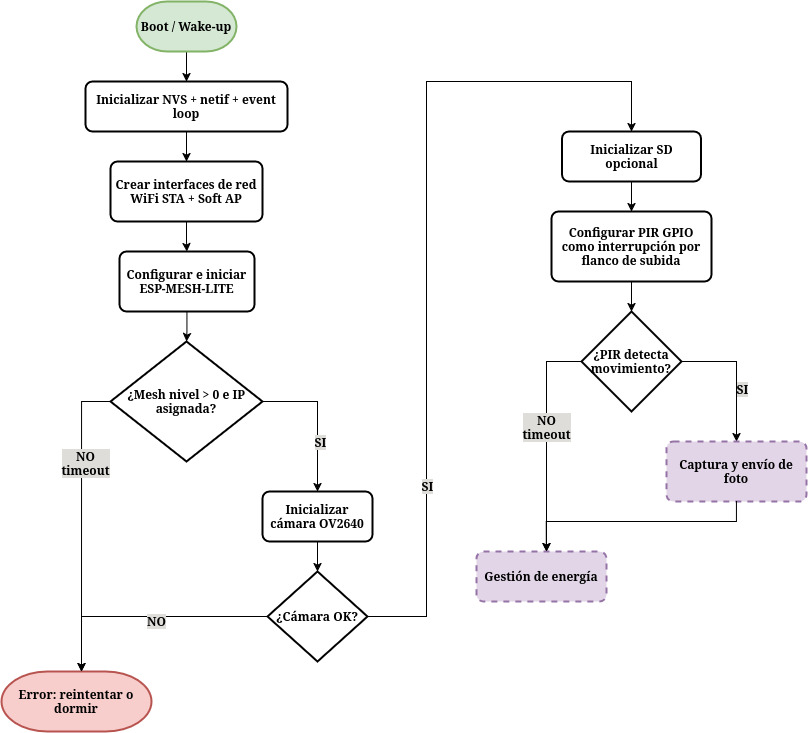
\includegraphics[width=0.6\textwidth]{img/Diagramas Tesis-Diagrama de Flujo General.jpg}
  \caption{Diagrama de flujo general de inicialización de los nodos de cámara.}
  \label{fig:diagrama-flujo-general}
\end{figure}

\newpage
Para el \textbf{Nodo Intermedio (Relay)}, el ciclo de vida (Figura~\ref{fig:diagrama-energia-relay}) aprovecha un modo de reposo ligero (\textit{Light Sleep}) gestionado de forma automática por el sistema operativo, permitiendo a la radio Wi-Fi utilizar \textit{Modem Sleep} pero manteniendo siempre la conectividad MESH activa. Una tarea de \gls{freertos} bloqueada espera una notificación del sensor PIR para proceder a la captura.

\begin{figure}[htbp]
  \centering
  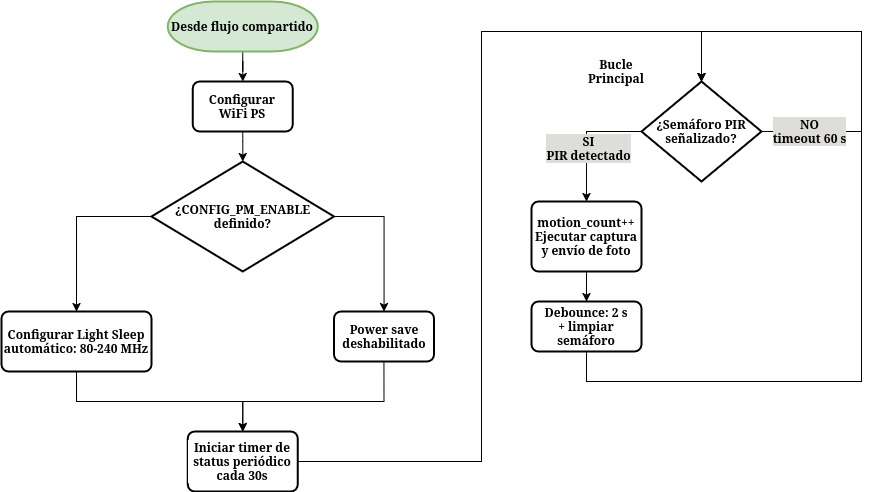
\includegraphics[width=0.75\textwidth]{img/Diagramas Tesis-Gestión de Energia nodo Raley Parte 1.jpg}

  \vspace{0.5cm}

  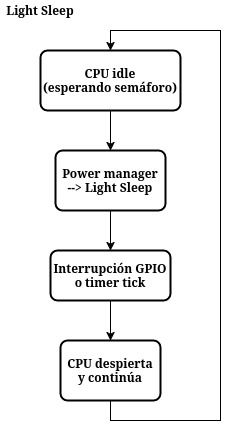
\includegraphics[width=0.3\textwidth]{img/Diagramas Tesis-Gestión de Energia nodo Raley Parte 2.jpg}
  \caption{Diagrama de gestión de energía del nodo intermedio (Relay).}
  \label{fig:diagrama-energia-relay}
\end{figure}

Para el \textbf{Nodo Hoja (Leaf)}, el flujo cambia drásticamente (Figura~\ref{fig:diagrama-energia-leaf}). Al no requerir mantener conexiones para otros nodos, el firmware apaga la interfaz Wi-Fi y pone al CPU principal en reposo profundo (\textit{Deep Sleep}). La vigilancia queda a cargo del coprocesador de ultra bajo consumo (\textbf{ULP}). Cuando se detecta movimiento, el coprocesador ULP despierta al CPU principal, el cual ejecuta el flujo compartido de reconexión, envía la foto, y vuelve a entrar en \textit{Deep Sleep}.

\begin{figure}[htbp]
  \centering
  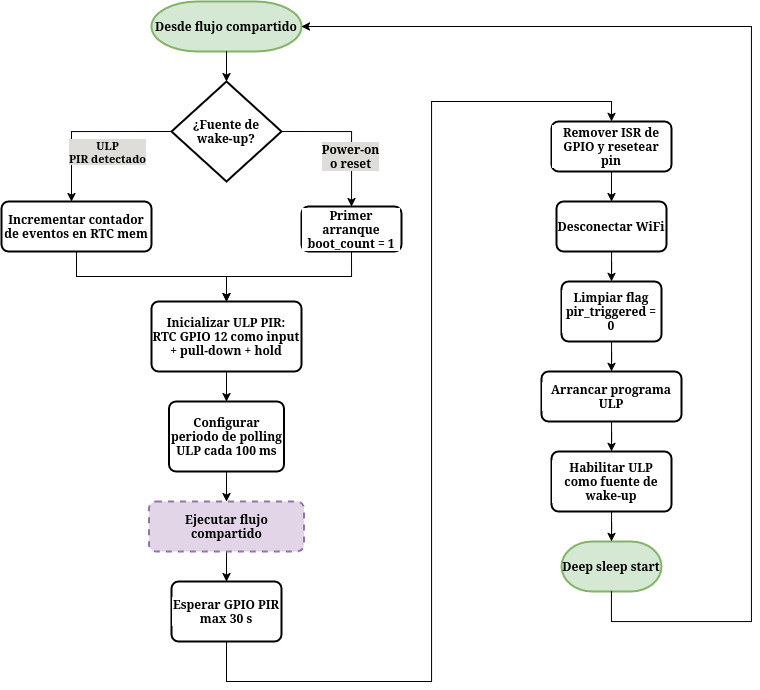
\includegraphics[width=0.7\textwidth]{img/Diagramas Tesis-Gestion de Energia nodo Leaf Parte 1.jpg}

  \vspace{0.3cm}

  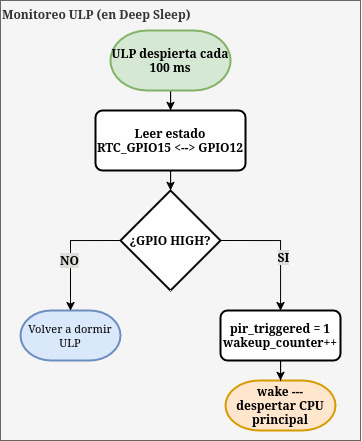
\includegraphics[width=0.3\textwidth]{img/Diagramas Tesis-Gestion de Energia nodo Leaf Parte 2.jpg}
  \caption{Diagrama de gestión de energía del nodo terminal (Leaf).}
  \label{fig:diagrama-energia-leaf}
\end{figure}

\newpage
\subsection{Captura y envío de imágenes}

La captura de imágenes se realiza con los siguientes parámetros:

\begin{description}
  \item[Resolución:] 640 $\times$ 480 píxeles (VGA)
  \item[Formato:] \gls{jpeg} con compresión configurable
  \item[Tamaño típico:] Entre 30 y 35 KB por imagen
\end{description}

El proceso detallado de la obtención del fotograma y su transmisión se describe en la Figura~\ref{fig:diagrama-captura}. La cámara requiere descartar los primeros fotogramas (\textit{warm-up}) para estabilizar los niveles de exposición y balance de blancos automáticos. Posteriormente, se evalúa la disponibilidad de la tarjeta SD para guardar una copia de respaldo antes de enviar el paquete HTTP POST mediante la red MESH.

\begin{figure}[htbp]
  \centering
  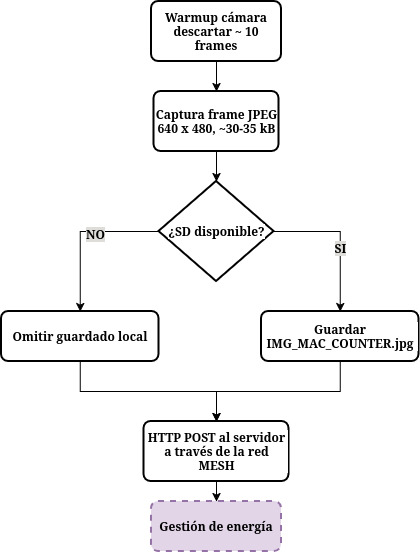
\includegraphics[width=0.6\textwidth]{img/Diagramas Tesis-Captura y Envio de Foto.jpg}
  \caption{Flujo de captura, almacenamiento y transmisión de imágenes.}
  \label{fig:diagrama-captura}
\end{figure}

Gracias a la arquitectura de \gls{ESP-MESH-LITE}, donde cada nodo posee su
propia pila de red \gls{lwip} y puede realizar peticiones HTTP de forma
independiente, no existen restricciones artificiales en el tamaño de los datos
transmitidos. El nivel de compresión se ajusta para balancear la calidad de
imagen con el tiempo de transmisión inalámbrica.

\subsection{Integración del sensor PIR}

El sensor HC-SR501 se conecta a un pin GPIO del ESP32-CAM. Dado que el sistema presenta dos modos de operación distintos, la integración del sensor se aborda mediante dos estrategias diferentes:

\begin{itemize}
  \item \textbf{En el nodo Relay:} El pin GPIO se configura como fuente de interrupción externa convencional. Al detectar movimiento, genera una señal HIGH que dispara una \gls{isr}. Esta rutina notifica a la tarea principal, despertando al CPU de su estado de \textit{Light Sleep} para procesar el evento.
  \item \textbf{En el nodo Leaf:} Durante el estado de \textit{Deep Sleep}, la matriz de interrupciones está apagada. La vigilancia se delega al coprocesador ULP. Como el ULP FSM no admite interrupciones de hardware, ejecuta un programa en ensamblador con un ciclo de \textit{polling} que despierta cada \qty{100}{ms} para leer el estado del registro RTC asociado al GPIO. Si detecta el estado HIGH, emite la instrucción \texttt{wake} para reactivar el CPU principal.
\end{itemize}

El sensor permite ajustar en su propio \textit{hardware}:
\begin{itemize}
  \item \textbf{Sensibilidad:} Distancia de detección (\qtyrange{3}{7}{m})
  \item \textbf{Tiempo de retardo:} Duración de la señal HIGH (\qtyrange{5}{300}{s})
\end{itemize}

El esquema de conexiones del nodo de cámara se incluye en el apéndice
\ref{fig:esquematico-mesh-node}.

\subsection{Transmisión}

La transmisión de imágenes aprovecha la arquitectura de capa de red IP de
\gls{ESP-MESH-LITE}. Cada nodo de cámara, al contar con su propia pila de
protocolos \gls{lwip} y una dirección IP asignada por su nodo padre, puede
realizar peticiones HTTP POST estándar hacia el servidor de aplicación.

Estas peticiones se propagan de forma transparente a través de los nodos
intermedios de la red mesh: cada nodo padre reenvía los paquetes en la capa
de red sin inspeccionar la capa de aplicación, hasta alcanzar el \gls{nodo-raiz}.
Este último, al ser el único nodo con conexión directa al router Wi-Fi, actúa
como puerta de enlace hacia la red externa, entregando los paquetes al servidor.

Desde la perspectiva del nodo de cámara, el proceso es equivalente a realizar
una petición HTTP convencional, lo que simplifica significativamente el
desarrollo del firmware al eliminar la necesidad de gestionar manualmente la
fragmentación, el reensamblado o el enrutamiento de datos.

\subsection{Carcasa para impresión 3D}

El diseño de la carcasa se basó en un modelo público bajo licencia
Creative Commons 4.0 International, disponible en
Printables\footnote{\url{www.printables.com/model/520378-case-for-esp32_cam-trail-camera-pir-sensor-18650-b}},
el cual fue modificado utilizando Autodesk Fusion 360 para adaptarlo a los
requerimientos específicos del proyecto. La carcasa fue impresa en \gls{pla}
y contempla:

\begin{itemize}
  \item Apertura frontal para la lente de la cámara
  \item Apertura superior para el domo del sensor PIR
  \item Espacio interno para el módulo \gls{buck-converter} basado en LM2596
  \item Orificio para cable de alimentación hacia pack de baterías externo
  \item Provisión para conexión de antena externa
  \item Ranura de acceso a la tarjeta microSD
  \item Puntos de montaje para fijación en superficies
\end{itemize}

El plano 2D del diseño final se incluye en el apéndice~\ref{anexo:planos-carcasa}
(Figura~\ref{fig:plano-carcasa} y Figura~\ref{fig:plano-base}). El modelo 3D
modificado está disponible públicamente en Printables\footnote{\url{www.printables.com/model/1532349-case-for-esp32_cam-trail-camera-pir-sensor-buck-co}}.
La figura~\ref{fig:modelo-3d-carcasa} muestra el modelo 3D de la carcasa.

\begin{figure}[htbp]
  \centering
  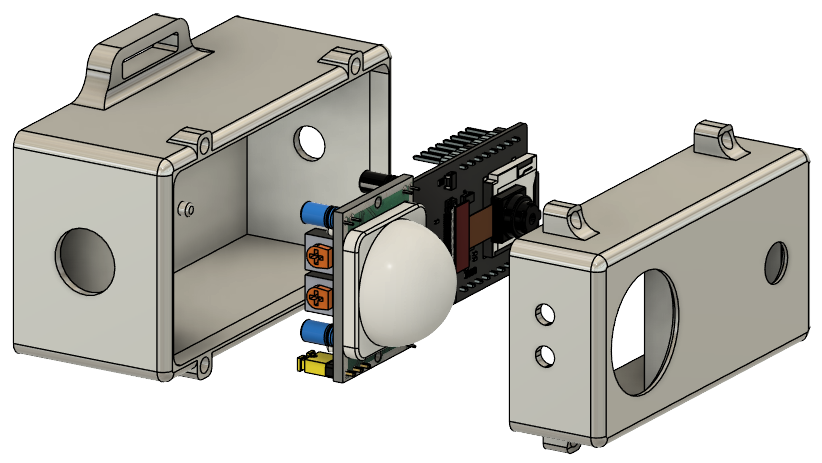
\includegraphics[width=0.8\textwidth]{img/modelo3D.png}
  % \fbox{\parbox{0.6\textwidth}{\centering\vspace{3cm}
  %     [Modelo 3D de la carcasa del nodo de cámara]
  %     \vspace{3cm}}}
  \caption{Modelo 3D de la carcasa del nodo de cámara.}
  \label{fig:modelo-3d-carcasa}
\end{figure}

\section{Nodo raíz (root-node)}

\subsection{Diseño del hardware}

El nodo raíz utiliza una placa de desarrollo ESP32 DevKit V1, sin
módulo de cámara, que actúa como puerta de enlace entre la red
\gls{mesh} y el servidor de aplicación.

\subsection{Firmware del nodo raíz}

El firmware del nodo raíz actúa como el coordinador central de la red mallada, garantizando la conectividad ininterrumpida de todo el sistema. A diferencia de los nodos de cámara, este componente opera exclusivamente como enrutador y servidor de la malla, excluyendo la carga de controladores periféricos (como la cámara OV2640 o el sensor PIR) y descartando el uso de modos de bajo consumo (\textit{Sleep Modes}).

La inicialización específica y el ciclo de vida del nodo raíz, ilustrados en la Figura~\ref{fig:diagrama-firmware-root}, implementan las siguientes responsabilidades clave:

\begin{itemize}
  \item \textbf{Jerarquía exclusiva:} Mediante la configuración del firmware, se fuerza al dispositivo a operar estrictamente en el Nivel 1 de la topología MESH, conectándose directamente al router Wi-Fi externo (modo \textit{Station}).
  \item \textbf{Punto de Acceso permanente:} La interfaz \textit{SoftAP} se mantiene siempre activa, aguardando y gestionando la conexión de nodos hijos (tanto intermedios como terminales).
  \item \textbf{Enrutamiento transparente:} Actuando como puente de red (\textit{Bridge}), provee NAT, asignación de direcciones IP dinámicas y reenvío de los paquetes provenientes de la malla hacia internet.
  \item \textbf{Gestión y diagnóstico:} Se registra un conjunto de manejadores de mensajes para interpretar la actividad de los nodos y se ejecuta un temporizador periódico que reporta el estado de la red (canal Wi-Fi, cantidad de hijos conectados, RSSI) cada 10 segundos.
  \item \textbf{Limpieza de rutas:} Se ajusta el \textit{timeout} de desconexión de la interfaz a 60 segundos para eliminar rápidamente de la tabla de ruteo a cualquier nodo hijo que haya perdido el enlace.
\end{itemize}

\begin{figure}[htbp]
  \centering
  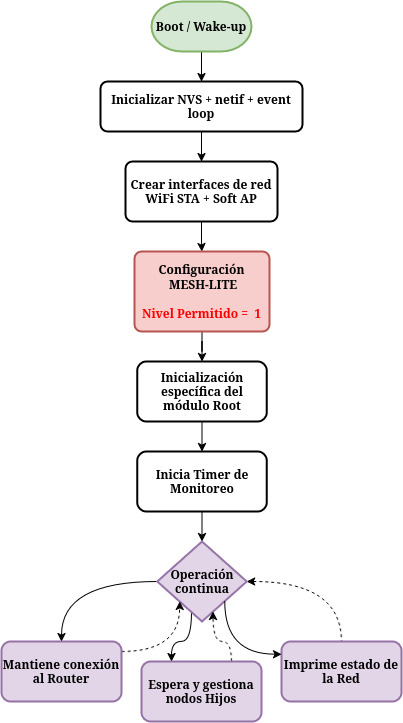
\includegraphics[width=0.7\textwidth]{img/Diagramas Tesis-Diagra de Flujo nodo Root.jpg}
  \caption{Diagrama de flujo de inicialización y operación continua del nodo raíz.}
  \label{fig:diagrama-firmware-root}
\end{figure}

\newpage
\subsection{Conexión con la red externa}

El nodo raíz es el único punto de salida a internet de la red mesh. Se conecta
a un router Wi-Fi doméstico como estación (STA), proporcionando a todos los
nodos de la red acceso a la red IP externa de forma transparente.

Cuando un nodo de cámara envía una petición HTTP al servidor, los paquetes
son reenviados nodo a nodo en la capa de red hasta alcanzar el nodo raíz,
que los entrega al router para su transmisión hacia el servidor. En la
sección de trabajos futuros se discute la posibilidad de reemplazar este
enlace por tecnologías de mayor alcance para despliegues en zonas remotas.

\subsection{Gestión de la red mesh}

El nodo raíz es responsable de:

\begin{itemize}
  \item Mantener la topología de la red mesh
  \item Gestionar la conexión y desconexión de nodos hijos
  \item Actuar como puerta de enlace IP para toda la red
  \item Proporcionar sincronización de tiempo a la red
\end{itemize}

La red está configurada para soportar hasta 6 niveles de profundidad,
aunque en las pruebas realizadas se utilizaron únicamente 3 nodos.

\section{Red mesh}

\subsection{Topología de la red}

La red \gls{ESP-MESH-LITE} se organiza en una topología de árbol, donde cada nodo asume uno de los siguientes roles configurables:

\begin{description}
  \item[Nodo raíz (Root):] Nivel 1. Único punto de conexión con la red externa (router Wi-Fi). Actúa como puerta de enlace IP para toda la red mesh y permanece activo ininterrumpidamente.
  \item[Nodos intermedios (Relay):] Extienden la red actuando como padres para otros nodos y reenviando paquetes de forma transparente en la capa de red. Simultáneamente, funcionan como cámaras utilizando modos de reposo ligero para no interrumpir el enrutamiento.
  \item[Nodos hoja (Leaf):] Nodos de cámara terminales que no permiten la conexión de hijos. Se dedican exclusivamente a la captura y operan mayormente en reposo profundo (\textit{Deep Sleep}) para maximizar la autonomía.
\end{description}

Cada nodo opera en modo \gls{AP-STA}, actuando simultáneamente como
punto de acceso para nodos hijos y como estación conectada a su nodo padre.
Cada nodo habilita su propia pila de protocolos \gls{lwip}, obteniendo una
dirección IP que le permite comunicarse de forma independiente con la red
externa.

% La Figura~\ref{fig:topologia-mesh} ilustra la topología de la red y el flujo
% de datos desde los nodos de cámara hasta el servidor.

% \begin{figure}[htbp]
%   \centering
%   % \includegraphics[width=0.8\textwidth]{figures/topologia-mesh.png}
%   \fbox{\parbox{0.8\textwidth}{\centering\vspace{3cm}
%       [Topología de la red ESP-MESH-LITE y flujo de datos]
%   \vspace{3cm}}}
%   \caption{Topología de la red ESP-MESH-LITE y flujo de datos.}
%   \label{fig:topologia-mesh}
% \end{figure}

\subsection{Protocolo de comunicación}

La comunicación utiliza el protocolo \gls{ESP-MESH-LITE} implementado sobre
Wi-Fi 802.11, con las siguientes características:

\begin{itemize}
  \item Autoorganización: los nodos seleccionan su padre óptimo basándose
    en \gls{rssi}
  \item \Gls{autocuracion}: reconexión automática ante fallos de nodos
  \item Reenvío transparente en capa de red: los nodos intermedios propagan
    paquetes sin inspeccionar la capa de aplicación
  \item Acceso independiente a red: cada nodo puede realizar peticiones HTTP
    de forma autónoma
\end{itemize}

\subsection{Formato de datos}

Las imágenes se transmiten mediante peticiones HTTP POST estándar desde cada
nodo de cámara hacia el servidor de aplicación. Cada petición incluye la imagen
en formato \gls{jpeg} como cuerpo de la solicitud, junto con metadatos
(identificador del nodo origen, timestamp) en los encabezados HTTP.

\section{Servicio de detección (wildlife-detection)}

\subsection{Arquitectura del servicio}

El servicio de detección se implementa como un contenedor \gls{docker}
independiente que expone una \gls{api} REST para la inferencia de imágenes.

\subsection{Contenedor Docker con SpeciesNet}

El contenedor incluye:

\begin{itemize}
  \item \gls{megadetector} (basado en la arquitectura \gls{yolov5}) para la detección y localización de animales, personas y vehículos.
  \item Modelos clasificadores taxonómicos de \gls{speciesnet} para predecir la especie de los animales detectados.
  \item Servidor HTTP basado en LitServe para manejar las peticiones concurrentes.
\end{itemize}

\subsection{API de inferencia}

El servicio expone un gls{endpoint} \texttt{/predict} que:

\begin{enumerate}
  \item Recibe una solicitud con la ruta local de una imagen en formato \gls{jpeg}.
  \item Ejecuta el pipeline interno de detección, clasificación y dibujado.
  \item Retorna las detecciones con sus respectivas \glspl{bounding-box}, niveles de confianza, etiquetas taxonómicas y la ruta de la imagen procesada con las anotaciones visuales.
\end{enumerate}

\subsection{Detección y clasificación}

Como ilustra la Figura~\ref{fig:pipeline-speciesnet}, el pipeline de procesamiento de imágenes dentro del contenedor opera en tres fases principales:

\begin{enumerate}
  \item \textbf{Detección:} \gls{megadetector} identifica regiones de interés en la imagen original, clasificándolas a alto nivel como animal, persona o vehículo, y genera las cajas delimitadoras.
  \item \textbf{Clasificación:} Para los recortes de las regiones detectadas específicamente como animales, se aplican los modelos de \gls{speciesnet} que analizan la imagen y predicen su familia, género y especie.
  \item \textbf{Anotación visual:} Se utilizan las \glspl{bounding-box} de la etapa de detección junto con las etiquetas de la etapa de clasificación para generar y guardar una nueva copia de la imagen con los resultados dibujados.
\end{enumerate}

\begin{figure}[htbp]
  \centering
  \begin{tikzpicture}[
      node distance=1.2cm and 2cm,
      box/.style={rectangle, draw, rounded corners, fill=blue!10, text width=4cm, text centered, minimum height=1.5cm, font=\sffamily\small},
      io/.style={trapezium, trapezium left angle=70, trapezium right angle=110, draw, fill=green!10, text width=3.5cm, text centered, minimum height=1.2cm, font=\sffamily\small},
      process/.style={rectangle, draw, fill=orange!10, text width=4cm, text centered, minimum height=1.5cm, font=\sffamily\small},
      arrow/.style={thick, -Latex}
    ]

    % Nodos
    \node (request) [io] {HTTP POST \texttt{/predict}\\ (Ruta de imagen)};
    \node (read) [process, below=of request] {Lectura de Imagen\\ (Volumen Docker)};
    \node (detect) [box, below=of read] {Modelo de Detección\\ (MegaDetector)\\ \textit{Localiza animales, personas, vehículos}};
    \node (classify) [box, below=of detect] {Modelo Clasificación\\ (SpeciesNet)\\ \textit{Identifica especies}};
    \node (draw) [process, below=of classify] {Generación de Imagen\\ Anotada};
    \node (save) [process, below=of draw] {Guardado de Imagen\\ (Volumen Docker)};
    \node (response) [io, below=of save] {Respuesta JSON\\ (Detecciones, Especies)};

    % Contenedor agrupado
    \begin{scope}[on background layer]
      \node[fill=blue!5, rounded corners, draw=blue!50, dashed, inner sep=15pt, fit=(read) (detect) (classify) (draw) (save), label={[font=\sffamily\bfseries, blue!80!black]above left:Contenedor Docker SpeciesNet}] (container) {};
    \end{scope}

    % Conexiones
    \draw [arrow] (request) -- (read);
    \draw [arrow] (read) -- (detect);
    \draw [arrow] (detect) -- node[anchor=east, align=center, font=\scriptsize] {Recortes} (classify);
    \draw [arrow] (classify) -- node[anchor=east, align=center, font=\scriptsize] {Clases y\\Confianza} (draw);
    \draw [arrow] (draw) -- (save);
    \draw [arrow] (save) -- (response);

    % Bounding boxes directos al dibujado
    \draw [arrow] (detect.east) -- ++(1.5,0) |- node[pos=0.25, anchor=west, align=center, font=\scriptsize] {Bounding\\Boxes} (draw.east);

  \end{tikzpicture}
  \caption{Pipeline de detección y clasificación interno del contenedor SpeciesNet.}
  \label{fig:pipeline-speciesnet}
\end{figure}

\section{Servidor de aplicación (server)}

El servidor de aplicación actúa como el núcleo central del sistema, coordinando la recepción de imágenes, el procesamiento de las mismas mediante algoritmos de inteligencia artificial y la emisión de alertas. Este componente fue desarrollado utilizando el \textit{framework} web \gls{django} (versión 5.2) sobre el lenguaje Python (versión 3.13), estructurando así la lógica principal del \textit{software}.

\subsection{Arquitectura del procesamiento}

La arquitectura del servidor implementa los siguientes componentes clave:

\begin{itemize}
  \item \textbf{\Gls{endpoint} HTTP:} para la recepción asíncrona de imágenes provenientes de los nodos de cámara dentro de la red mesh.
  \item \textbf{Integración IA:} comunicación vía HTTP REST con el servicio local de inferencia de \gls{speciesnet}.
  \item \textbf{Persistencia:} almacenamiento estructurado de imágenes y metadatos en una base de datos \gls{postgresql} (versión 15).
  \item \textbf{Sistema de notificaciones:} integración con un bot de Telegram, implementado mediante la librería \texttt{python-telegram-bot}, para la emisión automatizada de alertas.
  \item \textbf{Interfaz web de monitoreo:} panel para la visualización en tiempo real de las últimas imágenes recibidas y procesadas.
\end{itemize}

El flujo de procesamiento en el servidor opera de la siguiente manera:

\begin{enumerate}
  \item El \gls{endpoint} HTTP recibe una imagen enviada por un nodo de cámara a través de la red de comunicaciones.
  \item La imagen recibida se almacena en el sistema de archivos del servidor. De manera simultánea, se registra su entrada en la base de datos junto con los metadatos asociados (tales como el identificador del nodo de origen y el \textit{timestamp} de captura).
  \item Inmediatamente después del registro, la imagen se envía al servicio de inferencia de IA (\gls{speciesnet}) mediante una petición HTTP interna.
  \item El servicio de inferencia analiza la imagen mediante su modelo subyacente (basado en YOLOv5) y retorna las detecciones encontradas (categorías detectadas como animales, humanos o vehículos, junto con sus valores de confianza y coordenadas de las \glspl{bounding-box}), así como las clasificaciones taxonómicas de las especies.
  \item Los resultados de la inferencia se almacenan de manera relacional en la base de datos. Además, se recupera y guarda una copia procesada de la imagen que incluye las anotaciones gráficas de las \glspl{bounding-box}.
  \item El sistema evalúa los resultados mediante un filtro de lógica de negocio. Si alguna de las detecciones supera el umbral de confianza previamente configurado y representa un objeto de interés, el bot de Telegram se encarga de enviar una notificación al usuario. Esta alerta incluye la imagen original, la imagen procesada y un resumen detallado de las detecciones y clasificaciones.
\end{enumerate}

La Figura~\ref{fig:diagrama-flujo-servidor} ilustra gráficamente este flujo de procesamiento integral.

\begin{figure}[htbp]
  \centering
  \begin{tikzpicture}[
      node distance=1.2cm and 2cm,
      box/.style={rectangle, draw, rounded corners, fill=blue!10, text width=4cm, text centered, minimum height=1.5cm, font=\sffamily\small},
      io/.style={trapezium, trapezium left angle=70, trapezium right angle=110, draw, fill=green!10, text width=3.5cm, text centered, minimum height=1.2cm, font=\sffamily\small},
      process/.style={rectangle, draw, fill=orange!10, text width=4cm, text centered, minimum height=1.5cm, font=\sffamily\small},
      decision/.style={diamond, draw, fill=red!10, text width=2.5cm, text badly centered, inner sep=0pt, font=\sffamily\small},
      arrow/.style={thick, -Latex}
    ]
    \node [io] (receive) {Recepción de imagen (HTTP)};
    \node [process, below=of receive] (store) {Almacenar en FS y registrar metadatos en BD};
    \node [process, below=of store] (infer) {Inferencia \gls{speciesnet} (Detección y Clasificación)};
    \node [process, below=of infer] (process_res) {Guardar resultados (BD) y procesar imagen anotada};
    \node [decision, below=of process_res, yshift=-0.3cm] (threshold) {¿Supera umbral?};
    \node [box, right=of threshold, xshift=1cm] (telegram) {Alerta vía Telegram bot};
    \node [box, below=of threshold, yshift=-0.3cm] (end) {Fin del procesamiento};

    \draw [arrow] (receive) -- (store);
    \draw [arrow] (store) -- (infer);
    \draw [arrow] (infer) -- (process_res);
    \draw [arrow] (process_res) -- (threshold);
    \draw [arrow] (threshold) -- node[anchor=south] {Sí} (telegram);
    \draw [arrow] (threshold) -- node[anchor=east] {No} (end);
    \draw [arrow] (telegram) |- (end);
  \end{tikzpicture}
  \caption{Diagrama de flujo del procesamiento de imágenes en el servidor.}
  \label{fig:diagrama-flujo-servidor}
\end{figure}

La interfaz web proporciona, a su vez, una vista de monitoreo que muestra las últimas imágenes recibidas junto con sus resultados de detección. Esta interfaz fue desarrollada como una herramienta auxiliar de desarrollo y depuración para visualizar las capacidades predictivas del modelo, y no forma parte de la vista principal que reciben los usuarios a través del sistema de alertas en Telegram.

\subsection{Gestión de imágenes}

Las imágenes se administran y almacenan en un volumen compartido configurado en \gls{docker}, facilitando el acceso simultáneo desde distintos servicios. Se conservan dos variantes principales:

\begin{itemize}
  \item \textbf{Imágenes originales:} los archivos puros tal como son recibidos desde los nodos de cámara periféricos.
  \item \textbf{Imágenes anotadas:} archivos procesados que incluyen gráficamente las \glspl{bounding-box} generadas por el servicio de detección, permitiendo una rápida verificación visual.
\end{itemize}

Para optimizar el uso de los recursos del motor relacional, en la base de datos se almacenan únicamente las rutas relativas (paths) a los archivos físicos de las imágenes, enlazadas con la totalidad de los metadatos de las detecciones, confianzas y clasificaciones.

\subsection{Bot de Telegram y sistema de alertas}

El componente de interacción con el usuario final se materializa a través de un bot en la plataforma Telegram, desarrollado mediante la librería \texttt{python-telegram-bot}. Dada la naturaleza de los datos y los tiempos de procesamiento de los modelos de inteligencia artificial, la arquitectura del bot se diseñó bajo un paradigma asíncrono, garantizando la no interrupción de los procesos concurrentes del servidor principal.

La interacción con el usuario se estructura en tres capacidades funcionales:

\subsubsection{Suscripción y gestión de usuarios}

Para que el servidor pueda emitir notificaciones focalizadas, se requiere un proceso previo de emparejamiento. Mediante el comando de inicialización \texttt{/start}, el bot registra al usuario en la base de datos relacional, almacenando su identificador de chat (\textit{chat ID}) y sus datos de perfil. Este registro permite al sistema identificar inequívocamente a los destinatarios autorizados para recibir las alertas automáticas de seguridad.

\subsubsection{Emisión automatizada de alertas proactivas}

El núcleo del sistema de notificaciones radica en su capacidad de alerta autónoma. Al finalizar la etapa de inferencia de cada captura, un filtro lógico evalúa los resultados arrojados por el modelo. Si los objetos clasificados superan el umbral de confianza prestablecido, el bot compone y transmite de manera inmediata una alerta a los usuarios suscritos.

Cada notificación consolida la evidencia empírica en un único paquete (\textit{Media Group}), estructurado de la siguiente manera:

\begin{itemize}
  \item La fotografía original en alta definición capturada por el nodo sensor de la red.
  \item Una copia gráfica de la imagen que incluye trazadas las \glspl{bounding-box} de cada una de las detecciones generadas por \gls{speciesnet}.
  \item Un desglose textual que detalla la cantidad de objetos detectados y sus métricas probabilísticas de confianza.
  \item Las cinco principales etiquetas de clasificación taxonómica (\textit{top 5}) asociadas a la predicción, organizadas en orden decreciente de certeza.
\end{itemize}

\subsubsection{Consultas interactivas bajo demanda}

De manera complementaria al flujo de alertas automáticas, el sistema proporciona comandos de interacción manual. Mediante el uso del comando \texttt{/last}, el bot realiza una consulta a la base de datos para recuperar la fotografía más reciente ingresada al servidor, independientemente de si las clasificaciones superaron o no el filtro de notificaciones. Esta funcionalidad facilita a los operadores la realización de auditorías y la monitorización operativa de la red en tiempo real.

\subsubsection{Retroalimentación interactiva y corrección manual (\textit{Human-in-the-loop})}

Para refinar la precisión del sistema y mitigar posibles falsos positivos, el bot incorpora un mecanismo de retroalimentación interactiva directamente en los mensajes de alerta. A través de teclados integrados (\textit{inline keyboards}), los operadores pueden confirmar o rechazar la clasificación taxonómica inicial provista por el modelo de IA.

En caso de identificar una clasificación incorrecta, el sistema despliega dinámicamente un menú de selección múltiple presentando las especies alternativas sugeridas por la inferencia. Al confirmar la corrección, el bot actualiza el registro correspondiente en la base de datos, persistiendo la nueva etiqueta taxonómica y marcando el evento como auditado manualmente.

Esta integración del usuario en el ciclo de vida del procesamiento (\textit{Human-in-the-loop}) trasciende la simple corrección de errores en tiempo real y dota al sistema de una ventaja estratégica fundamental: la generación orgánica de un conjunto de datos altamente curado y etiquetado con precisión (\textit{Ground Truth}). Al acumular un volumen significativo de imágenes validadas correspondientes a la fauna endémica local —capturadas bajo las condiciones lumínicas reales y los ángulos específicos de las cámaras instaladas en terreno— se abre la posibilidad directa de aplicar técnicas de \textit{fine-tuning} (ajuste fino) o \textit{transfer learning} (transferencia de aprendizaje). De este modo, los modelos preentrenados genéricos pueden ser reentrenados y especializados iterativamente, logrando un sistema de inteligencia artificial que evoluciona y mejora de manera continua su capacidad de detección para el ecosistema particular de despliegue.

\subsection{Base de datos PostgreSQL}

La persistencia de los datos se fundamenta en el sistema gestor de bases de datos relacionales \gls{postgresql} (versión 15), estructurado para almacenar los distintos registros operativos del servidor:

\begin{itemize}
  \item \textbf{Registros fotográficos:} vínculos a los archivos físicos en el sistema de archivos junto a timestamps exactos.
  \item \textbf{Resultados de IA:} extracción del JSON de respuesta de la API, incluyendo clases detectadas, porcentajes de confianza y coordenadas de las \glspl{bounding-box}.
  \item \textbf{Taxonomía:} resultados detallados de la predicción de especies.
  \item \textbf{Auditoría y retroalimentación:} registro de las validaciones y correcciones manuales aportadas por los operadores a través del mecanismo \textit{Human-in-the-loop}, almacenando el estado de auditoría de cada evento y la etiqueta taxonómica definitiva.
  \item \textbf{Usuarios de Telegram:} registro de los IDs de los \textit{chats} que deben recibir las notificaciones push.
\end{itemize}

\subsection{Despliegue con Docker Compose}

Con el propósito de estandarizar el entorno de ejecución y asegurar su reproducibilidad, el servidor y sus dependencias se despliegan utilizando la herramienta de orquestación de contenedores \gls{docker-compose}. Esta configuración define e interconecta los siguientes servicios:

\begin{itemize}
  \item \textbf{Contenedor \gls{django}:} que ejecuta de forma concurrente el servidor web (utilizando Gunicorn y trabajadores Uvicorn) para atender el \gls{endpoint} HTTP, así como un proceso secundario o \textit{polling} para la ejecución del bot de Telegram.
  \item \textbf{Contenedor \gls{postgresql}:} servicio de base de datos aprovisionado de forma automatizada mediante variables de entorno y persistido con volúmenes locales.
  \item \textbf{Contenedor \gls{speciesnet}:} un servicio pre-compilado e instanciado localmente que encapsula el modelo de inferencia de IA. Esto elimina la dependencia de servicios externos de Google, mejorando la latencia del sistema y los requisitos de conectividad.
\end{itemize}

Los contenedores se comunican a través de una red interna aislada, administrada por la plataforma Docker. El contenedor principal, correspondiente a la aplicación Django, expone los puertos necesarios hacia el exterior para permitir la recepción de fotografías desde la red mesh. A su vez, establece conexiones privadas e internas tanto con el servicio de base de datos como con la API RESTful de inferencia, alojada en su contenedor respectivo. La Figura~\ref{fig:docker-compose-arquitectura} presenta de manera esquemática la disposición de los contenedores y sus flujos de datos.

\begin{figure}[htbp]
  \centering
  \begin{tikzpicture}[
      scale=0.8,
      font=\sffamily,
      >=Latex,
      node distance=14mm and 22mm,
      service/.style={
        draw=black!70,
        rounded corners=2pt,
        fill=blue!3,
        minimum width=22mm,
        minimum height=9mm,
        align=center,
        line width=0.9pt
      },
      volume/.style={
        draw=black!70,
        cylinder,
        shape border rotate=90,
        aspect=0.28,
        minimum height=9mm,
        minimum width=18mm,
        align=center,
        fill={rgb,255:red,253;green,250;blue,228},
        draw={rgb,255:red,134;green,122;blue,34},
        line width=0.9pt
      },
      bindmount/.style={
        draw=black!70,
        diamond,
        aspect=2,
        inner xsep=2pt,
        inner ysep=1.5pt,
        fill={rgb,255:red,253;green,250;blue,228},
        draw={rgb,255:red,134;green,122;blue,34},
        line width=0.9pt,
        font=\ttfamily\footnotesize,
        align=center
      },
      app/.style={-{Latex[length=2.2mm,width=1.6mm]}, draw=black!70, line width=0.95pt},
      mount/.style={Latex-Latex, draw=black!65, dashed, line width=0.95pt}
    ]

    % Service nodes
    \node[service] (web) {web};
    \node[service, left=of web] (bot) {bot};
    \node[service, right=of web] (db) {db};
    \node[service, below=of web] (speciesnet) {speciesnet};

    % Volume and bind mount nodes
    \node[bindmount, above left=18mm and 18mm of web] (Vstatic) {./static};
    \node[bindmount, above=of web] (Vmonitorstatic) {./monitor/static};
    \node[volume, left=34mm of speciesnet] (Vmediavolume) {media\_volume};
    \node[volume, below=of speciesnet] (Vspeciesnetcache) {speciesnet\_cache};
    \node[volume, below=of db] (Vdbdata) {db\_data};

    % Inter-service communication
    \draw[app] (bot) -- (web);
    \draw[app] (web) -- (db);
    \draw[app] (web) -- (speciesnet);

    % Volume mounts / bind mounts
    \draw[mount] (Vstatic) -- node[above, sloped, fill=white, inner sep=1pt, font=\ttfamily\scriptsize] {/app/static} (web);
    \draw[mount] (Vmonitorstatic) -- node[right, fill=white, inner sep=1pt, font=\ttfamily\scriptsize] {/app/monitor/static} (web);
    \draw[mount] (Vmediavolume) -- node[above, sloped, fill=white, inner sep=1pt, font=\ttfamily\scriptsize] {/app/media} (web);
    \draw[mount] (Vmediavolume) -- node[below, sloped, fill=white, inner sep=1pt, font=\ttfamily\scriptsize] {/app/media} (bot);
    \draw[mount] (Vspeciesnetcache) -- node[right, fill=white, inner sep=1pt, font=\ttfamily\scriptsize] {/app/.cache} (speciesnet);
    \draw[mount] (Vmediavolume) -- node[below, sloped, fill=white, inner sep=1pt, font=\ttfamily\scriptsize] {/app/media} (speciesnet);
    \draw[mount] (Vdbdata) -- node[right, fill=white, inner sep=1pt, font=\ttfamily\scriptsize] {/var/lib/postgresql/data} (db);

  \end{tikzpicture}
  \caption{Arquitectura de contenedores Docker del servidor.}
  \label{fig:docker-compose-arquitectura}
\end{figure}

\section{Alimentación y consumo energético}

Los nodos de cámara se alimentan mediante packs de \glspl{18650}
en configuración 2S (dos celdas en serie), proporcionando un voltaje
nominal de \qty{7.4}{V}. El módulo \gls{buck-converter} LM2596 reduce este
voltaje a \qty{5}{V} para alimentar el ESP32-CAM.

Para maximizar la autonomía sin comprometer la conectividad de la red, el sistema implementa una arquitectura híbrida de gestión de energía, donde el consumo varía drásticamente según el rol y el estado de operación:

\begin{description}
  \item[Modo Híbrido - Relay (\textit{Light Sleep + Modem Sleep}):] Los nodos intermedios deben mantener su conexión a la red \gls{ESP-MESH-LITE} para no romper la topología y permitir el enrutamiento. Utilizan un modo de ahorro donde la radio Wi-Fi se apaga parcialmente entre balizas y el CPU entra en \textit{Light Sleep}. Este estado reduce el consumo, pero requiere que el nodo esté parcialmente activo.
  \item[Modo Híbrido - Leaf (\textit{Deep Sleep + ULP}):] Los nodos terminales, al no enrutar tráfico de terceros, entran en un estado de \textit{Deep Sleep} desconectándose completamente de la red. El consumo se reduce drásticamente (alrededor de \qty{10}{mA} a \qty{15}{mA} reales medidos en el prototipo, atribuibles mayormente al módulo regulador y la placa), ya que el trabajo de monitoreo queda exclusivamente a cargo del coprocesador ULP.
  \item[Captura de imagen:] Consumo elevado momentáneo durante la activación
    del sensor OV2640, la captura de la imagen y la compresión \gls{jpeg}
    en hardware.
  \item[Transmisión:] Máximo consumo (alcanzando casi \qty{200}{mA}) durante la reconexión y el envío de la petición HTTP POST a través de la red mesh, con la radio Wi-Fi operando a máxima potencia.
\end{description}

Esta dualidad en la arquitectura de energía permite combinar las fortalezas de la red \gls{ESP-MESH-LITE} con técnicas avanzadas de ahorro energético, resolviendo la restricción típica de las redes malladas donde el requerimiento de enrutamiento continuo penaliza la vida útil de las baterías en nodos puramente sensoriales. (Las mediciones detalladas de corriente y autonomía se presentan en el Capítulo 8).

% ==============================================================================
% Capítulo 8: Pruebas y Resultados
% ==============================================================================
\chapter{Pruebas y Resultados}

\section{Ambiente de pruebas}

Para evaluar el desempeño operativo del sistema, se definió un entorno de pruebas diseñado para replicar las condiciones de un despliegue real. El mismo detalla puntualmente la configuración de hardware distribuido y la infraestructura de servidor empleadas.

\subsection{Infraestructura de hardware}

Las pruebas se ejecutaron sobre una red compuesta por tres nodos de cámara, ensamblados a partir de módulos ESP32-CAM acoplados a sensores infrarrojos pasivos (PIR) modelo HC-SR501. La coordinación del tráfico inalámbrico recayó sobre un nodo raíz implementado con una placa ESP32 DevKit V1, conectado a un enrutador Wi-Fi doméstico para proporcionar acceso externo.

Los dispositivos se energizaron utilizando paquetes de baterías \glspl{18650} en configuración 2S. Adicionalmente, el procesamiento se llevó a cabo en un servidor local provisto de un procesador multinúcleo, realizando las tareas de inferencia exclusivamente en la CPU, prescindiendo de aceleración gráfica dedicada (GPU).

\begin{figure}[htbp]
  \centering
  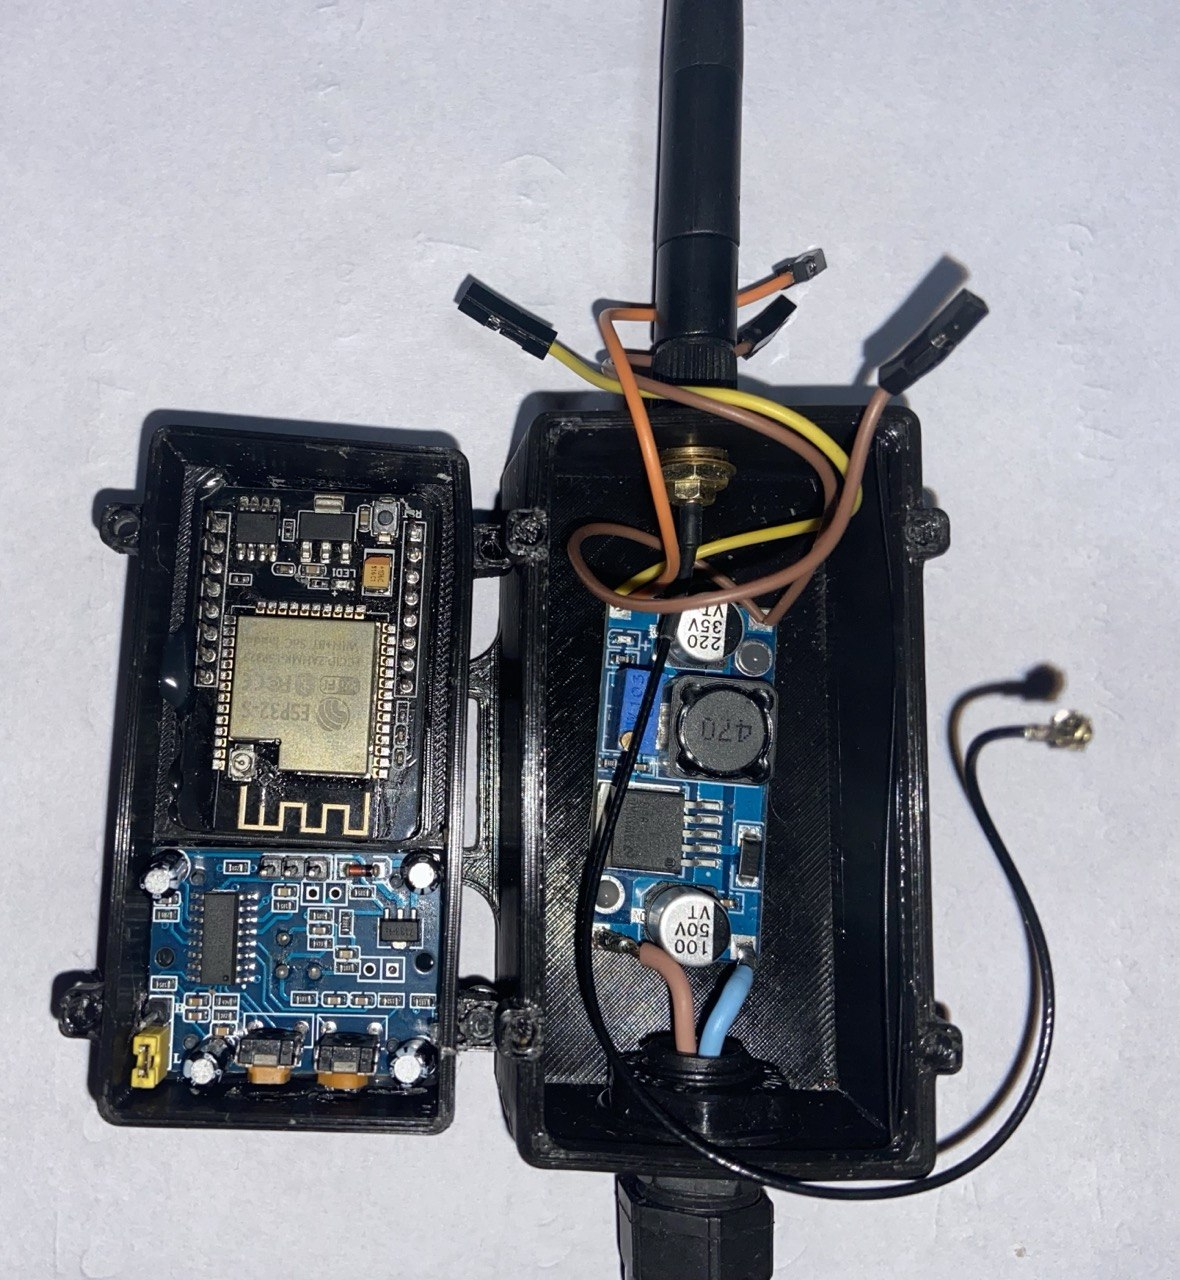
\includegraphics[width=0.5\textwidth]{img/carcasa_componentes_ensamblados.jpg}
  \caption{Carcasa impresa en PLA con componentes instalados.}
  \label{fig:carcasa-impresa}
\end{figure}

\begin{figure}[htbp]
  \centering
  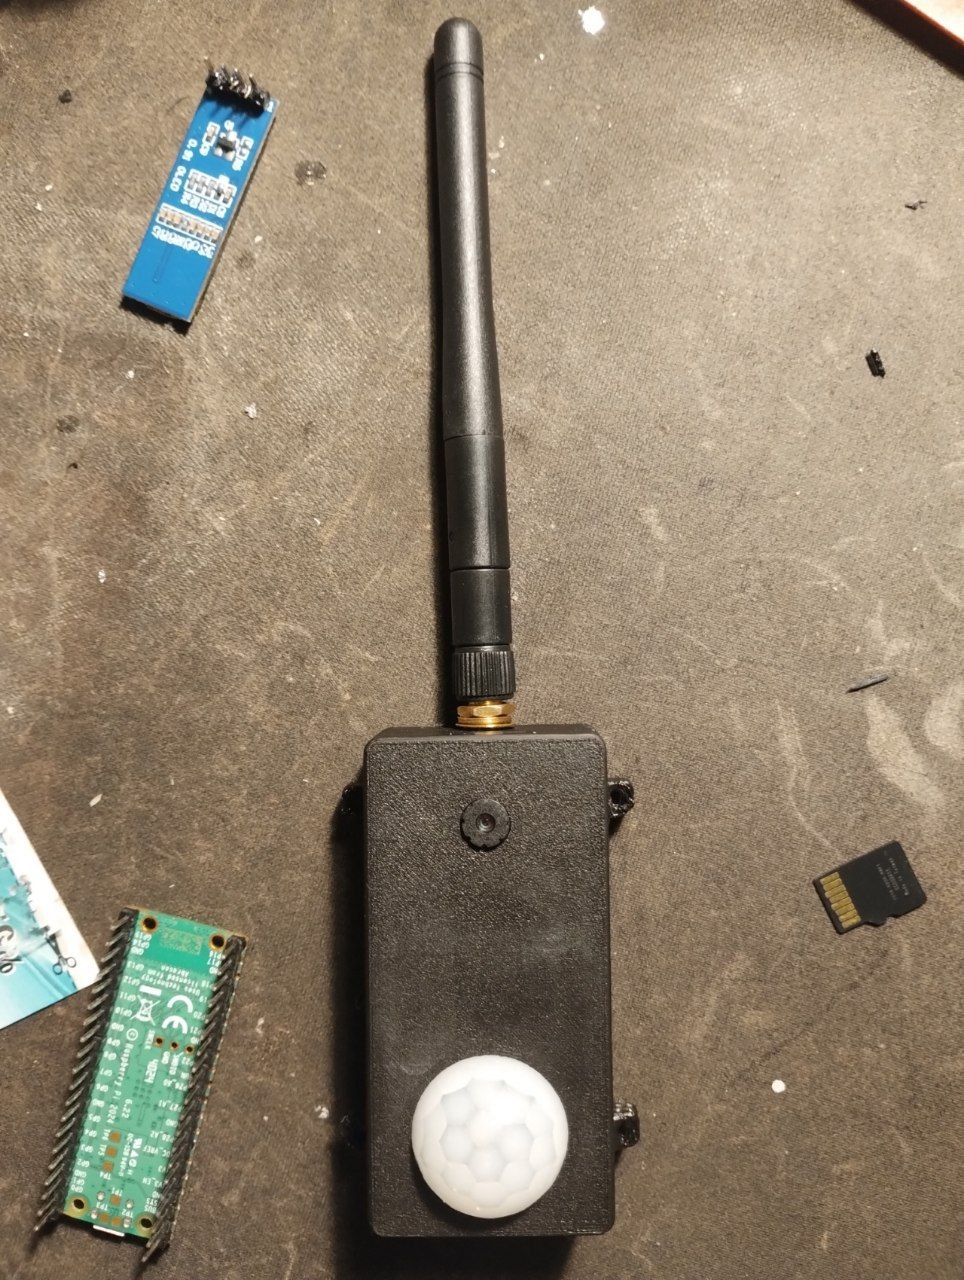
\includegraphics[width=0.5\textwidth]{img/nodoEnsamblado.jpg}
  \caption{Nodo de cámara completamente ensamblado.}
  \label{fig:hardware-ensamblado}
\end{figure}

\newpage
\subsection{Entorno de software y servicios}

A nivel de software, los dispositivos operaron con el firmware desarrollado sobre ESP-IDF (versión 5) y la biblioteca ESP-MESH-LITE.

El backend se alojó en un entorno Linux, utilizando contenedores Docker para estandarizar la ejecución de los servicios. La configuración incluyó una base de datos PostgreSQL, el servicio de inferencia de \gls{speciesnet} servido mediante LitServe, y el \Gls{telegram-bot} encargado de gestionar las notificaciones para los usuarios.

\begin{lstlisting}[caption={Estadísticas de contenedores Docker corriendo.}, label=lst:docker-stats, numbers=none, emphstyle=\bfseries, basicstyle=\ttfamily]
NAME                        CPU %     MEM USAGE  MEM %     PIDS
server-project-bot          0.00%     21.93MiB   0.14%     3
server-project-web          0.40%     56.11MiB   0.36%     4
server-project-db           6.07%     20.51MiB   0.13%     6
server-project-speciesnet   0.33%     69.67MiB   0.44%     1
\end{lstlisting}

El Listado~\ref{lst:log-servidor} muestra un extracto representativo de la salida combinada de los contenedores durante la operación normal del sistema. En él se identifican cuatro tipos de eventos concurrentes:

\begin{itemize}
  \item \textbf{bot-1}: Consultas periódicas a la API de Telegram mediante \texttt{getUpdates} (\textit{long polling}), verificando la existencia de nuevos mensajes o interacciones de los usuarios.
  \item \textbf{speciesnet-1}: Verificaciones periódicas de salud del servicio (\texttt{GET /health}) y peticiones de inferencia (\texttt{POST /predict}) disparadas por la llegada de imágenes desde los nodos.
  \item \textbf{web-1}: Recepción de imágenes cargadas por los nodos de cámara a través de la API REST (\texttt{POST /upload/}), cuya IP de origen corresponde a la del nodo raíz en la red local.
  \item \textbf{db-1}: Operaciones internas de PostgreSQL (\textit{checkpoint}), que persisten periódicamente los datos modificados en memoria hacia el almacenamiento permanente.
\end{itemize}

Se observa la correlación temporal entre los eventos de carga (\texttt{web-1 POST /upload/}) y las predicciones subsiguientes (\texttt{speciesnet-1 POST /predict}), lo cual evidencia el encadenamiento correcto del pipeline de procesamiento: cada imagen recibida por el servicio web es enviada automáticamente al modelo de inferencia para su análisis.

\begin{lstlisting}[caption={Extracto de los registros del servidor durante la recepción y procesamiento de imágenes.}, label=lst:log-servidor, numbers=none, basicstyle=\ttfamily\scriptsize, breaklines=true]
bot-1         | INFO:httpx:HTTP Request: POST
                https://api.telegram.org/bot<TOKEN>/getUpdates
                "HTTP/1.1 200 OK"
speciesnet-1  | INFO: 127.0.0.1:35346
                - "GET /health HTTP/1.1" 200 OK
bot-1         | INFO:httpx:HTTP Request: POST
                https://api.telegram.org/bot<TOKEN>/getUpdates
                "HTTP/1.1 200 OK"
speciesnet-1  | INFO: 172.18.0.4:50210
                - "POST /predict HTTP/1.1" 200 OK
web-1         | 192.168.1.41:49356
                - "POST /upload/ HTTP/1.1" 200
speciesnet-1  | INFO: 127.0.0.1:36684
                - "GET /health HTTP/1.1" 200 OK
speciesnet-1  | INFO: 172.18.0.4:33932
                - "POST /predict HTTP/1.1" 200 OK
web-1         | 192.168.1.41:49357
                - "POST /upload/ HTTP/1.1" 200
db-1          | 2026-04-28 20:26:56.881 UTC [28] LOG:
                checkpoint starting: time
db-1          | 2026-04-28 20:26:57.196 UTC [28] LOG:
                checkpoint complete: wrote 4 buffers (0.0%)
speciesnet-1  | INFO: 172.18.0.4:58278
                - "POST /predict HTTP/1.1" 200 OK
web-1         | 192.168.1.41:49358
                - "POST /upload/ HTTP/1.1" 200
\end{lstlisting}

\section{Pruebas de laboratorio}

Las pruebas de laboratorio se realizaron en condiciones controladas de
interior, verificando el funcionamiento individual de cada componente
antes de la integración.

\subsection{Pruebas de captura de imagen}

Se verificó la correcta captura de imágenes por parte del módulo OV2640, evaluando la inicialización adecuada de la cámara y la calidad fotográfica a diferentes niveles de compresión. Se determinó que el tamaño de archivo resultante oscila entre \qty{30}{KB} y \qty{35}{KB} para una resolución de $640\times480$ píxeles, analizando a su vez el tiempo necesario para completar el ciclo de captura y compresión en hardware.

\begin{figure}[htbp]
  \centering
  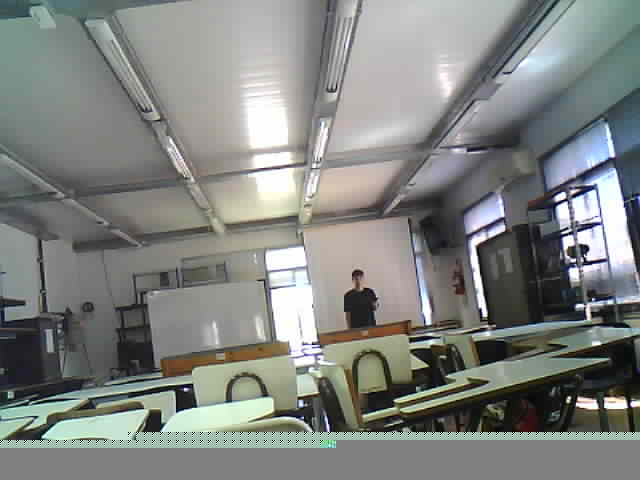
\includegraphics[width=0.6\textwidth]{img/imagenCapturadaNodo.png}
  \caption{Ejemplo de imagen capturada por un nodo de cámara.}
  \label{fig:ejemplo-captura}
\end{figure}

\subsection{Pruebas de conexión a la red mesh}

Se verificó el proceso de asociación de nuevos nodos a la topología de la red mediante el registro de eventos en la consola serial. El Listado~\ref{lst:log-conexion} ilustra la secuencia cuando un nuevo nodo de cámara se asocia exitosamente al nodo raíz. Como se observa en el extracto, el nodo ingresa a la red (identificado con la dirección MAC \texttt{44:1d:64:f3:c2:70}), recibe una dirección IP (\texttt{192.168.5.2}) provista por el servidor DHCP interno y, subsecuentemente, el nodo raíz actualiza su estado interno reflejando el incremento en su contador de nodos hijos directos.

\begin{lstlisting}[caption={Registro de consola mostrando la conexión de un nuevo nodo a la red mesh.}, label=lst:log-conexion, numbers=none, basicstyle=\ttfamily\scriptsize]
I (31313) root_node: ========================
I (41297) root_node: === ROOT NODE STATUS ===
I (41297) root_node: Channel: 2 | Level: 1 (root)
I (41298) root_node: Self MAC: 00:70:07:25:c3:b8
I (41299) root_node: Router BSSID: 48:96:d9:70:a9:4a | RSSI: -36 dBm
I (41305) root_node: Direct children: 0
I (41309) root_node: Free heap: 199396 bytes
I (41313) root_node: ========================
I (43157) wifi:new:<2,1>, old:<2,1>, ap:<2,1>, sta:<2,1>, prof:1, snd_ch_cfg:0x0
I (43158) wifi:station: 44:1d:64:f3:c2:70 join, AID=1, bgn, 40U
I (43190) bridge_wifi: STA Connecting to the AP again...
I (43243) esp_netif_lwip: DHCP server assigned IP to a client, IP is: 192.168.5.2
I (44340) wifi:<ba-add>idx:2 (ifx:1, 44:1d:64:f3:c2:70), tid:0, ssn:0, winSize:64
I (51297) root_node: === ROOT NODE STATUS ===
I (51298) root_node: Channel: 2 | Level: 1 (root)
I (51298) root_node: Self MAC: 00:70:07:25:c3:b8
I (51299) root_node: Router BSSID: 48:96:d9:70:a9:4a | RSSI: -36 dBm
I (51305) root_node: Direct children: 1
I (51309) root_node: Free heap: 196824 bytes
I (51313) root_node:   Child[0]: 44:1d:64:f3:c2:70
I (51317) root_node: ========================
\end{lstlisting}

De manera complementaria, el Listado~\ref{lst:log-desconexion} documenta el proceso inverso: la desconexión de un nodo hijo de la red mesh. En el extracto se observa que el nodo raíz reporta inicialmente un hijo directo (\texttt{Direct children: 1}). Segundos después, la capa Wi-Fi detecta la inactividad del nodo hijo mediante un temporizador interno (\texttt{inactive timer}), registrando su salida con \texttt{reason = 4} (desasociación por inactividad). En el siguiente ciclo de reporte de estado ---configurado con un intervalo de \qty{10}{s}--- el nodo raíz refleja la actualización: \texttt{Direct children: 0}, acompañada de la liberación de memoria heap que ocupaba la entrada en la tabla de ruteo.

\begin{lstlisting}[caption={Registro de consola mostrando la desconexión de un nodo de la red mesh.}, label=lst:log-desconexion, numbers=none, basicstyle=\ttfamily\scriptsize]
I (261297) root_node: === ROOT NODE STATUS ===
I (261298) root_node: Channel: 2 | Level: 1 (root)
I (261298) root_node: Self MAC: 00:70:07:25:c3:b8
I (261299) root_node: Router BSSID: 48:96:d9:70:a9:4a | RSSI: -31 dBm
I (261306) root_node: Direct children: 1
I (261309) root_node: Free heap: 196728 bytes
I (261313) root_node:   Child[0]: 44:1d:64:f3:c2:70
I (261318) root_node: ========================
W (267153) wifi:inactive timer: now=fe17b48 last_rx=c488fba
         diff=ebc1, aid[1]44:1d:64:f3:c2:70 leave
I (267177) wifi:station: 44:1d:64:f3:c2:70 leave,
         AID = 1, reason = 4
I (271297) root_node: === ROOT NODE STATUS ===
I (271298) root_node: Channel: 2 | Level: 1 (root)
I (271298) root_node: Self MAC: 00:70:07:25:c3:b8
I (271299) root_node: Router BSSID: 48:96:d9:70:a9:4a | RSSI: -33 dBm
I (271306) root_node: Direct children: 0
I (271309) root_node: Free heap: 198980 bytes
I (271313) root_node: ========================
\end{lstlisting}

\subsection{Pruebas de transmisión mesh}

Se verificó la transmisión de imágenes a través de la red \gls{mesh}, comprobando la transferencia exitosa de las cargas útiles completas. Adicionalmente, se evaluó el tiempo de transmisión desde el nodo origen hasta el servidor y se observó el comportamiento del mecanismo de recuperación ante pérdidas de conectividad temporales. Como se detalla en la Figura~\ref{fig:log-transmision}, las marcas de tiempo (en milisegundos) provistas por el framework en cada línea del registro permiten calcular con precisión la demora de cada etapa del proceso. Por ejemplo, al sustraer el tiempo de inicio de la petición HTTP del tiempo de recepción de la respuesta exitosa, se evidencia un tiempo de envío en la red local inferior a medio segundo (aproximadamente \qty{463}{ms} para una carga útil de \qty{12.9}{KB}). Asimismo, el ciclo operativo completo del nodo —desde la detección de movimiento en el sensor hasta la confirmación de la carga al servidor— toma apenas \qty{1.27}{s}.

% TODO: Agregar screenshot del log de transmisión
\begin{figure}[htbp]
  \centering
  \includegraphics[width=\textwidth]{img/logEnvioImagen.png}
  \caption{Log de transmisión de imagen a través de la red mesh.}
  \label{fig:log-transmision}
\end{figure}

\subsection{Pruebas del sistema de clasificación}

Se evaluó el pipeline de detección y clasificación utilizando imágenes de prueba, verificando la capacidad del modelo para identificar correctamente animales, personas y vehículos. Durante este proceso se comprobó la precisión gráfica de las \glspl{bounding-box}, la exactitud en la \gls{clasificacion-taxonomica} de la fauna detectada y el tiempo de inferencia requerido para procesar cada captura.

\begin{figure}[htbp]
  \centering
  \begin{subfigure}[b]{0.48\textwidth}
    \centering
    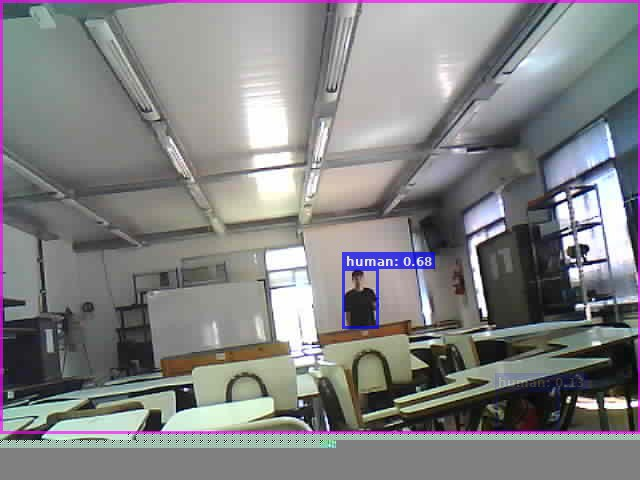
\includegraphics[width=\textwidth]{img/imagenProcesada.png}
    \caption{}
  \end{subfigure}
  \hfill
  \begin{subfigure}[b]{0.48\textwidth}
    \centering
    \includegraphics[width=\textwidth]{img/imgLab1.png}
    \caption{}
  \end{subfigure}

  \vspace{0.5cm}

  \begin{subfigure}[b]{0.48\textwidth}
    \centering
    \includegraphics[width=\textwidth]{img/imgLab2.png}
    \caption{}
  \end{subfigure}
  \hfill
  \begin{subfigure}[b]{0.48\textwidth}
    \centering
    \includegraphics[width=\textwidth]{img/imgLab3.png}
    \caption{}
  \end{subfigure}
  \caption{Ejemplo de imagen procesada por el sistema de detección en entorno de laboratorio.}
  \label{fig:ejemplo-deteccion}
\end{figure}

\newpage
\subsection{Pruebas del panel de monitoreo web}

Se verificó el correcto funcionamiento del panel de monitoreo web, el cual permite visualizar las imágenes capturadas por los nodos de cámara, así como la información de detecciones y clasificaciones.

\begin{figure}[htbp]
  \centering
  \includegraphics[width=\textwidth]{img/panelweb1.png}
  % \fbox{\parbox{0.9\textwidth}{\centering\vspace{2cm}
  %     [Screenshot del panel de monitoreo web]
  % \vspace{2cm}}}
  \caption{Panel de monitoreo web con imágenes capturadas por los nodos de cámara.}
  \label{fig:panel-web}
\end{figure}

\subsection{Pruebas del sistema de alertas}

Se verificó el funcionamiento del bot de Telegram:

\begin{itemize}
  \item Recepción correcta de notificaciones
  \item Envío de imagen original y anotada
  \item Información de detecciones y clasificaciones
  \item Tiempo desde captura hasta notificación
\end{itemize}

\begin{figure}[htbp]
  \centering
  \includegraphics[width=0.5\textwidth]{img/notificacionTelegramLab.png}
  \caption{Notificación recibida en Telegram con resultados de detección.}
  \label{fig:telegram-notificacion}
\end{figure}

\newpage

\subsection{Pruebas de retroalimentación interactiva (\textit{Human-in-the-loop})}

Se evaluó el mecanismo de corrección manual integrado entre el bot de Telegram y el servidor web. Para ello, se partió de una clasificación inicial errónea generada por el modelo (Figura~\ref{fig:hitl-1}). A través de la interfaz del bot, el usuario indicó que la clasificación no era correcta (Figura~\ref{fig:hitl-2}) y seleccionó la etiqueta adecuada (\textit{human}) desde la lista de predicciones alternativas sugeridas (Figura~\ref{fig:hitl-3}). Una vez confirmada la selección, el sistema actualizó el registro en la base de datos, reflejando inmediatamente el resultado corregido y marcando el evento como auditado por el usuario en el panel de monitoreo web (Figura~\ref{fig:hitl-4}).

\begin{figure}[htbp]
  \centering
  \includegraphics[width=0.8\textwidth]{img/clasificacionErroneaAntes.png}
  \caption{Clasificación original errónea en el frontend.}
  \label{fig:hitl-1}
\end{figure}

\begin{figure}[htbp]
  \centering
  \includegraphics[width=0.8\textwidth]{img/seleccionClasificacionErronea.png}
  \caption{Notificación y validación en el bot de Telegram.}
  \label{fig:hitl-2}
\end{figure}

\begin{figure}[htbp]
  \centering
  \includegraphics[width=0.8\textwidth]{img/seleccionHuman.png}
  \caption{Selección de la etiqueta correcta por el usuario.}
  \label{fig:hitl-3}
\end{figure}

\begin{figure}[htbp]
  \centering
  \includegraphics[width=0.8\textwidth]{img/clasificacionCorregida.png}
  \caption{Resultado final actualizado en el frontend.}
  \label{fig:hitl-4}
\end{figure}

\newpage
\section{Pruebas de campo}

\begin{figure}[htbp]
  \centering
  \includegraphics[width=0.85\textwidth]{img/entrada_jardin.jpg}
  \caption{Ingreso al jardín botánico, lugar donde se realizaron las pruebas de campo.}
  \label{fig:entrada-jardin}
\end{figure}

\subsection{Configuración del entorno}

Las pruebas de campo se realizaron en un entorno exterior, instalando
los nodos de cámara en ubicaciones representativas de un despliegue real.

\begin{figure}[htbp]
  \centering
  \begin{subfigure}[b]{0.48\textwidth}
    \centering
    \includegraphics[height=8cm]{img/nodoCampo1Lejos.jpg}
    \caption{Vista general}
    \label{fig:despliegue-campo-1-lejos}
  \end{subfigure}
  \hfill
  \begin{subfigure}[b]{0.48\textwidth}
    \centering
    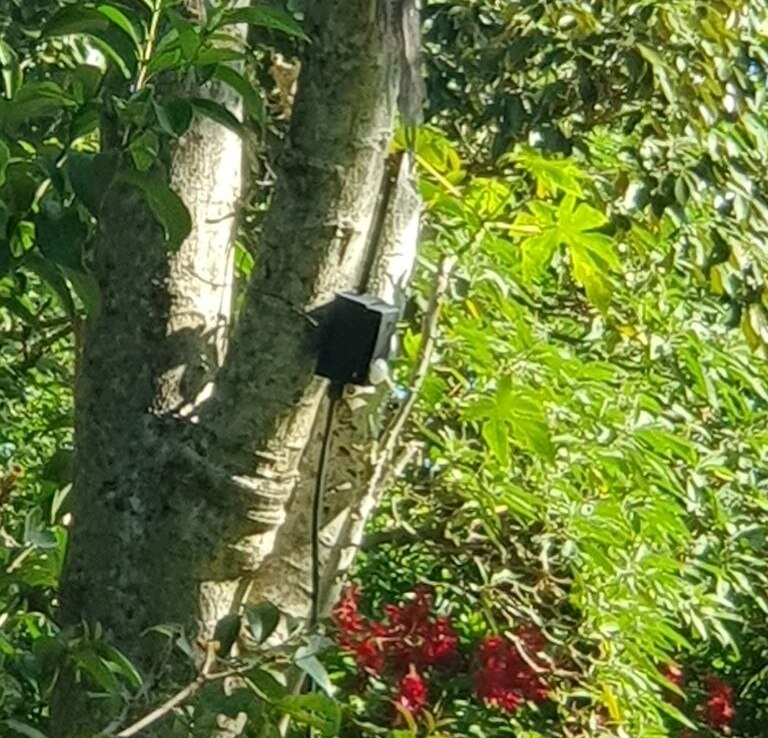
\includegraphics[height=8cm]{img/nodoCampo1.jpg}
    \caption{Acercamiento con zoom digital 10x}
    \label{fig:despliegue-campo-1-zoom}
  \end{subfigure}
  \caption{Primer nodo de cámara desplegado en el entorno exterior.}
  \label{fig:despliegue-campo-1}
\end{figure}

\begin{figure}[htbp]
  \centering
  \begin{subfigure}[b]{0.48\textwidth}
    \centering
    \includegraphics[height=10cm]{img/nodoCampo2Lejos.jpg}
    \caption{Vista general}
    \label{fig:despliegue-campo-2-lejos}
  \end{subfigure}
  \hfill
  \begin{subfigure}[b]{0.48\textwidth}
    \centering
    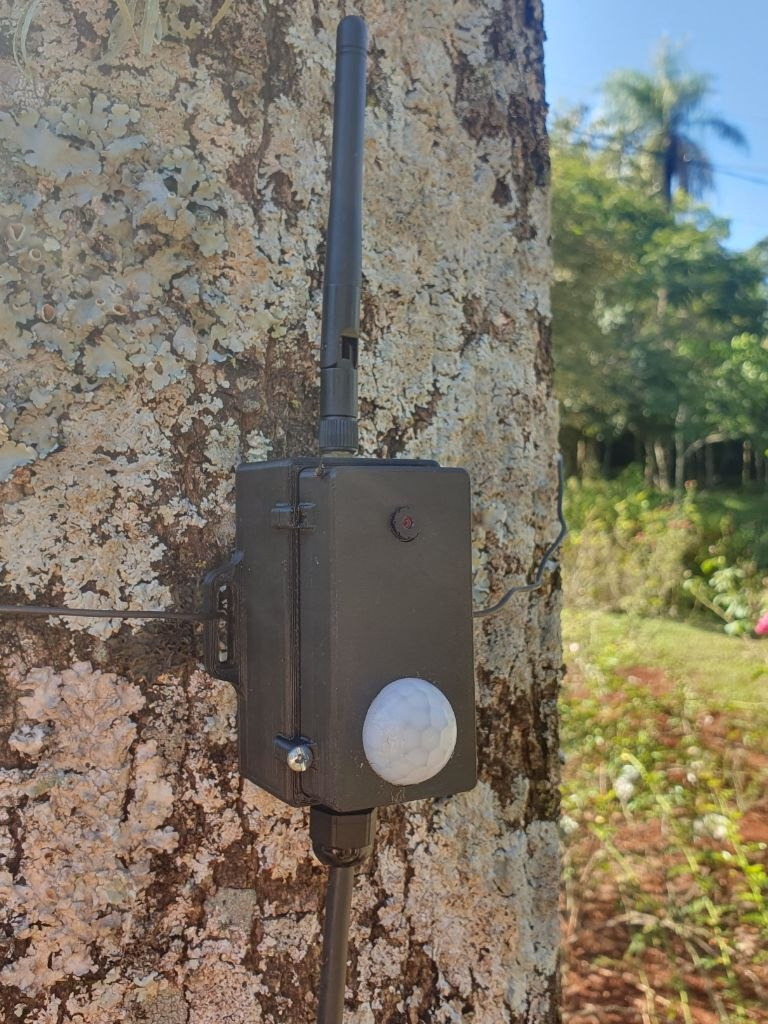
\includegraphics[height=10cm]{img/nodoCampo2.jpg}
    \caption{Primer plano del nodo}
    \label{fig:despliegue-campo-2-cerca}
  \end{subfigure}
  \caption{Segundo nodo de cámara desplegado en el entorno exterior.}
  \label{fig:despliegue-campo-2}
\end{figure}

\begin{figure}[htbp]
  \centering
  \begin{subfigure}[b]{0.48\textwidth}
    \centering
    \includegraphics[height=10cm]{img/nodoCampo3b.jpg}
    \caption{Vista general}
    \label{fig:despliegue-campo-3-a}
  \end{subfigure}
  \hfill
  \begin{subfigure}[b]{0.48\textwidth}
    \centering
    \includegraphics[height=10cm]{img/nodoCampo3a.jpg}
    \caption{Ángulo alternativo}
    \label{fig:despliegue-campo-3-b}
  \end{subfigure}
  \caption{Tercer nodo de cámara desplegado en el entorno exterior}
  \label{fig:despliegue-campo-3}
\end{figure}

\subsection{Condiciones de las pruebas}

Las pruebas de campo se realizaron bajo las siguientes condiciones:

% TODO: Revisar datos
\begin{itemize}
  \item Duración: 5 horas de operación continua
  \item Condiciones climáticas: soleado
  \item Número de nodos desplegados: 3
  \item Distancia entre nodos: 15 metros
  \item Distancia al router Wi-Fi: 15 metros
\end{itemize}

\newpage
\subsection{Resultados obtenidos}

Durante las pruebas de campo se registraron los siguientes resultados.

\subsubsection{Desempeño del modelo de inferencia}

El desempeño del modelo se evaluó sobre un conjunto de 94 imágenes de prueba
capturadas en condiciones de campo. Para cada imagen, la salida
del servicio de inferencia fue contrastada con la etiqueta real, construyéndose
las matrices de confusión que se presentan en la Figura~\ref{fig:matrices-confusion}.

\paragraph{Lógica de umbrales de detección.}
Antes de interpretar las matrices, es necesario comprender la lógica de decisión
que el sistema aplica sobre la salida de \gls{speciesnet}. El modelo produce dos
resultados independientes para cada imagen: un puntaje de detección
(\textit{bounding box confidence}), que indica la confianza de que exista algún
objeto en la escena, y una clasificación de especie, que categoriza dicho
objeto. El sistema combina ambos resultados mediante tres umbrales configurables
para decidir si la imagen debe enviarse al Telegram:

\begin{description}
  \item[\texttt{DETECTION\_HIGH} = 0{,}80:]
    Si la confianza de detección supera el 80\%, la imagen se acepta y transmite
    de forma inmediata, independientemente de lo que indique el clasificador de
    especies. Este umbral cubre los casos de alta certeza donde el modelo no tiene
    dudas sobre la presencia de un objeto.

  \item[\texttt{DETECTION\_MID} = 0{,}50:]
    Si la confianza de detección se encuentra entre el 50\% y el 80\%, pero el
    clasificador señala que la imagen está vacía (\textit{blank}), el sistema opta
    por transmitirla igualmente. Esta regla está diseñada para evitar la pérdida
    de detecciones de animales pequeños o lejanos, cuya silueta puede no ser lo
    suficientemente distintiva para el clasificador, pero sí activa el detector
    de objetos.

    \item[\texttt{DETECTION\_LOW} = 0{,}30:]
    Si la confianza de detección es inferior al 30\% y el clasificador también
    indica imagen vacía, la imagen se descarta. En este caso el sistema asume que
    se trata de un probable falso positivo del sensor de movimiento, como el
    balanceo de ramas por el viento.
\end{description}

Esta lógica de tres niveles permite al sistema operar con una política de
sesgo hacia la sensibilidad: ante la duda, se prefiere transmitir la imagen y
delegar la decisión final al operador humano, reduciendo el riesgo de perder
eventos reales a costa de aceptar algunas falsas alarmas.

\paragraph{Detección binaria.}
Teniendo en cuenta la lógica anterior, la Figura~\ref{fig:confusion-binaria}
presenta la matriz de confusión para la tarea de detección binaria, donde el
modelo distingue entre imágenes que contienen algún objeto de interés
(\textit{Positivo}: fauna, personas o vehículos) e imágenes sin objeto
(\textit{Negativo}: blanco). Los resultados se resumen en la
Tabla~\ref{tab:metricas-binarias}.

\newpage
\begin{table}[htbp]
  \centering
  \caption{Métricas de clasificación binaria del modelo de inferencia.}
  \label{tab:metricas-binarias}
  \begin{tblr}{
      colspec = {X[l] r},
      row{1} = {font=\bfseries},
      hlines,
    }
    Métrica      & Valor  \\
    Verdaderos Positivos (TP)  & 30     \\
    Verdaderos Negativos (TN)  & 43     \\
    Falsos Positivos (FP)      & 8      \\
    Falsos Negativos (FN)      & 13     \\
    Exactitud (\textit{Accuracy})   & 77{,}7\% \\
    Precisión (\textit{Precision})  & 78{,}9\% \\
    Exhaustividad (\textit{Recall}) & 69{,}8\% \\
  \end{tblr}
\end{table}

El modelo demostró una exactitud general del 77{,}7\%. Se registraron 8 falsos
positivos (imágenes en blanco clasificadas erróneamente como positivas) y
13 falsos negativos (imágenes con objetos reales que el modelo no detectó).
En el contexto del sistema propuesto, los falsos negativos representan el error
más crítico, ya que implican eventos de interés no reportados. Sin embargo, dado
que el objetivo principal no es alcanzar precisión perfecta en la inferencia
inicial, sino integrar el modelo como asistente dentro de un enfoque
\textit{Human-in-the-loop}, ambos tipos de error son tolerados. A futuro, los
datos corregidos por el usuario podrán emplearse para aplicar técnicas de
\textit{fine-tuning} o \textit{transfer learning} sobre el modelo base.

\paragraph{Clasificación multiclase.}
La Figura~\ref{fig:confusion-multiclase} presenta la matriz de confusión para
la tarea de clasificación multiclase, donde cada detección positiva es asignada
a una de las cuatro categorías: \textit{blanco}, \textit{animales},
\textit{personas} o \textit{vehículos}. El análisis por clase revela
comportamientos diferenciados:

\begin{itemize}
  \item \textbf{Blanco:} 43 de 51 muestras correctamente clasificadas
    (Recall = 84{,}3\%). Los 8 errores restantes corresponden a imágenes en
    blanco clasificadas como \textit{animales} (6) y \textit{personas} (2).
  \item \textbf{Animales:} 9 de 17 muestras correctamente clasificadas
    (Recall = 52{,}9\%). Es la clase con menor desempeño: 8 imágenes reales de
    animales fueron predichas como \textit{blanco}, lo que refleja la dificultad
    inherente de detectar fauna silvestre en entornos naturales con variaciones
    de iluminación y tamaño del sujeto.
  \item \textbf{Personas:} 17 de 22 muestras correctamente clasificadas
    (Recall = 77{,}3\%), con 5 casos confundidos con \textit{blanco}. La
    precisión es elevada (89{,}5\%), lo que indica que cuando el modelo predice
    una persona, rara vez se equivoca.
  \item \textbf{Vehículos:} 2 de 2 muestras correctamente clasificadas
    (Recall = 100\%, Precision = 100\%), aunque el tamaño reducido de esta clase
    limita la generalización de este resultado.
\end{itemize}

El principal vector de error del modelo es la confusión entre la clase
\textit{animales} y \textit{blanco}, consistente con la naturaleza del conjunto
de datos de prueba, donde la fauna de pequeño y mediano porte puede confundirse
fácilmente con el fondo en imágenes de cámara trampa. No obstante, el servicio
de inferencia opera correctamente de forma integrada al sistema y es capaz de
detectar los eventos de interés definidos en los objetivos del trabajo.

\begin{figure}[htbp]
  \centering
  \begin{subfigure}[b]{0.48\textwidth}
    \centering
    \includegraphics[width=\textwidth]{img/confusion_matrix_binary.png}
    \caption{Detección binaria (Positivo vs.\ Negativo).}
    \label{fig:confusion-binaria}
  \end{subfigure}
  \hfill
  \begin{subfigure}[b]{0.48\textwidth}
    \centering
    \includegraphics[width=\textwidth]{img/confusion_matrix.png}
    \caption{Clasificación multiclase.}
    \label{fig:confusion-multiclase}
  \end{subfigure}
  \caption{Matrices de confusión obtenidas con el conjunto de imágenes de prueba.}
  \label{fig:matrices-confusion}
\end{figure}

\subsubsection{Detección de eventos en campo}

Además de la evaluación cuantitativa, las pruebas de campo demostraron la eficacia
del sistema como herramienta de seguridad y vigilancia perimetral. La
Figura~\ref{fig:ejemplos-deteccion-campo} ilustra detecciones exitosas de intrusos
y vehículos no autorizados en el predio.

\begin{figure}[htbp]
  \centering
  \begin{subfigure}[b]{0.48\textwidth}
    \centering
    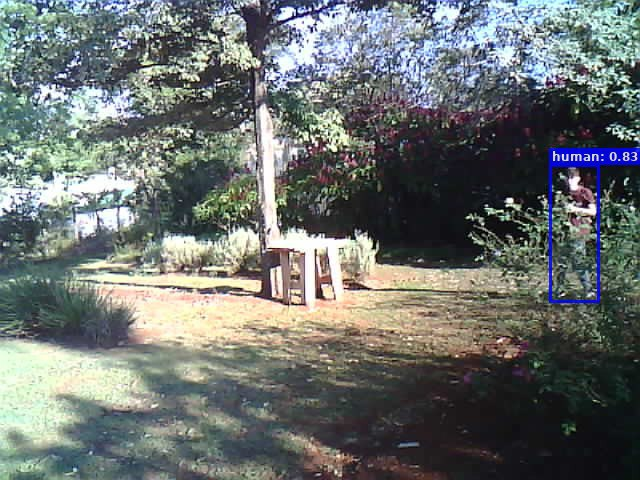
\includegraphics[width=\textwidth]{img/capturaIntrusoProcesada.png}
    \caption{Detección de intrusos (personas).}
    \label{fig:deteccion-intruso}
  \end{subfigure}
  \hfill
  \begin{subfigure}[b]{0.48\textwidth}
    \centering
    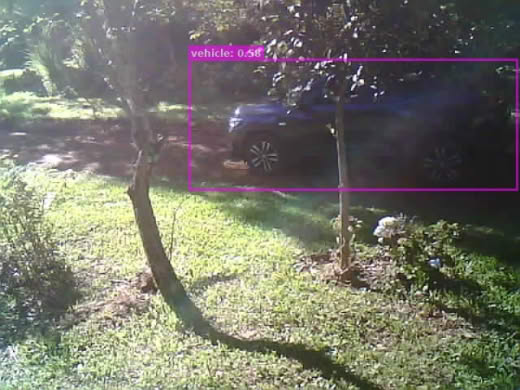
\includegraphics[width=\textwidth]{img/capturaAutoProcesada.jpg}
    \caption{Detección de vehículos.}
    \label{fig:deteccion-auto}
  \end{subfigure}
  \caption{Versatilidad del modelo demostrada durante las pruebas de campo.}
  \label{fig:ejemplos-deteccion-campo}
\end{figure}

La Figura~\ref{fig:deteccion-ave-campo} presenta un caso particularmente relevante: la detección de un ave silvestre de pequeño porte alimentándose en el área monitoreada. El sistema logró identificar al animal con valores de confianza de 0.74 y 0.90 en capturas sucesivas, demostrando la capacidad de detectar fauna de reducido tamaño corporal en condiciones reales de campo.

\begin{figure}[htbp]
  \centering
  \begin{subfigure}[b]{0.48\textwidth}
    \centering
    \includegraphics[width=\textwidth]{img/pajarito1.png}
    \caption{Primera detección (confianza: 0.74).}
    \label{fig:deteccion-ave-1}
  \end{subfigure}
  \hfill
  \begin{subfigure}[b]{0.48\textwidth}
    \centering
    \includegraphics[width=\textwidth]{img/pajarito2.png}
    \caption{Segunda detección (confianza: 0.90).}
    \label{fig:deteccion-ave-2}
  \end{subfigure}
  \caption{Detección de ave silvestre durante las pruebas de campo.}
  \label{fig:deteccion-ave-campo}
\end{figure}

Asimismo, la Figura~\ref{fig:deteccion-gato-campo} muestra la detección de un gato doméstico que ingresó al área monitoreada. El modelo lo identificó correctamente como animal con un valor de confianza de 0.96, evidenciando la capacidad del sistema para detectar fauna de porte mediano incluso en condiciones de contraluz.

\begin{figure}[htbp]
  \centering
  \includegraphics[width=0.6\textwidth]{img/gato.png}
  \caption{Detección de un gato doméstico durante las pruebas de campo (confianza: 0.96).}
  \label{fig:deteccion-gato-campo}
\end{figure}

\newpage
\section{Métricas de rendimiento de red}

\subsection{Latencia de transmisión}

La latencia de extremo a extremo del sistema —definida como el tiempo transcurrido desde la captura de la imagen en el nodo de cámara hasta su completa recepción y disponibilidad en el servidor— está supeditada a la interacción de múltiples factores:

\begin{itemize}
  \item \textbf{Calidad de la señal Wi-Fi:} El nivel de potencia de la señal recibida (RSSI) entre cada nodo y su respectivo padre influye directamente en la tasa de transmisión efectiva y en la probabilidad de requerir retransmisiones por pérdida de paquetes.
  \item \textbf{Ancho de banda de salida:} La capacidad de enlace proporcionada por el punto de acceso al que se conecta el nodo raíz actúa como el principal cuello de botella hacia internet.
  \item \textbf{Profundidad de la topología:} Cada salto adicional en la estructura de la red de árbol introduce retardos intrínsecos, dado que la carga útil debe ser procesada y reenviada en la capa de red por cada nodo intermedio.
  \item \textbf{Tamaño de la carga útil:} Las imágenes comprimidas en formato \gls{jpeg} presentan tamaños que oscilan entre \qty{30}{KB} y \qty{35}{KB}, un volumen de datos considerable para enlaces Wi-Fi de bajo consumo en configuraciones en malla.
\end{itemize}

Para propósitos analíticos, es fundamental distinguir entre la latencia en condiciones ideales de red local (LAN) y la latencia de extremo a extremo experimentada en entornos de campo. En las pruebas de laboratorio, con el servidor operando en la misma subred que el nodo raíz, las métricas extraídas de los registros del microcontrolador indicaron tiempos sumamente reducidos. El tiempo puro de transmisión HTTP para una carga útil típica de \qty{12.9}{KB} fue de aproximadamente \qty{463}{ms}, resultando en un ciclo operativo completo en el nodo —desde la detección de movimiento hasta el fin de la carga— de tan solo \qty{1.27}{s}.

En contraste, para el desarrollo de las pruebas de campo, el nodo raíz se vinculó a internet mediante un punto de acceso móvil (\textit{hotspot}) provisto por un teléfono celular. Durante las sesiones, se experimentó una cobertura deficiente de señal de telefonía móvil en el lugar de despliegue, lo cual introdujo un grado de inestabilidad y limitó el ancho de banda ascendente, impactando directamente en los tiempos de respuesta. Una conexión con mejor cobertura celular o el uso de un enrutador dedicado ofrecería un canal más estable, lo cual redundaría en una mejora significativa sobre los tiempos observados.

Los tiempos documentados en la Tabla~\ref{tab:latencia} corresponden a valores empíricos aproximados obtenidos durante las sesiones de campo. Ante la ausencia de un conjunto de datos extenso y sistemático, estas métricas se presentan como indicadores del comportamiento operativo general bajo las condiciones de prueba detalladas.

\newpage
\begin{table}[htbp]
  \centering
  \caption{Latencia de transmisión observada (conexión vía \textit{hotspot} celular).}
  \label{tab:latencia}
  \begin{tabular}{lc}
    \hline
    \textbf{Métrica aproximada} & \textbf{Valor} \\
    \hline
    Latencia mínima observada   & 20 \unit{s}   \\
    Latencia promedio estimada  & 40 \unit{s}   \\
    Latencia máxima observada   & 60 \unit{s}   \\
    Desviación estándar         & $\approx$ 10 \unit{s}   \\
    \hline
  \end{tabular}
\end{table}

\subsection{Distancia máxima entre nodos}

Con el propósito de caracterizar el alcance efectivo de los módulos de comunicación, se efectuaron pruebas empíricas para determinar la distancia máxima a la cual dos nodos pueden sostener un enlace operativo. La metodología consistió en establecer una conexión inicial exitosa y, posteriormente, desplazar físicamente uno de los nodos de forma gradual mientras se monitoreaba el estado de la red a través de la consola serial. El límite de distancia se determinó en el punto donde la degradación de la métrica RSSI provocaba la caída recurrente del enlace y la consecuente imposibilidad de transmitir imágenes.

Los resultados consolidados de estas observaciones se exponen en la Tabla~\ref{tab:distancia}. Si bien el sistema utiliza una antena externa omnidireccional conectada al módulo ESP32-CAM para maximizar el alcance, la propagación en la banda de \qty{2.4}{\giga\hertz} sigue siendo altamente susceptible a la atenuación provocada por obstáculos físicos. En entornos caracterizados por vegetación densa, el rango útil experimentó reducciones considerables en comparación con el escenario ideal de línea de vista directa, un factor crítico a tener en cuenta para la planificación del espaciado entre nodos durante un despliegue real.

Es importante destacar que el alcance útil reportado se refiere específicamente a la transmisión exitosa de imágenes (cargas útiles pesadas de entre \qtyrange{30}{50}{\kilo\byte}). En redes inalámbricas, a medida que la señal se degrada por la distancia y disminuye la relación señal-ruido (SNR), la probabilidad de pérdida de paquetes aumenta. La transmisión de una imagen requiere la fragmentación de los datos en decenas de paquetes (de \qty{1,4}{\kilo\byte}). A bajas tasas de modulación, esto implica tiempos prolongados de ocupación del medio inalámbrico (cientos de milisegundos), lo que expone los datos a mayores interferencias. Si bien a 15-20 metros el envío de un texto simple (un único paquete) sería altamente exitoso, la transmisión de una imagen experimenta una alta tasa de retransmisiones, dado que la probabilidad de éxito de la carga útil completa decae exponencialmente a medida que aumenta el número de fragmentos~\cite{sankarasubramaniam2003energy}. Esto congestiona la red y provoca desconexiones por tiempos de espera excedidos (\textit{timeouts}) en la capa de enrutamiento \gls{mesh}. Por consiguiente, la distancia máxima efectiva se ve fuertemente limitada por el tamaño de la carga útil.

Con el propósito de extender el alcance efectivo entre los nodos, resultaría factible implementar una combinación de estrategias técnicas. Entre ellas se destacan el incremento de la potencia de transmisión (mediante modificaciones en el diseño del hardware o la incorporación de antenas de mayor ganancia), la reducción del umbral mínimo de RSSI en la configuración del firmware, y la minimización del tamaño de las cargas útiles mediante una mayor compresión de las imágenes. No obstante, dado que las distancias operativas obtenidas resultaron suficientes para validar la viabilidad técnica de la topología \gls{mesh} en el escenario propuesto ---cumpliendo así con los objetivos centrales del proyecto---, la implementación de estas optimizaciones fue diferida para ser abordada en trabajos futuros.

\begin{table}[htbp]
  \centering
  \caption{Alcance máximo efectivo observado entre nodos adyacentes.}
  \label{tab:distancia}
  \begin{tabular}{lc}
    \hline
    \textbf{Condición del entorno} & \textbf{Distancia máxima} \\
    \hline
    Línea de vista directa      & 15-18 \unit{m} \\
    Con obstáculos (vegetación) & $\approx$ 12 \unit{m} \\
    Interior (paredes)          & $\approx$ 10 \unit{m} \\
    \hline
  \end{tabular}
\end{table}

\subsection{Estabilidad de la conexión}

La estabilidad de la red mesh durante operación prolongada depende de la interacción de múltiples factores ambientales y de configuración, lo que dificulta su caracterización mediante una única métrica cuantitativa.

Durante las pruebas de campo, se observó que la red mantuvo conectividad operativa de forma estable siempre que se cumplieran dos condiciones: que los nodos dispusieran de carga de batería suficiente y que la calidad de la señal Wi-Fi entre nodos adyacentes fuera adecuada (considerando un umbral mínimo de RSSI de \qty{-75}{dBm}, un parámetro configurable en el firmware).

Si bien existen diversos factores que podrían incidir negativamente en la estabilidad, en las pruebas de campo realizadas no tuvieron un impacto significativo, ya que se seleccionaron entornos con vegetación moderada y condiciones climáticas favorables. Teóricamente, los factores de riesgo que podrían afectar el sistema incluyen:

\begin{itemize}
  \item \textbf{Calidad de señal entre nodos:} La vegetación muy densa y las condiciones climáticas adversas pueden degradar la señal y provocar reconexiones esporádicas. En nuestras pruebas, al contar con ubicaciones favorables, las desconexiones espontáneas resultaron prácticamente nulas.
  \item \textbf{Agotamiento de batería:} Constituye el principal motivo de interrupción. Cuando la tensión del pack desciende por debajo del umbral funcional del regulador, el nodo se apaga de forma definitiva y no se reincorpora a la red hasta ser recargado manualmente.
  \item \textbf{Saturación del punto de acceso:} En escenarios con alta concurrencia de dispositivos conectados al mismo router Wi-Fi, se podrían presentar retardos adicionales en la transmisión de imágenes.
  \item \textbf{Profundidad de la topología:} A mayor cantidad de saltos en la red de árbol, mayor es la probabilidad de que una desconexión en un nodo intermedio afecte a los nodos descendientes.
\end{itemize}

El firmware implementa un mecanismo de verificación periódica de la tabla de ruteo con un intervalo configurado de \qty{60}{s}. Este ciclo determina el tiempo máximo que un nodo tarda en detectar la pérdida de su padre y comenzar el proceso de reasociación a un nodo alternativo, estableciendo así el tiempo de reconexión en el peor caso.

En cuanto a la integridad de las imágenes transmitidas, la arquitectura basada en peticiones HTTP sobre TCP garantiza la entrega confiable a nivel de transporte. Las imágenes que llegaron al servidor se recibieron completas y sin corrupción. Los casos de pérdida correspondieron a situaciones donde el nodo no logró completar la transmisión (por desconexión de la red o agotamiento de batería durante el envío), resultando en imágenes que nunca fueron registradas por el servidor.

\section{Métricas de consumo energético}

\subsection{Consumo promedio del nodo}

Se midió el consumo eléctrico del nodo en diferentes estados de operación:

\begin{table}[htbp]
  \centering
  \caption{Consumo energético por estado de operación.}
  \label{tab:consumo}
  \begin{tabular}{lc}
    \hline
    \textbf{Estado}            & \textbf{Consumo (\unit{mA})} \\
    \hline
    Modo ULP                   & 13                          \\
    Captura y envío de imagen  & 200                          \\
    Consumo promedio           & 180                          \\
    \hline
  \end{tabular}
\end{table}

\begin{figure}[htbp]
  \centering
  \includegraphics[width=0.48\textwidth]{img/consumoULP.jpg}
  \caption{Consumo energético del nodo hoja en modo de ultra bajo consumo (ULP).}
  \label{fig:consumo_ulp}
\end{figure}

\subsection{Autonomía estimada}

La autonomía del nodo depende de la capacidad utilizable del pack de baterías y del consumo promedio ponderado. Es importante distinguir entre la capacidad nominal y la capacidad utilizable: las celdas de iones de litio 18650 no deben descargarse por debajo de \qty{2.5}{V} por celda para preservar su vida útil. En una configuración 2S, esto implica un voltaje mínimo del pack de \qty{5.0}{V}.

Sin embargo, el módulo regulador LM2596 (\gls{buck-converter}) requiere un margen de tensión (\textit{dropout}) de aproximadamente \qty{1.5}{V} por encima de su voltaje de salida (\qty{5}{V}), estableciendo un voltaje mínimo de entrada funcional de \qty{6.5}{V} (equivalente a \qty{3.25}{V} por celda). Cuando la tensión del pack cae por debajo de este umbral, el regulador no puede mantener una salida estable de \qty{5}{V}. Los picos de corriente característicos del ESP32-CAM durante la transmisión Wi-Fi (que pueden superar los \qty{300}{mA} instantáneos) provocan caídas momentáneas en la línea de alimentación, disparando la protección de \textit{brownout} del microcontrolador y reiniciándolo. Este comportamiento fue observado consistentemente durante las pruebas cuando la tensión de entrada al regulador descendía por debajo de \qtyrange{6}{7}{V}.

En consecuencia, la capacidad efectivamente utilizable del pack es inferior a los \qty{3500}{mAh} nominales. Considerando la curva de descarga típica de las celdas 18650~\cite{powar2025discharge18650} y el corte práctico en \qty{3.25}{V} por celda, la capacidad aprovechable se reduce a aproximadamente un \qty{40}{\percent} de la nominal. La Figura~\ref{fig:curva-descarga} ilustra esta curva de descarga de referencia, donde se evidencia la caída pronunciada de tensión una vez superado el \qty{60}{\percent} de la capacidad.

\begin{figure}[htbp]
  \centering
  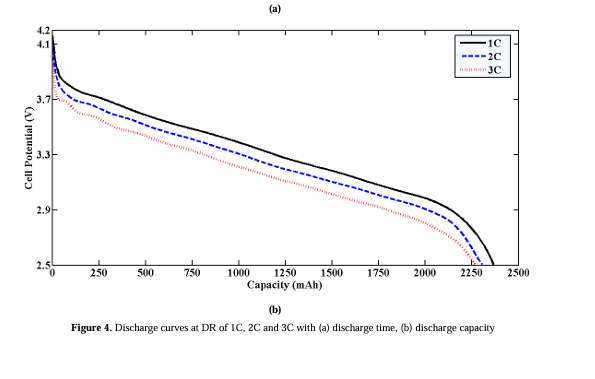
\includegraphics[width=\textwidth]{img/curvaDescargaBateria.png}
  \caption{Curva de descarga típica de celdas 18650\cite{powar2025discharge18650}.}
  \label{fig:curva-descarga}
\end{figure}

\begin{description}
  \item[Capacidad nominal del pack 2S:] \qty{3500}{mAh}
  \item[Capacidad utilizable estimada:] $\approx$ \qty{1400}{mAh} (corte a \qty{6.5}{V} de entrada)
  \item[Consumo promedio (modo Relay):] \qty{180}{mA}
  \item[Autonomía teórica estimada:] $\approx$ \qtyrange{7}{8}{h}
  \item[Autonomía medida en pruebas:] \qty{5}{h}
\end{description}

\section{Análisis de resultados}

Los resultados obtenidos demuestran la viabilidad del sistema propuesto
para el monitoreo de áreas protegidas. A continuación se presenta un
análisis de los principales hallazgos:

\subsection{Cumplimiento de objetivos}

% TODO: Completar análisis de cumplimiento
\begin{description}
  \item[Detección de fauna, personas y vehículos:] El sistema demostró capacidad de detección y clasificación para las tres categorías de interés. El modelo SpeciesNet, ejecutándose en el servidor sin GPU dedicada, procesó correctamente las imágenes capturadas por los nodos, generando detecciones con cuadros delimitadores y clasificación taxonómica para la fauna identificada (Figuras~\ref{fig:ejemplo-deteccion} y \ref{fig:ejemplos-deteccion-campo}).
  \item[Latencia de respuesta:] El tiempo transcurrido desde la detección de movimiento hasta la notificación en Telegram se situó en el orden de los \qty{40}{s} en promedio. Si bien no constituye tiempo real en sentido estricto, representa una mejora de varios órdenes de magnitud frente a las cámaras trampa convencionales, donde el acceso a las imágenes requiere días o semanas de recolección manual.
  \item[Cobertura de red:] La red mesh operó de forma estable con distancias de hasta \qty{18}{m} en línea de vista directa y \qty{12}{m} con vegetación intermedia. Estas distancias, aunque limitadas, son suficientes para un despliegue en cadena con nodos intermedios (Relay).
  \item[Autonomía energética:] Se logró una autonomía medida de \qty{5}{h} en modo Relay (\textit{Light Sleep}), mientras que el modo Leaf (\textit{Deep Sleep} + ULP) demostró un consumo en reposo de \qty{13}{mA}, lo que proyecta autonomías significativamente superiores para nodos que no requieren enrutamiento continuo.
\end{description}

\subsection{Limitaciones observadas}

Las pruebas de campo confirmaron las limitaciones técnicas anticipadas en la Sección~\ref{sec:limitaciones}. En particular, se verificó en la práctica lo siguiente:

\begin{itemize}
  \item El sensor PIR domótico HC-SR501 superó las expectativas iniciales, logrando detectar fauna de pequeño porte como aves que transitaban en las proximidades de la cámara. No obstante, la alta sensibilidad del sensor se tradujo en un número considerable de falsos positivos, generando capturas sin presencia real de fauna o personas en el encuadre.
  \item El alcance efectivo, incluso utilizando una antena externa, se redujo considerablemente en presencia de vegetación, requiriendo distancias entre nodos inferiores a las teóricamente posibles.
  \item Se observaron reinicios por \textit{brownout} cuando la tensión del pack 2S descendió por debajo de \qtyrange{6}{7}{V}, confirmando la insuficiencia del margen de tensión del regulador LM2596 frente a los picos de corriente del módulo Wi-Fi.
  \item La operación del sistema quedó efectivamente restringida a condiciones de luz diurna o visible, dado el filtro de corte infrarrojo presente en el lente del módulo OV2640.
\end{itemize}

% ==============================================================================
% Capítulo 9: Conclusiones
% ==============================================================================
\chapter{Conclusiones}

\section{Conclusiones generales}

El presente trabajo demostró la viabilidad técnica de un sistema de
monitoreo de bajo costo para áreas protegidas, basado en nodos de cámara
con conectividad \gls{mesh} y clasificación automática de imágenes
mediante \gls{ia}.

Los principales logros alcanzados incluyen:

\begin{itemize}
  \item Se diseñó e implementó un sistema completo de monitoreo que
    integra hardware de bajo costo (\gls{ESP32}-CAM, sensores \gls{pir}) con
    tecnologías de \gls{ia} de vanguardia (\gls{speciesnet},
    \gls{megadetector}).

  \item Se logró reducir significativamente el tiempo de procesamiento
    de imágenes desde días o semanas ---típico en los flujos de trabajo
    con \glspl{camara-trampa} convencionales--- a escasos minutos,
    habilitando respuestas operativas previamente inalcanzables.

  \item Se demostró que las redes \gls{mesh} basadas en \gls{ESP-MESH-LITE}
    son una alternativa viable para extender la cobertura de monitoreo
    en áreas sin infraestructura de red, manteniendo la capacidad de
    transmitir imágenes mediante peticiones HTTP estándar propagadas
    de forma transparente a través de la red.

  \item Se validó la integración de modelos de detección y clasificación
    taxonómica en un pipeline de procesamiento automatizado, capaz de
    distinguir entre fauna, personas y vehículos.

  \item Se implementó un sistema de alertas en tiempo operativo mediante
    Telegram, proporcionando notificaciones inmediatas con imágenes
    anotadas y clasificaciones a los usuarios finales.
\end{itemize}

El costo total de los componentes de hardware para un nodo de cámara se
mantiene significativamente por debajo de las cámaras trampa comerciales
con capacidades similares de conectividad, validando la propuesta de un
sistema de bajo costo accesible para proyectos de conservación con
recursos limitados.

\section{Aportes del trabajo}

Este trabajo realiza los siguientes aportes:

\begin{description}
  \item[Arquitectura de sistema integrado:] Se propone una arquitectura
    que combina captura distribuida, transmisión mesh y procesamiento
    centralizado con \gls{ia}, aplicable a diversos escenarios de
    monitoreo ambiental.

  \item[Prototipo funcional de bajo costo:] Se desarrolló un prototipo
    completo y funcional utilizando componentes comerciales de bajo
    costo, con diseños de carcasa listos para fabricación mediante
    impresión 3D.

  \item[Integración de SpeciesNet en pipeline de tiempo operativo:] Se
    demostró la viabilidad de utilizar modelos de clasificación
    taxonómica entrenados en grandes datasets de \glspl{camara-trampa}
    en un sistema de respuesta rápida.

  \item[Código abierto:] Todo el código desarrollado (firmware, servidor,
    servicio de detección) está disponible en repositorios públicos de
    GitHub, permitiendo la reproducción y extensión del trabajo por
    parte de otros investigadores y desarrolladores.
\end{description}

\section{Trabajos futuros}

A partir de los resultados obtenidos, se identifican las siguientes
líneas de trabajo futuro:

\begin{description}
  \item[Visión nocturna:] Incorporar módulos de cámara con capacidad
    infrarroja para permitir la captura de imágenes durante la noche,
    extendiendo significativamente la utilidad del sistema para
    monitoreo de fauna con hábitos nocturnos.

  \item[Conectividad de largo alcance:] Reemplazar el enlace Wi-Fi entre
    el nodo raíz y el servidor por tecnologías de mayor alcance como
    LoRa, redes celulares (4G/LTE) o enlaces satelitales, permitiendo
    despliegues en zonas remotas sin cobertura de internet convencional.

  \item[Optimización del consumo energético:] Investigar estrategias
    adicionales de ahorro de energía, incluyendo paneles solares y
    algoritmos de gestión de batería más sofisticados.

  \item[Implementación de nodo rama:] Una alternativa considerada pero no
    implementada ---para reducir la complejidad del prototipo--- es el
    diseño de un tercer tipo de nodo: un ``nodo rama'' o repetidor
    dedicado que mantendría la red mesh activa. Esto permitiría que
    los nodos de cámara funcionen como nodos hoja y utilicen el modo
    \gls{deep-sleep} verdadero, despertando únicamente ante
    interrupciones del sensor \gls{pir}, conectándose brevemente a la
    red para transmitir la imagen, y volviendo a dormir. Esta
    arquitectura podría reducir drásticamente el consumo promedio de
    los nodos de cámara.

  \item[Procesamiento en el borde:] Explorar la posibilidad de realizar
    inferencia directamente en los nodos de cámara utilizando modelos
    optimizados (TinyML), reduciendo el volumen de datos transmitidos
    y la latencia de respuesta.

  \item[Mejoras en clasificación:] Entrenar o afinar modelos específicos
    para la fauna de la región del Bosque Atlántico, mejorando la
    precisión de clasificación para especies locales.

  \item[Optimización del alcance entre nodos:] Investigar e implementar
    estrategias conjuntas para extender la distancia operativa de los enlaces
    en la red \gls{mesh}. Esto comprendería la evaluación de modificaciones a
    nivel de hardware (como el uso de antenas de mayor ganancia), la
    calibración de parámetros de red en el firmware (particularmente el
    umbral de desconexión por RSSI), y el análisis del impacto de
    reducir el tamaño de las imágenes transmitidas.

  \item[Interfaz de usuario:] Desarrollar una interfaz web más completa
    que permita visualización en mapa, gestión de múltiples despliegues
    y generación de reportes automatizados.

  \item[Actualización de firmware por OTA:] Implementar un mecanismo de
    actualización de firmware inalámbrica (\textit{Over-The-Air}) que
    permita desplegar nuevas versiones del software en los nodos de
    cámara sin necesidad de recolectarlos físicamente. El ESP32 soporta
    nativamente esta funcionalidad a través de su partición de OTA,
    y existen librerías como ElegantOTA que simplifican su integración.
    Esta mejora resulta especialmente relevante en despliegues de campo
    donde el acceso físico a los nodos es costoso o logísticamente
    complejo, aunque requiere como prerequisito que los nodos cuenten
    con autonomía energética suficiente y conectividad activa al momento
    de la actualización.
\end{description}

\section{Recomendaciones}

Basándose en la experiencia adquirida durante el desarrollo y pruebas
del sistema, se realizan las siguientes recomendaciones para futuras
implementaciones:

\begin{enumerate}
  \item \textbf{Selección de ubicaciones:} Considerar cuidadosamente la
    distancia entre nodos y la presencia de obstáculos al planificar
    el despliegue. La vegetación densa reduce significativamente el
    alcance de la señal Wi-Fi.

  \item \textbf{Protección contra elementos:} Para despliegues de largo
    plazo, utilizar materiales de impresión 3D resistentes a la
    intemperie (\gls{petg} o \gls{asa}) y considerar el uso de
    selladores adicionales.

  \item \textbf{Capacidad de batería:} Dimensionar los packs de baterías
    según la frecuencia esperada de activaciones y la autonomía deseada.
    El diseño del prototipo con \gls{buck-converter} permite alimentación
    desde un amplio rango de voltajes de entrada (\qtyrange{4.5}{40}{V}), facilitando
    el uso de packs de \glspl{18650} en diversas configuraciones
    (2S, 3S, 4S).

  \item \textbf{Selección del sensor de movimiento:} Si bien el sensor \gls{pir}
    domótico utilizado en el prototipo (HC-SR501) superó las expectativas
    al detectar fauna de pequeño porte, su alta sensibilidad en exteriores
    generó un índice considerable de falsos positivos. Para despliegues
    enfocados en el monitoreo estricto de fauna silvestre, se recomienda evaluar
    sensores \gls{pir} de grado industrial o tecnologías alternativas de
    detección de movimiento diseñadas específicamente para discriminar
    variaciones térmicas ambientales y reducir activaciones espurias.

  \item \textbf{Monitoreo remoto:} Implementar sistemas de monitoreo de
    estado de los nodos (nivel de batería, conectividad) para
    identificar problemas antes de que resulten en pérdida de datos.
\end{enumerate}

% ==============================================================================
% Referencias
% ==============================================================================
\printbibliography[heading=bibnumbered]

% ==============================================================================
% Anexos
% ==============================================================================
\appendix

\chapter{Esquemáticos del hardware}

\begin{figure}[htbp]
  \centering
  \includegraphics[width=0.85\textwidth]{img/kicad-capstone-project.pdf}
  \caption{Esquemático del nodo de cámara (mesh node).}
  \label{fig:esquematico-mesh-node}
\end{figure}

\chapter{Planos de la carcasa}
\label{anexo:planos-carcasa}

\begin{figure}[htbp]
  \centering
  \includegraphics[height=0.85\textheight]{img/ESP3-CAM Drawing Main Case.pdf}
  \caption{Plano 2D de la carcasa principal del nodo de cámara.}
  \label{fig:plano-carcasa}
\end{figure}

\begin{figure}[htbp]
  \centering
  \includegraphics[height=0.85\textheight]{img/ESP3-CAM Drawing Base.pdf}
  \caption{Plano 2D de la base del nodo de cámara.}
  \label{fig:plano-base}
\end{figure}

\chapter{Código fuente relevante}

\section{Punto de entrada del firmware}

El archivo \texttt{main.c} contiene la función principal \texttt{app\_main()} que inicializa
los subsistemas comunes (NVS, Wi-Fi, ESP-MESH-Lite) y selecciona el módulo de operación
(Root, Relay o Leaf) según la configuración de compilación definida en Kconfig. El
código~\ref{lst:app-main} presenta esta función.

\lstinputlisting[firstline=98, lastline=169, firstnumber=98, caption={Función principal \texttt{app\_main()} con selección de rol del nodo.}, label=lst:app-main]{src/trapcam_mesh/main/main.c}

\section{Coprocesador ULP para sensado PIR}

El programa del coprocesador ULP, escrito en ensamblador (\texttt{pir\_monitor.S}),
implementa la rutina de monitoreo del sensor PIR en modo de ultra bajo consumo.
El ULP lee periódicamente el estado del GPIO~12 (mapeado a RTC\_GPIO15) y, al
detectar un nivel alto (movimiento), almacena banderas en la memoria RTC compartida
y despierta a la CPU principal. El código~\ref{lst:ulp_assembly} presenta esta rutina.

\lstinputlisting[language={[x86masm]Assembler}, firstline=1, lastline=67, firstnumber=1, caption={Rutina del coprocesador ULP en ensamblador para sensado PIR pasivo.}, label=lst:ulp_assembly]{src/trapcam_mesh/main/ulp/pir_monitor.S}

El código~\ref{lst:ulp_c_driver} muestra las funciones \texttt{ulp\_pir\_init()} y
\texttt{ulp\_pir\_enter\_deep\_sleep()} del módulo \texttt{ulp\_pir.c}, responsables
de cargar el binario ULP en la memoria RTC, configurar el GPIO como entrada RTC con
resistencia pull-down, y gestionar la transición al modo Deep Sleep con el ULP como
fuente de despertar.

\lstinputlisting[firstline=33, lastline=136, firstnumber=33, caption={Carga del binario ULP en memoria RTC y transición a Deep Sleep (\texttt{ulp\_pir.c}).}, label=lst:ulp_c_driver]{src/trapcam_mesh/main/leaf_node/ulp_pir.c}

\section{Transmisión HTTP Multipart en streaming}

El código~\ref{lst:multipart_streaming} presenta la función
\texttt{upload\_photo\_to\_server()} del módulo \texttt{leaf\_node.c}, que implementa
la transmisión optimizada de imágenes al servidor mediante HTTP Multipart. La técnica
de streaming por sockets evita duplicar el buffer de la imagen en memoria, enviando
los datos directamente en partes consecutivas (cabecera, datos de imagen, cierre)
a través de la conexión HTTP abierta.

\lstinputlisting[firstline=453, lastline=566, firstnumber=453, caption={Transmisión optimizada de imágenes HTTP Multipart mediante streaming de sockets (\texttt{leaf\_node.c}).}, label=lst:multipart_streaming]{src/trapcam_mesh/main/leaf_node/leaf_node.c}

\section{Gestión de energía del nodo repetidor}

El código~\ref{lst:power_management_relay} muestra la función
\texttt{setup\_power\_management()} del módulo \texttt{relay\_node.c}, que configura
el modo híbrido de ahorro de energía para los nodos repetidores. Esta función habilita
el modo Modem Power Save de Wi-Fi y, si está disponible en la configuración del proyecto,
activa el Light Sleep automático con escalamiento dinámico de frecuencia entre
\qty{80}{\mega\hertz} y \qty{240}{\mega\hertz}.

\lstinputlisting[firstline=260, lastline=299, firstnumber=260, caption={Configuración de Power Management y Light Sleep automático en nodos repetidores (\texttt{relay\_node.c}).}, label=lst:power_management_relay]{src/trapcam_mesh/main/relay_node/relay_node.c}

\section{Servidor de detección}

El servidor de detección implementa una versión extendida del API de \gls{speciesnet}
que, además de realizar la \gls{inferencia}, dibuja los cuadros delimitadores
sobre las detecciones y guarda las imágenes anotadas. El código está contenido
en \texttt{main.py} del repositorio \texttt{wildlife-detection-capstone-project}.

El código~\ref{lst:save-annotated} presenta la función \texttt{save\_annotated\_image()},
que utiliza la biblioteca PIL para dibujar los cuadros delimitadores sobre la
imagen original y guardarla con el sufijo \texttt{\_annotated}.

\lstinputlisting[language=Python, firstline=85, lastline=114, firstnumber=85, caption={Función para guardar imágenes anotadas con detecciones.}, label=lst:save-annotated]{src/wildlife-detection-capstone-project/main.py}

El código~\ref{lst:annotating-api} muestra la clase \texttt{AnnotatingSpeciesNetAPI},
que extiende el servidor estándar de \gls{speciesnet} para incluir la funcionalidad
de anotación de imágenes. El método \texttt{predict()} procesa las imágenes,
ejecuta la \gls{inferencia} y opcionalmente guarda las versiones anotadas.

\lstinputlisting[language=Python, firstline=117, lastline=196, firstnumber=117, caption={Clase del servidor de \gls{inferencia} con anotación de imágenes.}, label=lst:annotating-api]{src/wildlife-detection-capstone-project/main.py}

\section{Aplicación Django}

La aplicación Django coordina el procesamiento de imágenes y el envío de
notificaciones. El módulo \texttt{service.py} contiene la lógica de
orquestación entre la recepción de imágenes, el servicio de \gls{inferencia}
y el sistema de alertas.

El código~\ref{lst:process-image} muestra la función \texttt{process\_image()},
que envía la imagen al servidor \gls{speciesnet}, procesa los resultados de
la \gls{inferencia}, guarda los metadatos de clasificación y dispara el envío
de notificaciones a través de Telegram.

\lstinputlisting[language=Python, firstline=62, lastline=107, firstnumber=62, caption={Función de procesamiento de imágenes.}, label=lst:process-image]{src/server-capstone-project/monitor/service.py}

El código~\ref{lst:telegram-notification} presenta la función
\texttt{send\_telegram\_notification()}, que lee los datos de la imagen
procesada y los transmite a todos los usuarios de Telegram registrados
en el sistema. La función envía tanto la imagen original como la versión
anotada con las detecciones, junto con un reporte de texto formateado
con los resultados de la clasificación.

\lstinputlisting[language=Python, firstline=53, lastline=93, firstnumber=53, caption={Función de envío de notificaciones por Telegram.}, label=lst:telegram-notification]{src/server-capstone-project/telegram_bot/sender.py}

\chapter{Manual de instalación y uso}

Este capítulo presenta las instrucciones detalladas para la configuración e
instalación del sistema completo, incluyendo el firmware de los nodos, el
servidor de aplicación y el bot de Telegram.

\section{Configuración del firmware}

La configuración del firmware para los nodos mesh y el nodo raíz se realiza
mediante el menú de configuración de ESP-IDF. Los parámetros principales
se encuentran bajo el submenú ``Example Configuration'' accesible mediante
el comando \texttt{idf.py menuconfig}.

\subsection{Parámetros de la red Wi-Fi}

Los siguientes parámetros deben configurarse para conectar la red mesh a
un router externo que proporcione acceso a Internet:

\begin{description}
  \item[Router SSID:] Nombre de la red Wi-Fi del router.
  \item[Router Password:] Contraseña de la red Wi-Fi.
  \item[Router Channel:] Canal de operación del router. Si se desconoce,
    configurar como 0 para detección automática.
\end{description}

\subsection{Parámetros de la red ESP-MESH}

La red mesh se configura mediante los siguientes parámetros:

\begin{description}
  \item[Mesh ID:] Identificador único de la red mesh (6 bytes).
  \item[Mesh Password:] Contraseña de la red mesh (entre 8 y 64 caracteres).
    Si se deja en blanco, la red no estará encriptada.
  \item[Max Connections:] Número máximo de conexiones que puede aceptar
    cada nodo (por defecto, 6).
\end{description}

\subsection{Parámetros del servidor TCP}

Para que el nodo raíz pueda conectarse al servidor de aplicación, se
deben configurar:

\begin{description}
  \item[Server IP:] Dirección IP del servidor donde se ejecuta la
    aplicación Django.
  \item[Server Port:] Puerto TCP del servidor (por defecto, 8001).
\end{description}

\subsection{Compilación y grabación}

Una vez configurados los parámetros, el firmware se compila y graba
utilizando el siguiente comando:

\begin{lstlisting}[language=bash, caption={Comandos para compilar y grabar el firmware.}]
  idf.py erase_flash flash monitor -b 921600 -p /dev/ttyUSB0
\end{lstlisting}

Es recomendable grabar primero el nodo raíz y verificar su conexión al
router antes de grabar los nodos de cámara.

\section{Despliegue del servidor}

El servidor de aplicación se despliega utilizando \gls{docker} y
Docker Compose, lo que simplifica la gestión de dependencias y la
configuración del entorno.

\subsection{Prerrequisitos}

\begin{itemize}
  \item Docker y Docker Compose instalados en el servidor.
  \item Token del bot de Telegram (obtenido de @BotFather).
  \item Opcional: GPU NVIDIA con nvidia-container-toolkit para
    acelerar la inferencia.
\end{itemize}

\subsection{Configuración del entorno}

\begin{enumerate}
  \item Clonar el repositorio del servidor.
  \item Copiar el archivo de configuración de ejemplo:
    \lstinline[language=bash]{cp .env.sample .env}
  \item Editar el archivo \texttt{.env} con los valores apropiados.
\end{enumerate}

Las variables de entorno principales son:

\begin{description}
  \item[DJANGO\_SECRET\_KEY:] Clave secreta de Django para producción.
  \item[POSTGRES\_DB, POSTGRES\_USER, POSTGRES\_PASSWORD:] Credenciales
    de la base de datos PostgreSQL.
  \item[TELEGRAM\_BOT\_TOKEN:] Token del bot de Telegram (requerido).
  \item[GUNICORN\_WORKERS:] Número de workers de Gunicorn (por defecto, 2).
\end{description}

\subsection{Inicio de los servicios}

El sistema completo se inicia con un único comando:

\begin{lstlisting}[language=bash, caption={Inicio de los servicios con Docker Compose.}]
  docker compose up --build
\end{lstlisting}

Este comando inicia cuatro servicios:

\begin{description}
  \item[web:] Servidor de aplicación Django (puerto 8000).
  \item[bot:] Bot de Telegram para notificaciones.
  \item[speciesnet:] Servicio de inferencia de \gls{speciesnet}
    (puerto 8002).
  \item[db:] Base de datos PostgreSQL.
\end{description}

\textbf{Nota:} La primera ejecución puede tardar entre 5 y 10 minutos
mientras se descarga el modelo de \gls{speciesnet} ($\sim \qty{2}{GB}$). Las
ejecuciones posteriores son significativamente más rápidas gracias al
caché del modelo en un volumen de Docker.

\subsection{Aceleración por GPU}

Para habilitar la aceleración por GPU en el servicio de \gls{speciesnet}:

\begin{enumerate}
  \item Instalar nvidia-container-toolkit en el servidor.
  \item Descomentar la sección \texttt{deploy} del servicio
    \texttt{speciesnet} en \texttt{docker-compose.yml}.
  \item Reiniciar los servicios.
\end{enumerate}

Con GPU, el tiempo de inferencia se reduce de \qtyrange{1}{5}{s} por imagen
(CPU) a \qtyrange{0.5}{1}{s} (GPU).

\section{Configuración del bot de Telegram}

El bot de Telegram permite recibir notificaciones en tiempo real y
consultar las últimas imágenes procesadas desde cualquier dispositivo
móvil.

\subsection{Creación del bot}

\begin{enumerate}
  \item Abrir Telegram y buscar @BotFather.
  \item Enviar el comando \texttt{/newbot} y seguir las instrucciones.
  \item Copiar el token proporcionado por BotFather.
  \item Configurar el token en la variable \texttt{TELEGRAM\_BOT\_TOKEN}
    del archivo \texttt{.env}.
\end{enumerate}

\subsection{Registro de usuarios}

Para recibir notificaciones, los usuarios deben registrarse enviando
el comando \texttt{/start} al bot. Esto crea un registro en la base
de datos que asocia el ID de Telegram del usuario con el sistema.

\subsection{Comandos disponibles}

El bot soporta los siguientes comandos:

\begin{description}
  \item[/start:] Registra al usuario y muestra el mensaje de bienvenida.
  \item[/last:] Recupera la última imagen procesada, mostrando:
    \begin{itemize}
      \item Fotografía original.
      \item Fotografía procesada con cuadros delimitadores.
      \item Lista de detecciones con niveles de confianza.
      \item Top 5 de clasificaciones de especies.
    \end{itemize}
\end{description}

\section{Uso del sistema}

Una vez desplegado el sistema, el flujo de operación es completamente
automático. A continuación se describen las distintas formas de
interactuar con el sistema.

\subsection{Interfaz web}

La interfaz web está disponible en \texttt{http://<servidor>:8000} y
permite:

\begin{enumerate}
  \item Visualizar las imágenes recibidas de los nodos.
  \item Ver los resultados de la detección y clasificación.
  \item Acceder a las imágenes anotadas con cuadros delimitadores.
\end{enumerate}

\subsection{Notificaciones automáticas}

Cuando un nodo de cámara detecta movimiento y captura una imagen:

\begin{enumerate}
  \item La imagen se transmite a través de la red mesh hasta el
    nodo raíz.
  \item El nodo raíz reenvía la imagen al servidor vía TCP.
  \item El servidor procesa la imagen con \gls{speciesnet}.
  \item Si se detectan animales, personas o vehículos, se envía
    una notificación a todos los usuarios registrados en
    Telegram.
\end{enumerate}

\subsection{Consultas bajo demanda}

Los usuarios pueden consultar el estado del sistema en cualquier
momento utilizando el comando \texttt{/last} del bot de Telegram,
que devuelve la última imagen procesada junto con su análisis.

\subsection{Acceso directo a la API}

Para integraciones avanzadas, es posible realizar consultas directas
al servicio de \gls{speciesnet}:

\begin{lstlisting}[language=bash, caption={Ejemplo de consulta directa a la API de SpeciesNet.}]
  curl -X POST http://localhost:\num{8002}/predict \
  -H "Content-Type: application/json" \
  -d '{"instances": [{"filepath": "/app/media/images/foto.jpg"}]}'
\end{lstlisting}

La respuesta incluye:

\begin{description}
  \item[detections:] Lista de objetos detectados con etiquetas
    (animal/humano/vehículo) y niveles de confianza.
  \item[classifications:] Predicciones de especies con niveles
    de confianza.
  \item[annotated\_filepath:] Ruta a la imagen anotada con
    cuadros delimitadores.
\end{description}

\subsection{Solución de problemas comunes}

\begin{description}
  \item[SpeciesNet no responde:] Verificar el estado del contenedor
    con \lstinline[language=bash]{docker compose logs speciesnet}.
    La descarga del modelo puede tardar varios minutos en la primera
    ejecución.
  \item[Bot de Telegram sin respuesta:] Verificar que el token
    esté configurado correctamente en \texttt{.env} y revisar
    los logs con \lstinline[language=bash]{docker compose logs bot}.
  \item[Imágenes no procesadas:] Verificar que todos los servicios
    estén en ejecución con \lstinline[language=bash]{docker compose ps}
    y revisar los logs del servicio web.
\end{description}

\chapter{Análisis de viabilidad económica}

El presente anexo desarrolla un análisis de viabilidad económica del
sistema propuesto, evaluando su potencial como emprendimiento comercial
para la provisión de servicios de monitoreo de fauna silvestre y
detección de intrusos.

\section{Modelo de negocio}

El modelo de negocio propuesto se basa en dos fuentes de ingreso:

\begin{description}
  \item[Cobro por instalación:] Un pago inicial por parte del cliente
    que cubre el costo del hardware (nodos de cámara y nodo raíz),
    la instalación física del sistema en el sitio del cliente, y
    la configuración inicial del servicio.
  \item[Suscripción mensual:] Un cobro recurrente que incluye el acceso
    al servicio de procesamiento de imágenes con \gls{ia}, el
    almacenamiento de imágenes en la nube, las notificaciones vía
    \gls{telegram-bot}, y el soporte técnico.
\end{description}

Este modelo permite recuperar los costos de hardware en el momento de
la venta, mientras que la suscripción genera ingresos recurrentes que
aumentan con cada nuevo cliente, creando un flujo de caja predecible
y creciente.

\section{Segmentación de mercado}

El mercado objetivo se compone de dos segmentos principales en la
provincia de Misiones, Argentina, como se detalla en la
Tabla~\ref{tab:segmentacion-mercado}.

\begin{table}[htbp]
  \centering
  \caption{Segmentación del mercado objetivo.}
  \label{tab:segmentacion-mercado}
  \begin{tblr}{
      colspec = {X[l] r},
      row{1} = {font=\bfseries},
      hlines,
    }
    Segmento                       & Cantidad \\
    Reservas naturales en Misiones & 116      \\
    \Gls{eap} con bosques y montes & 10,802   \\
    {Total mercado potencial}      & 10,918   \\
    {Mercado alcanzado (objetivo)} & 150      \\
    {Porcentaje del mercado}       & 1.37\%   \\
  \end{tblr}
\end{table}

La proyección considera alcanzar 28 nuevos clientes por año durante
los primeros 5 años de operación, llegando a 140 clientes activos al
final del período analizado.

\section{Costos fijos}

Los costos fijos mensuales contemplan los gastos operativos necesarios
para mantener la operación del emprendimiento, detallados en la
Tabla~\ref{tab:costos-fijos}.

\begin{table}[htbp]
  \centering
  \caption{Estructura de costos fijos.}
  \label{tab:costos-fijos}
  \begin{tblr}{
      colspec = {X[l] r r},
      row{1} = {font=\bfseries},
      row{11} = {font=\bfseries},
      hlines,
    }
    Concepto     & Mensual (USD) & Anual (USD) \\
    Alquiler     & 150.00        & 1,800.00    \\
    Electricidad & 100.00        & 1,200.00    \\
    Agua         & 30.00         & 360.00      \\
    Dominio      & 3.00          & 36.00       \\
    Hosting      & 5.00          & 60.00       \\
    Internet     & 22.00         & 264.00      \\
    Sueldos      & 400.00        & 4,800.00    \\
    Teléfono     & 8.00          & 96.00       \\
    Seguros      & 15.00         & 180.00      \\
    Total        & 733.00        & 8,796.00    \\
  \end{tblr}
\end{table}

\section{Costos variables}

Los costos variables se estructuran en tres categorías según el tipo
de producto o servicio:

\subsection{Suscripción mensual}

La Tabla~\ref{tab:cv-suscripcion} detalla el costo de provisión del
servicio por cada susciptor activo.

\begin{table}[htbp]
  \centering
  \caption{Costos variables por suscripción.}
  \label{tab:cv-suscripcion}
  \begin{tblr}{
      colspec = {X[l] r},
      row{1} = {font=\bfseries},
      row{4,5,6} = {font=\bfseries},
      hlines,
    }
    Componente            & Costo (USD) \\
    API de inferencia     & 2.00        \\
    Hosting base de datos & 1.00        \\
    Costo total           & 3.00        \\
    Precio venta          & 50.00       \\
    Margen bruto          & 1,567\%     \\
  \end{tblr}
\end{table}

\subsection{Nodo de cámara}

La Tabla~\ref{tab:cv-camara} presenta el desglose de costos de fabricación
de cada nodo de cámara.

\begin{table}[htbp]
  \centering
  \caption{Costos variables por nodo de cámara.}
  \label{tab:cv-camara}
  \begin{tblr}{
      colspec = {X[l] r},
      row{1} = {font=\bfseries},
      row{14,15,16} = {font=\bfseries},
      hlines,
    }
    Componente           & Costo (USD) \\
    ESP32-CAM            & 9.00        \\
    \Glspl{18650}        & 18.00       \\
    PCB                  & 1.00        \\
    Sensor PIR           & 1.00        \\
    Cables               & 1.00        \\
    Estaño               & 1.00        \\
    Conectores           & 3.00        \\
    Filamento \gls{pla}  & 3.00        \\
    Abrazaderas          & 5.00        \\
    Insertos             & 1.00        \\
    Tornillos            & 1.00        \\
    \Gls{buck-converter} & 1.00        \\
    Costo total          & 45.00       \\
    Precio venta         & 75.00       \\
    Margen bruto         & 67\%        \\
  \end{tblr}
\end{table}

\subsection{Nodo raíz}

La Tabla~\ref{tab:cv-raiz} muestra los costos asociados a cada nodo raíz.

\begin{table}[htbp]
  \centering
  \caption{Costos variables por nodo raíz.}
  \label{tab:cv-raiz}
  \begin{tblr}{
      colspec = {X[l] r},
      row{1} = {font=\bfseries},
      row{8,9,10} = {font=\bfseries},
      hlines,
    }
    Componente          & Costo (USD) \\
    ESP32 DevKit        & 3.00        \\
    Cables              & 1.00        \\
    Estaño              & 1.00        \\
    Filamento \gls{pla} & 3.00        \\
    Insertos            & 1.00        \\
    Tornillos           & 1.00        \\
    Costo total         & 10.00       \\
    Precio venta        & 100.00      \\
    Margen bruto        & 900\%       \\
  \end{tblr}
\end{table}

\section{Bienes de capital}

La inversión inicial contempla la adquisición de equipamiento para
fabricación, logística y operaciones, según se detalla en la
Tabla~\ref{tab:bienes-capital}.

\begin{table}[htbp]
  \centering
  \caption{Inversión en bienes de capital.}
  \label{tab:bienes-capital}
  \begin{tblr}{
      colspec = {X[l] r c},
      row{1} = {font=\bfseries},
      row{9,11} = {font=\bfseries},
      hlines,
    }
    Concepto             & Precio (USD)   & Amortización (años) \\
    Camioneta            & 15,000.00      & 5                   \\
    Impresora 3D         & 450.00         & 3                   \\
    Ploteo               & 100.00         & 3                   \\
    PC de Escritorio     & 200.00         & 3                   \\
    Insumos de Oficina   & 1,000.00       & 3                   \\
    Estación de Soldado  & 150.00         & 3                   \\
    Multímetro           & 30.00          & 3                   \\
    Total equipos        & \num{16930.00} &                     \\
    Mano de obra inicial & \num{3600.00}  & (240 hs × \$15/h)   \\
    Inversión total      & \num{20530.00} &                     \\
  \end{tblr}
\end{table}

\section{Flujo de caja operativo}

El flujo de caja operativo proyecta los ingresos y egresos sin considerar
financiamiento externo, como se presenta en la Tabla~\ref{tab:flujo-operativo}.

\begin{table}[htbp]
  \centering
  \caption{Flujo de caja operativo proyectado (USD).}
  \label{tab:flujo-operativo}
  \small
  \begin{tblr}{
      colspec = {X[l] r r r r r r},
      row{1} = {font=\bfseries},
      row{15,16} = {font=\bfseries},
      hlines,
    }
    Concepto             & Año 0   & Año 1   & Año 2   & Año 3   & Año 4   & Año 5   \\
    Suscripciones acum.  &         & 28      & 56      & 84      & 112     & 140     \\
    Cámaras vendidas     &         & 280     & 280     & 280     & 280     & 280     \\
    Nodos raíz vendidos  &         & 28      & 28      & 28      & 28      & 28      \\
    Ingreso total        &         & 25,200  & 26,600  & 28,000  & 29,400  & 30,800  \\
    Costo total          &         & -21,760 & -21,844 & -21,928 & -22,012 & -22,096 \\
    Amortización         &         & -3,643  & -3,643  & -3,643  & -3,000  & -3,000  \\
    Resultado antes imp. &         & -203    & 1,113   & 2,429   & 4,388   & 5,704   \\
    Impuesto ganancias   &         & 0       & -389    & -850    & -1,536  & -1,996  \\
    Resultado neto       &         & -203    & 723     & 1,579   & 2,852   & 3,708   \\
    Inversión inicial    & -20,530 &         &         &         &         &         \\
    Recupero IVA         &         & 3,150   &         &         &         &         \\
    Valor residual       &         &         &         &         &         & 4,233   \\
    Flujo de caja        & -20,530 & 6,590   & 4,367   & 5,222   & 5,852   & 6,708   \\
    Acumulado            & -20,530 & -13,940 & -9,573  & -4,351  & 1,501   & 8,208   \\
  \end{tblr}
\end{table}

El período de recupero de la inversión se alcanza durante el \textbf{Año 4}.

\section{Flujo de caja del inversionista}

El análisis considera un financiamiento parcial mediante préstamo
bancario bajo el sistema francés de amortización:

\begin{table}[htbp]
  \centering
  \caption{Condiciones del financiamiento.}
  \label{tab:financiamiento}
  \begin{tblr}{
      colspec = {X[l] r},
      row{1} = {font=\bfseries},
      row{7} = {font=\bfseries},
      hlines,
    }
    Parámetro               & Valor         \\
    Monto del préstamo      & 15,000.00 USD \\
    Plazo                   & 5 años        \\
    Tasa de interés         & 5\% anual     \\
    Cuota anual             & 3,464.62 USD  \\
    Sistema de amortización & Francés       \\
    Inversión propia        & 5,530.00 USD  \\
  \end{tblr}
\end{table}
La Tabla~\ref{tab:financiamiento} resume las condiciones del préstamo
y la Tabla~\ref{tab:flujo-inversionista} presenta el flujo de caja
resultante para el inversionista.

\begin{table}[htbp]
  \centering
  \caption{Flujo de caja del inversionista (USD).}
  \label{tab:flujo-inversionista}
  \small
  \begin{tblr}{
      colspec = {X[l] r r r r r r},
      row{1} = {font=\bfseries},
      row{9,10} = {font=\bfseries},
      hlines,
    }
    Concepto          & Año 0  & Año 1   & Año 2   & Año 3   & Año 4   & Año 5   \\
    Ingreso total     &        & 25,200  & 26,600  & 28,000  & 29,400  & 30,800  \\
    Costo total       &        & -21,760 & -21,844 & -21,928 & -22,012 & -22,096 \\
    Cuota préstamo    &        & -3,465  & -3,465  & -3,465  & -3,465  & -3,465  \\
    Utilidad neta     &        & -25     & 1,291   & 2,607   & 3,600   & 4,456   \\
    Inversión propia  & -5,530 &         &         &         &         &         \\
    Préstamo recibido & 15,000 &         &         &         &         &         \\
    Valor residual    &        &         &         &         &         & 4,233   \\
    Flujo de caja     & -5,530 & -25     & 1,291   & 2,607   & 3,923   & 5,239   \\
    Acumulado         & -5,530 & -5,555  & -4,263  & -1,656  & 2,268   & 7,507   \\
  \end{tblr}
\end{table}

\subsection{Indicadores financieros}

La Tabla~\ref{tab:indicadores} resume los principales indicadores de
rentabilidad del proyecto.

\begin{table}[htbp]
  \centering
  \caption{Indicadores de rentabilidad del proyecto.}
  \label{tab:indicadores}
  \begin{tblr}{
      colspec = {X[l] r},
      row{1} = {font=\bfseries},
      hlines,
    }
    Indicador                                    & Valor              \\
    TREMA (Tasa de Rendimiento Mínima Aceptable) & 15\%               \\
    TIR (Tasa Interna de Retorno)                & 25\%               \\
    VAN (Valor Actual Neto)                      & \qty{7517.55}{USD} \\
    Período de recupero                          & Año 4              \\
  \end{tblr}
\end{table}

Con un VAN positivo de \$7,517.55 y una TIR del 25\% ---superior a la
TREMA del 15\%---, el proyecto resulta \textbf{económicamente viable}.

\section{Análisis de sensibilidad}

Se analizó la sensibilidad del proyecto ante variaciones en las dos
variables más críticas: cantidad de suscripciones anuales y precio
de la suscripción mensual.

\subsection{Sensibilidad a cantidad de suscripciones}

La Tabla~\ref{tab:sens-suscripciones} presenta los valores de TIR y VAN
para diferentes cantidades de suscripciones anuales, manteniendo constantes
las demás variables del modelo.

\begin{table}[htbp]
  \centering
  \caption{Sensibilidad a cantidad de suscripciones anuales.}
  \label{tab:sens-suscripciones}
  \begin{tblr}{
      colspec = {c r r},
      row{1} = {font=\bfseries},
      row{6} = {font=\bfseries},
      hlines,
    }
    Suscripciones/año & TIR   & VAN (USD) \\
    20                & -80\% & -6,373.04 \\
    22                & -35\% & -2,900.39 \\
    24                & -11\% & 572.26    \\
    26                & 8\%   & 4,044.90  \\
    28 (base)         & 25\%  & 7,517.55  \\
    30                & 41\%  & 10,990.20 \\
  \end{tblr}
\end{table}

\begin{figure}[htbp]
  \centering
  \begin{tikzpicture}
    \begin{axis}[
        name=left axis,
        width=0.8\textwidth,
        height=6cm,
        xlabel={Suscripciones anuales},
        ylabel={VAN (USD)},
        axis y line*=left,
        grid=major,
        xmin=18, xmax=32,
        ymin=-8000, ymax=12000,
        xtick={20,22,24,26,28,30},
        scaled ticks=false,
        mark size=3pt,
        legend style={at={(0.02,0.98)}, anchor=north west},
      ]
      \addplot[blue, thick, mark=*] coordinates {
        (20, -6373.04)
        (22, -2900.39)
        (24, 572.26)
        (26, 4044.90)
        (28, 7517.55)
        (30, 10990.20)
      };
      \addplot[gray, dashed, thick] coordinates {(18,0) (32,0)};
      \legend{VAN, VAN = 0}
    \end{axis}
    \begin{axis}[
        width=0.8\textwidth,
        height=6cm,
        axis y line*=right,
        axis x line=none,
        ylabel={TIR (\%)},
        ylabel near ticks,
        xmin=18, xmax=32,
        ymin=-100, ymax=50,
        mark size=3pt,
        legend style={at={(0.98,0.02)}, anchor=south east},
      ]
      \addplot[red, thick, mark=square*] coordinates {
        (20, -80)
        (22, -35)
        (24, -11)
        (26, 8)
        (28, 25)
        (30, 41)
      };
      \addplot[orange, dashed, thick] coordinates {(18,15) (32,15)};
      \legend{TIR, TREMA (15\%)}
    \end{axis}
  \end{tikzpicture}
  \caption{Sensibilidad del VAN y TIR a la cantidad de suscripciones anuales.}
  \label{fig:sens-suscripciones}
\end{figure}

La Figura~\ref{fig:sens-suscripciones} muestra la relación entre la cantidad
de suscripciones anuales y los indicadores de rentabilidad. Se observa una
relación lineal entre las variables, donde el punto de equilibrio (VAN = 0)
se alcanza con aproximadamente \textbf{24 suscripciones anuales}. El proyecto
supera la TREMA del 15\% a partir de aproximadamente 26 suscripciones anuales.

\subsection{Sensibilidad a precio de suscripción}

La Tabla~\ref{tab:sens-precio} muestra el impacto de variaciones en el
precio mensual de suscripción sobre los indicadores de rentabilidad del
proyecto.

\begin{table}[htbp]
  \centering
  \caption{Sensibilidad al precio mensual de suscripción.}
  \label{tab:sens-precio}
  \begin{tblr}{
      colspec = {c r r},
      row{1} = {font=\bfseries},
      row{6} = {font=\bfseries},
      hlines,
    }
    Precio mensual (USD) & TIR  & VAN (USD) \\
    30                   & -4\% & 2,406.26  \\
    35                   & 5\%  & 3,684.09  \\
    40                   & 12\% & 4,961.91  \\
    45                   & 19\% & 6,239.73  \\
    50 (base)            & 25\% & 7,517.55  \\
    55                   & 30\% & 8,795.37  \\
  \end{tblr}
\end{table}

\begin{figure}[htbp]
  \centering
  \begin{tikzpicture}
    \begin{axis}[
        name=left axis,
        width=0.8\textwidth,
        height=6cm,
        xlabel={Precio mensual (USD)},
        ylabel={VAN (USD)},
        axis y line*=left,
        grid=major,
        xmin=25, xmax=60,
        ymin=0, ymax=10000,
        xtick={30,35,40,45,50,55},
        scaled ticks=false,
        mark size=3pt,
        legend style={at={(0.02,0.98)}, anchor=north west},
      ]
      \addplot[blue, thick, mark=*] coordinates {
        (30, 2406.26)
        (35, 3684.09)
        (40, 4961.91)
        (45, 6239.73)
        (50, 7517.55)
        (55, 8795.37)
      };
      \legend{VAN}
    \end{axis}
    \begin{axis}[
        width=0.8\textwidth,
        height=6cm,
        axis y line*=right,
        axis x line=none,
        ylabel={TIR (\%)},
        ylabel near ticks,
        xmin=25, xmax=60,
        ymin=-10, ymax=40,
        mark size=3pt,
        legend style={at={(0.98,0.02)}, anchor=south east},
      ]
      \addplot[red, thick, mark=square*] coordinates {
        (30, -4)
        (35, 5)
        (40, 12)
        (45, 19)
        (50, 25)
        (55, 30)
      };
      \addplot[orange, dashed, thick] coordinates {(25,15) (60,15)};
      \legend{TIR, TREMA (15\%)}
    \end{axis}
  \end{tikzpicture}
  \caption{Sensibilidad del VAN y TIR al precio mensual de suscripción.}
  \label{fig:sens-precio}
\end{figure}

La Figura~\ref{fig:sens-precio} ilustra cómo varían el VAN y la TIR en función
del precio mensual de suscripción. Se observa que el proyecto es viable
(TIR $>$ TREMA) a partir de aproximadamente \$43 USD mensuales. El precio
mínimo que mantiene el VAN positivo es cercano a \textbf{\$30 USD mensuales},
aunque la TIR en ese punto sería negativa.

\subsection{Conclusiones del análisis económico}

El análisis demuestra que el emprendimiento es económicamente viable
bajo los supuestos considerados:

\begin{itemize}
  \item El proyecto genera un VAN positivo de \$7,517.55 USD con una
    TIR del 25\%, superior a la TREMA del 15\%.
  \item El período de recupero de la inversión es de 4 años.
  \item El proyecto tiene margen de seguridad, tolerando una reducción
    del 14\% en la cantidad de suscripciones (de 28 a 24) antes de
    volverse inviable.
  \item El precio de suscripción puede reducirse hasta \$40 USD mensuales
    manteniendo la viabilidad del proyecto.
\end{itemize}

\end{document}